\section{Introduction to the \D Force Field}

The force field\index{force field} is the set of functions needed
to define the interactions in a molecular system.  These may have
a wide variety of analytical forms, with some basis in chemical
physics, which must be parameterised to give the correct energy
and forces.  A huge variety of forms is possible and for this
reason the \D force field\index{force field!DL\_POLY} is designed
to be agnostic and adaptable.  While it is not supplied with its
own force field\index{force field} parameters, many of the functions
familiar to GROMOS\index{GROMOS} \index{force field!GROMOS}
\cite{gunsteren-87a}, Dreiding\index{Dreiding} \index{force
field!Dreiding} \cite{mayo-90a} and AMBER\index{AMBER}
\index{force field!AMBER} \cite{weiner-86a} users have been coded
in the package, as well as less familiar forms.  In addition \D
retains the possibility of the user defining additional
potentials.

In \D the total configuration energy of a molecular system may
be written as:
\begin{eqnarray}
U(\vek{r}_{1},\vek{r}_{2},\ldots,\vek{r}_{N})&=&
      \sum_{i_{shel}=1}^{N_{shel}} U_{shel}(i_{shel},\vek{r}_{core},\vek{r}_{shell}) \nonumber \\
& & + \sum_{i_{teth}=1}^{N_{teth}} U_{teth}(i_{teth},\vek{r}_{i}^{{\bf t}=t},\vek{r}_{i}^{{\bf t}=0}) \nonumber \\
& & + \sum_{i_{bond}=1}^{N_{bond}} U_{bond}(i_{bond},\vek{r}_{a},\vek{r}_{b}) \nonumber \\
& & + \sum_{i_{angl}=1}^{N_{angl}} U_{angl}(i_{angl},\vek{r}_{a},\vek{r}_{b},\vek{r}_{c}) \nonumber \\
& & + \sum_{i_{dihd}=1}^{N_{dihd}} U_{dihd}(i_{dihd},\vek{r}_{a},\vek{r}_{b},\vek{r}_{c},\vek{r}_{d}) \nonumber \\
& & + \sum_{i_{inv}=1}^{N_{inv}} U_{inv}(i_{inv},\vek{r}_{a},\vek{r}_{b},\vek{r}_{c},\vek{r}_{d}) \nonumber \\
& & + \sum_{i=1}^{N-1}\sum_{j>i}^{N} U_{2\textrm{-}body}^{(metal,vdw,electostatics)}(i,j,|\vek{r}_{i}-\vek{r}_{j}|) \\
& & + \sum_{i=1}^{N}\sum_{j{\ne}i}^{N}\sum_{k{\ne}j}^{N} U_{tersoff}(i,j,k,\vek{r}_{i},\vek{r}_{j},\vek{r}_{k}) \nonumber \\
& & + \sum_{i=1}^{N-2}\sum_{j>i}^{N-1}\sum_{k>j}^{N} U_{3\textrm{-}body}(i,j,k,\vek{r}_{i},\vek{r}_{j},\vek{r}_{k}) \nonumber \\
& & + \sum_{i=1}^{N-3}\sum_{j>i}^{N-2}\sum_{k>j}^{N-1}\sum_{n>k}^{N} U_{4\textrm{-}body}(i,j,k,n,\vek{r}_{i},\vek{r}_{j},\vek{r}_{k},\vek{r}_{n}) \nonumber \\
& & + \sum_{i=1}^{N}U_{extn}(i,\vek{r}_{i},\vek{v}_{i})~~,\nonumber
\end{eqnarray}
where
$U_{shel},~U_{teth},~U_{bond},~U_{angl},~U_{dihd},~U_{inv},~U^{(metal)}_{2\textrm{-}body},
~U_{tersoff},~U_{3\textrm{-}body}$ and $U_{4\textrm{-}body}$ are empirical interaction
functions representing
ion core-shell polarisation\index{polarisation!shell model},
tethered particles\index{potential!tether},
chemical bonds\index{potential!chemical bond},
valence angles\index{potential!valence angle},
dihedral\index{potential!dihedral}
(and improper dihedral angles\index{potential!improper dihedral}),
inversion angles\index{potential!inversion},
two-body,
Tersoff\index{potential!Tersoff},
three-body\index{potential!three-body} and
four-body\index{potential!four-body} forces respectively.  The
first six are regarded by \D as {\em intra}-molecular
interactions and the next four as {\em inter}-molecular
interactions.  The final term $U_{extn}$ represents an {\em
external field}\index{potential!external field} potential.
The position vectors $\vek{r}_{a},\vek{r}_{b},\vek{r}_{c}$ and $\vek{r}_{d}$
refer to the positions of the atoms specifically involved in a given
interaction. (Almost universally, it is the {\em differences} in
position that determine the interaction.)  The numbers
$N_{shel},~N_{teth},~N_{bond},~N_{angl}$, $N_{dihd}$ and $N_{inv}$
refer to the total numbers of these respective interactions present
in the simulated system, and the indices
$i_{shel},~i_{teth},~i_{bond},~i_{angl},~i_{dihd}$ and $i_{inv}$
uniquely specify an individual interaction of each type.  It is
important to note that there is no global specification of the
intramolecular interactions in \D~- all core-shell units, tethered
particles, chemical bonds, valence angles, dihedral angles and
inversion angles must be individually cited.  The same applies for
bond constraints\index{constraints!bond} and PMF
constraints\index{constraints!PMF}.

The indices $i$, $j$ (and $k$, $n$) appearing in the intermolecular
interactions' (non-bonded)\index{potential!non-bonded} terms
indicate the atoms involved in the interaction.
There is normally a very large number of these and they are
therefore specified globally according to the atom {\em types}
involved rather than indices.  In \D it is assumed that the "pure"
two-body terms arise from van der Waals\index{potential!van der
Waals} interactions (regarded as short-ranged) and electrostatic
interactions (coulombic, also regarded as
long-ranged)\index{potential!electrostatics}.  Long-ranged forces
require special techniques to evaluate accurately (see Section~\ref{coulomb}).
The metal\index{potential!metal} terms are
many-body interactions which are functionally presented in an expansion of
many two-body contributions augmented by a function of the local density,
which again is derived from the two-body spatial distribution
(and these are, therefore, evaluated in the two-body
routines).  In \D the three-body\index{potential!three-body} terms
are restricted to valence angle\index{potential!valence angle} and
H-bond\index{potential!chemical bond} forms.

Throughout this chapter the description of the force
field\index{force field} assumes the simulated system is described
as an assembly of atoms.  This is for convenience only, and
readers should understand that \D does recognize molecular
entities, defined through constraint bonds\index{constraints!bond}
and rigid bodies.  In the case of rigid bodies, the atomic forces
are resolved into molecular forces and torques.  These matters are
discussed in greater detail in Sections~\ref{shake-rattle} and \ref{rigid}.

\section{The Intramolecular Potential Functions}

In this section we catalogue and describe the forms of potential
function available in \D.  The {\bf keywords} required to select
potential forms are given in brackets () before each definition.
The derivations of the atomic forces, virial and stress tensor are
also outlined.

\subsection{Bond Potentials}\index{potential!chemical bond}
\label{bond-potentials}

\begin{figure}[htbp]
\begin{center}
\vskip 1ex
\centerline{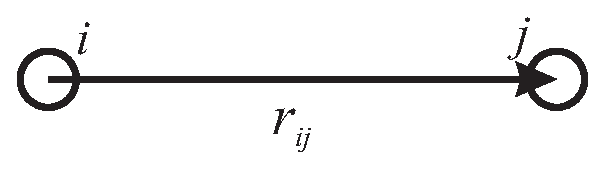
\includegraphics[height=1.6cm]{bond.eps}}
\caption{The interatomic bond vector}
%\vskip 1ex
\end{center}
\end{figure}

The bond potentials describe {\em explicit}
chemical bonds between specified atoms.  They are all
functions of the interatomic distance.  Only the coulomb potential
makes an exception as it depends on the charges of the specified
atoms.  The potential functions available are as follows:
\begin{enumerate}
\item Harmonic bond:  ({\bf harm})
\begin{equation}
U(r_{ij}) = \frac{1}{2} k (r_{ij}-r_{o})^{2}
\end{equation}
\item Morse potential:  ({\bf mors})
\begin{equation}
U(r_{ij}) = E_{o} [\{1-\exp(-k(r_{ij}-r_{o}))\}^{2}-1]
\end{equation}
\item 12-6 potential bond:  ({\bf 12-6})
\begin{equation}
U(r_{ij}) = \left(\frac{A}{r_{ij}^{12}}\right)-\left(\frac{B}{r_{ij}^{6}}\right)
\end{equation}
\item Lennard-Jones potential:  ({\bf lj})
\begin{equation}
U(r_{ij}) = 4\epsilon\left[\left
(\frac{\sigma}{r_{ij}}\right)^{12}-\left(\frac{\sigma}{r_{ij}}\right)^{6}\right]
\end{equation}
\item Restrained harmonic:  ({\bf rhrm})
\begin{equation}
U(r_{ij}) = \left\{ \begin{array} {l@{\quad:\quad}l}
\frac{1}{2}k(r_{ij}-r_{o})^{2} & |r_{ij}-r_{o}|\le r_{c} \\
\frac{1}{2}kr_{c}^{2}+kr_{c}(|r_{ij}-r_{o}|-r_{c}) & |r_{ij}-r_{o}| > r_{c}
\end{array} \right.
\end{equation}
\item Quartic potential:  ({\bf quar})
\begin{equation}
U(r_{ij}) = \frac{k}{2}(r_{ij}-r_{o})^{2}+\frac{k'}{3}(r_{ij}-r_{o})^{3}+\frac{k''}{4}(r_{ij}-r_{o})^{4}
\end{equation}
\item Buckingham potential:  ({\bf buck})
\begin{equation}
U(r_{ij}) = A~\exp\left(-\frac{r_{ij}}{\rho}\right)-\frac{C}{r_{ij}^{6}}
\end{equation}
\item Coulomb potential:  ({\bf coul})
\begin{equation}
U(r_{ij}) = k \cdot U^{Electrostatics}(r_{ij}) \;
\left(= \frac{k}{4\pi\epsilon_{0}\epsilon}\frac{q_{i}q_{j}}{r_{ij}}\right)~~,
\end{equation}
where $q_{\ell}$ is the charge on an atom labelled $\ell$.
It is worth noting that the Coulomb potential switches
to the particular model of Electrostatics opted in CONTROL.
\item Shifted finitely extendible non-linear elastic (FENE) potential \cite{warner-72a,bird-77a,grest-86a}:  ({\bf fene})
\begin{equation}
U(r_{ij}) = \left\{ \begin{array} {l@{\quad:\quad}l}
-0.5~k~R_{o}^{2}~ln\left[1-\left(\frac{r_{ij}-\Delta}{R_{o}}\right)^{2}\right] & |r_{ij} - \Delta| < R_{o} \\
\infty & |r_{ij} - \Delta| \ge R_{o} \end{array} \right. \label{FENE}
\end{equation}
The FENE potential is used to maintain the distance between
connected beads and to prevent chains from crossing each other. It
is used in combination with the WCA, equation~(\ref{wca}), potential to create
a potential well for the flexible bonds of a molecule, that
maintains the topology of the molecule.  This implementation allows
for a radius shift of up to half a $R_{o}$ ($|\Delta| \le
0.5~R_{o}$) with a default of zero ($\Delta_{default} = 0$).
\item MM3 bond stretch potential \cite{allinger-89a}:  ({\bf mmst})
\begin{equation}
U(r_{ij}) = k~(r_{ij}-r_{o})^{2}\left[1-2.55~(r_{ij}-r_{o})+(7/12)~2.55^{2}~(r_{ij}-r_{o})^{2}\right]
\end{equation}
\item Tabulated potential:  ({\bf tab}).  The potential is defined numerically in TABBND (see Section~\ref{bonded-tables} and Section~\ref{intra-tables}).
\end{enumerate}
In these formulae $r_{ij}$ is the distance between atoms labelled
$i$ and $j$:
\begin{equation}
r_{ij} = |\vek{r}_{j}-\vek{r}_{i}|\footnote{{\bf Note}: some \D routines may use the convention
that $\vek{r_{ij}}=\vek{r}_{i}-\vek{r}_{j}$~.}~~,
\end{equation}
where $\vek{r}_{\ell}$ is the position vector of an atom labelled
$\ell$.

The force on the atom $j$ arising from a bond
potential\index{potential!chemical bond} is obtained using the general
formula:
\begin{equation}
\vek{f}_{j} = -\frac{1}{{r}_{ij}} \left[ \frac{\partial }{\partial
r_{ij}}U(r_{ij})\right] \vek{r}_{ij}~~. \label{bondf}
\end{equation}
The force $\vek{f}_{i}$ acting on atom $i$ is the negative of this.

The contribution to be added to the atomic virial is given by
\begin{equation}
{\cal W} = -\vek{r}_{ij} \cdot \vek{f}_{j}~~,
\end{equation}
with only {\em one} such contribution from each bond\index{potential!chemical bond}.

The contribution to be added to the atomic stress
tensor\index{stress tensor} is given by
\begin{equation}
\sigma^{\alpha \beta} = r_{ij}^{\alpha} f_{j}^{\beta}~~, \label{bonds}
\end{equation}
where $\alpha$ and $\beta$ indicate the $x,y,z$ components.  The
atomic stress tensor\index{stress tensor} derived in this way is
symmetric.

In \D bond forces are handled by the routine {\sc bonds\_forces}
(and {\sc intra\_coul} called within).

\subsection{Distance Restraints}

In \D distance restraints, in which the separation between two
atoms, is maintained around some preset value $r_0$ is handled as
a special case of bond potentials.  As a consequence, distance
restraints may be applied only between atoms in the same molecule.
Unlike with application of the ``pure'' bond
potentials\index{potential!chemical bond}, the
electrostatic\index{potential!electrostatics} and van der
Waals\index{potential!van der Waals} interactions between the pair
of atoms are still evaluated when distance restraints are applied.
All the potential forms of the previous section are available as
distance restraints\index{distance restraints}, although they have
different key words:

\begin{enumerate}
\item Harmonic potential:  ({\bf -hrm})
\item Morse potential:  ({\bf -mrs})
\item 12-6 potential bond:  ({\bf -126})
\item Lennard-Jones potential:  ({\bf -lj})
\item Restrained harmonic:  ({\bf -rhm})
\item Quartic potential:  ({\bf -qur})
\item Buckingham potential:  ({\bf -bck})
\item Coulomb potential:  ({\bf -cul})
\item FENE potential:  ({\bf -fne})
\item MM3 bond stretch potential \cite{allinger-89a}:  ({\bf -m3s})
\item Tabulated potential:  ({\bf -tab}).  The potential is defined numerically in TABBND (see Section~\ref{bonded-tables} and Section~\ref{intra-tables}).
\end{enumerate}

In \D distance restraints\index{distance restraints} are handled
by the routine {\sc bonds\_forces} (and {\sc intra\_coul} called within).

\subsection{Valence Angle Potentials}
\label{angle-potentials}

\begin{figure}[htbp]
\begin{center}
\vskip 1ex
\centerline{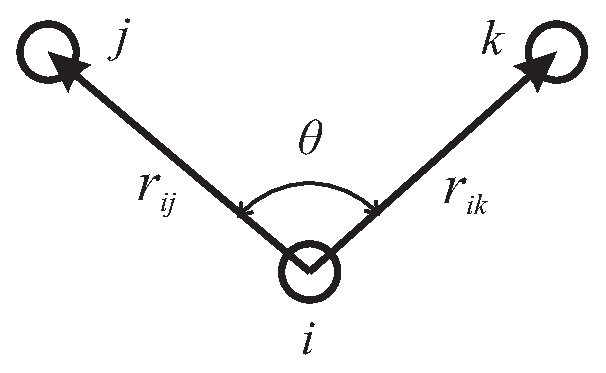
\includegraphics[height=4cm]{angle.eps}}
\caption{The valence angle and associated vectors}
%\vskip 1ex
\end{center}
\end{figure}

The valence angle\index{potential!valence angle} potentials
describe the bond bending terms between the specified atoms.  They
should not be confused with the
three-body\index{potential!three-body} potentials described later,
which are defined by atom types rather than indices.
\begin{enumerate}
\item Harmonic:  ({\bf harm})
\begin{equation}
 U(\theta_{jik}) = {k \over 2} (\theta_{jik} - \theta_0)^{2}
\end{equation}
\item Quartic:  ({\bf quar})
\begin{equation}
 U(\theta_{jik}) = {k \over 2}(\theta_{jik} - \theta_0)^{2} + {k' \over
3}(\theta_{jik} - \theta_0)^{3} + {k'' \over 4}(\theta_{jik} -
\theta_0)^{4}
\end{equation}
\item Truncated harmonic:  ({\bf thrm})
\begin{equation}
U(\theta_{jik}) = {k\over 2} (\theta_{jik} - \theta_0)^{2}
\exp[-(r_{ij}^{8} + r_{ik}^{8}) / \rho^{8}]
\end{equation}
\item Screened harmonic:  ({\bf shrm})
\begin{equation}
 U(\theta_{jik}) = {k\over 2} (\theta_{jik} - \theta_0)^{2}
\exp[-(r_{ij} / \rho_1 + r_{ik} / \rho_2)]
\end{equation}
\item Screened Vessal \cite{vessal-94a}:  ({\bf bvs1})
\begin{eqnarray}
U(\theta_{jik})&=&{k \over 8(\theta_{jik}-\pi)^{2}} \left[ (\theta_0
-\pi)^{2} -(\theta_{jik}-\pi)^{2}\right]^{2} \times \nonumber \\
              & &  \exp[-(r_{ij} / \rho_1 + r_{ik} / \rho_2)]
\end{eqnarray}
\item Truncated Vessal \cite{smith-95a}:  ({\bf bvs2 })
\begin{eqnarray}
U(\theta_{jik})&=& k~(\theta_{jik}-\theta_{0})^{2}~
\big[~\theta_{jik}^a (\theta_{jik}+\theta_{0}-2\pi)^{2} + \nonumber \\
& & {a \over 2} \pi^{a-1} (\theta_{0}-\pi)^{3}~\big]~~\exp[-(r_{ij}^{8} + r_{ik}^{8}) / \rho^{8}]
\end{eqnarray}
\item Harmonic cosine:  ({\bf hcos})
\begin{equation}
U(\theta_{jik}) = {k\over 2}(\cos(\theta_{jik})
-\cos(\theta_{0}))^{2}
\end{equation}
\item Cosine:  ({\bf cos})
\begin{equation}
U(\theta_{jik}) = A~[1 + \cos(m~\theta_{jik}-\delta)]
\end{equation}
\item MM3 stretch-bend \cite{allinger-89a}:  ({\bf mmsb})
\begin{equation}
U(\theta_{jik}) = A~(\theta_{jik}-\theta_{0})~(r_{ij} - r_{ij}^{o})~(r_{ik} - r_{ik}^{o})
\end{equation}
\item Compass stretch-stretch \cite{sun-98a}:  ({\bf stst})
\begin{equation}
U(\theta_{jik}) = A~(r_{ij} - r_{ij}^{o})~(r_{ik} - r_{ik}^{o})
\end{equation}
\item Compass stretch-bend \cite{sun-98a}:  ({\bf stbe})
\begin{equation}
U(\theta_{jik}) = A~(\theta_{jik}-\theta_{0})~(r_{ij} - r_{ij}^{o})
\end{equation}
\item Compass all terms \cite{sun-98a}:  ({\bf cmps})
\begin{equation}
U(\theta_{jik}) = A~(r_{ij} - r_{ij}^{o})~(r_{ik} - r_{ik}^{o}) +
(\theta_{jik}-\theta_{0})~[B~(r_{ij} - r_{ij}^{o})+C~(r_{ik} - r_{ik}^{o})]
\end{equation}
\item MM3 angle bend term \cite{allinger-89a}:  ({\bf m3ab})
\begin{eqnarray}
U(\theta_{jik}) = k~(\theta_{jik}-\theta_{0})^{2}[1 &-& 1.4 \cdot 10^{-2}(\theta_{jik}-\theta_{0})^{~}+5.6 \cdot 10^{-5}(\theta_{jik}-\theta_{0})^{2} \nonumber \\
&-& 7.0 \cdot 10^{-7}(\theta_{jik}-\theta_{0})^{3}+2.2 \cdot 10^{-8}(\theta_{jik}-\theta_{0})^{4}]
\end{eqnarray}
\item KKY \cite{kumagai-94a}:  ({\bf kky})
\begin{eqnarray}
U(\theta_{jik}) &=& f_{k}~\sin\left[2(\theta_{jik}-\theta_{0})\right] \cdot \sqrt{K_{ij} \cdot K_{ik}} \nonumber \\
K_{ij} &=& \frac{1}{\exp\left[g_{r}(r_{ij}-r_{o})\right]}
\end{eqnarray}
\item Tabulated potential:  ({\bf tab}).  The potential is defined numerically in TABANG (see Section~\ref{bonded-tables} and Section~\ref{intra-tables}).
\end{enumerate}
In these formulae $\theta_{jik}$ is the angle between bond vectors
$\vek{r}_{ij}$ and $\vek{r}_{ik}$:
\begin{equation}
\theta_{jik}=cos^{-1}\left\{\frac{\vek{r}_{ij}\cdot\vek{r}_{ik}}
{r_{ij}r_{ik}}\right\}~~.
\end{equation}

In \D the most general form for the valence
angle\index{potential!valence angle}
potentials can be written as:
\begin{equation}
U(\theta_{jik},r_{ij},r_{ik}) = A(\theta_{jik})~S(r_{ij})~S(r_{ik})~S(r_{ik})~~,
\end{equation}
where $A(\theta)$ is a purely angular function and $S(r)$ is a
screening or truncation function.  All the function arguments are
scalars.  With this reduction the force on an atom derived from
the valence angle\index{potential!valence angle} potential is
given by:
\begin{equation}
f_{\ell}^{\alpha} = -\frac{\partial}{\partial
r_{\ell}^{\alpha}}U(\theta_{jik},r_{ij},r_{ik},r_{jk})~~,
\end{equation}
with atomic label $\ell$ being one of $i,j,k$ and $\alpha$
indicating the $x,y,z$ component.  The derivative is
\begin{eqnarray}
-\frac{\partial}{\partial r_{\ell}^{\alpha}}U(\theta_{jik},r_{ij},r_{ik},r_{jk})&=&
-S(r_{ij})S(r_{ik})S(r_{jk})\frac{\partial}{\partial r_{\ell}^{\alpha}}A(\theta_{jik}) \nonumber \\
& & - A(\theta_{jik})S(r_{ik})S(r_{jk})(\delta_{\ell j}-\delta_{\ell i})
\frac{r_{ij}^{\alpha}}{r_{ij}} \frac{\partial}{\partial r_{ij}}S(r_{ij}) \nonumber \\
& & - A(\theta_{jik})S(r_{ij})S(r_{jk})(\delta_{\ell k}-\delta_{\ell i})
\frac{r_{ik}^{\alpha}}{r_{ik}} \frac{\partial}{\partial r_{ik}}S(r_{ik}) \nonumber \\
& & - A(\theta_{jik})S(r_{ij})S(r_{ik})(\delta_{\ell k}-\delta_{\ell j})
\frac{r_{jk}^{\alpha}}{r_{jk}} \frac{\partial}{\partial r_{jk}}S(r_{jk})~~,
\end{eqnarray}
with $\delta_{ab}=1$ if $a=b$ and $\delta_{ab}=0$ if $a\ne b$~.
In the absence of screening terms $S(r)$, this formula reduces to:
\begin{equation}
-\frac{\partial}{\partial
r_{\ell}^{\alpha}}U(\theta_{jik},r_{ij},r_{ik},r_{jk}) =
-\frac{\partial}{\partial r_{\ell}^{\alpha}}A(\theta_{jik})~~.
\end{equation}
The derivative of the angular function is
\begin{equation}
-\frac{\partial}{\partial r_{\ell}^{\alpha}}A(\theta_{jik}) =
\left\{\frac{1}{\sin(\theta_{jik})}\right\}
\frac{\partial}{\partial \theta_{jik}}A(\theta_{jik})
\frac{\partial}{\partial r_{\ell}^{\alpha}}\left\{
\frac{\vek{r}_{ij}\cdot\vek{r}_{ik}}{r_{ij}r_{ik}}\right\}~~,
\end{equation}
with
\begin{eqnarray}
\frac{\partial}{\partial r_{\ell}^{\alpha}}\left\{ \frac{\vek{r}_{ij}\cdot\vek{r}_{ik}}{r_{ij}r_{ik}}\right\}&=&
(\delta_{\ell j}-\delta_{\ell i})\frac{r_{ik}^{\alpha}}{r_{ij}r_{ik}}+ (\delta_{\ell k}-
\delta_{\ell i})\frac{r_{ij}^{\alpha}}{r_{ij}r_{ik}}-\nonumber \\
& & \cos(\theta_{jik}) \left\{(\delta_{\ell j}-\delta_{\ell i})\frac{r_{ij}^{\alpha}}{r_{ij}^{2}}+
(\delta_{\ell k}-\delta_{\ell i})\frac{r_{ik}^{\alpha}}{r_{ik}^{2}}\right\}~~.
\end{eqnarray}
The atomic forces are then completely specified by the derivatives
of the particular functions $A(\theta)$ and $S(r)$~.

The contribution to be added to the atomic virial is given by
\begin{equation}
{\cal W} = -(\vek{r}_{ij} \cdot \vek{f}_{j} + \vek{r}_{ik} \cdot
\vek{f}_{k})~~.
\end{equation}
It is worth noting that in the absence of screening terms S(r), the
virial is zero \cite{smith-93c}.

The contribution to be added to the atomic stress tensor\index{stress tensor} is given by
\begin{equation}
\sigma^{\alpha \beta} = r_{ij}^{\alpha} f_{j}^{\beta} + r_{ik}^{\alpha} f_{k}^{\beta}
\end{equation}
and the stress tensor\index{stress tensor} is symmetric.

In \D valence forces are handled by the routine {\sc
angles\_forces}.

\subsection{Angular Restraints}

In \D angle restraints, in which the angle subtended by a triplet
of atoms, is maintained around some preset value $\theta_{0}$ is
handled as a special case of angle potentials.  As a consequence
angle restraints may be applied only between atoms in the same
molecule.  Unlike with application of the ``pure'' angle
potentials, the electrostatic\index{potential!electrostatics} and
van der Waals\index{potential!van der Waals} interactions between
the pair of atoms are still evaluated when distance restraints are
applied.  All the potential forms of the previous section are
available as angular restraints, although they have different key
words:

\begin{enumerate}
\item Harmonic:  ({\bf -hrm})
\item Quartic:  ({\bf -qur})
\item Truncated harmonic:  ({\bf -thm})
\item Screened harmonic:  ({\bf -shm})
\item Screened Vessal \cite{vessal-94a}:  ({\bf -bv1})
\item Truncated Vessal \cite{smith-95a}:  ({\bf -bv2})
\item Harmonic cosine:  ({\bf -hcs})
\item Cosine:  ({\bf -cos})
\item MM3 stretch-bend \cite{allinger-89a}:  ({\bf -msb})
\item Compass stretch-stretch \cite{sun-98a}:  ({\bf -sts})
\item Compass stretch-bend \cite{sun-98a}:  ({\bf -stb})
\item Compass all terms \cite{sun-98a}:  ({\bf -cmp})
\item MM3 angle bend \cite{allinger-89a}:  ({\bf -m3a})
\item KKY \cite{kumagai-94a}:  ({\bf -kky})
\item Tabulated potential:  ({\bf -tab}).  The potential is defined numerically in TABANG (see Section~\ref{bonded-tables} and Section~\ref{intra-tables}).
\end{enumerate}

In \D angular restraints\index{angular restraints} are handled by
the routine {\sc angles\_forces}.

\subsection{Dihedral Angle Potentials}
\label{dihedral-potentials}

\begin{figure}[htbp]
\begin{center}
\vskip 1ex
\centerline{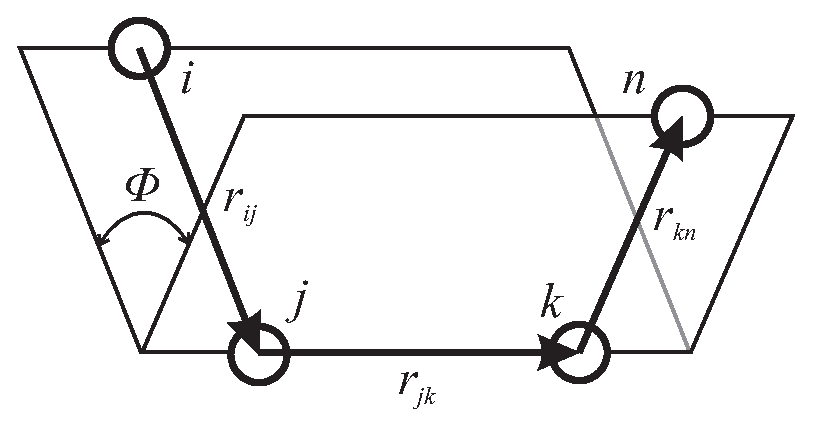
\includegraphics[height=4.9cm]{dihedral.eps}}
\caption{The dihedral angle and associated vectors}
%\vskip 1ex
\end{center}
\end{figure}

The dihedral angle\index{potential!dihedral} potentials describe
the interaction arising from torsional forces in molecules.  (They
are sometimes referred to as torsion potentials.)  They require
the specification of four atomic positions.  The potential
functions available in \D are as follows:
\begin{enumerate}
\item Cosine potential:  ({\bf cos})
\begin{equation}
U(\phi_{ijkn}) = A~\left [ 1 + \cos(m\phi_{ijkn} - \delta)\right]
\end{equation}
\item Harmonic:  ({\bf harm})
\begin{equation}
U(\phi_{ijkn}) = {k \over 2}~(\phi_{ijkn} - \phi_{0})^{2}
\end{equation}
\item Harmonic cosine:  ({\bf hcos})
\begin{equation}
U(\phi_{ijkn}) = {k \over 2}~(\cos(\phi_{ijkn}) - \cos(\phi_{0}))^{2}
\end{equation}
\item Triple cosine:  ({\bf cos3})
\begin{equation}
U(\phi) = {1 \over 2}~\{A_{1}~(1+\cos(\phi)) + A_{2}~(1-\cos(2\phi)) + A_{3}~(1+\cos(3\phi))\}
\end{equation}
\item Ryckaert-Bellemans \cite{ryckaert-75a} with fixed constants
a-f: ({\bf ryck})
\begin{equation}
U(\phi) = A~\{~a+b~\cos(\phi)+c~\cos^{2}(\phi)+d~\cos^{3}(\phi)+e~\cos^{4}(\phi)+f~\cos^{5}(\phi)~\}
\end{equation}
\item Fluorinated Ryckaert-Bellemans \cite{schmidt-96a} with fixed
constants a-h:  ({\bf rbf})
\begin{eqnarray}
U(\phi) = A~\{~a+b~\cos(\phi)+c~\cos^{2}(\phi)+d~\cos^{3}(\phi)+e~\cos^{4}(\phi)+f~\cos^{5}(\phi)+ \nonumber \\
~g~\exp(-h(\phi-\pi)^{2}))~\}
\end{eqnarray}
\item OPLS torsion potential:  ({\bf opls})
\begin{equation}
U(\phi)=A_{0}+\frac{1}{2} \left\{ A_{1}~(1+\cos(\phi))+A_{2}~(1-\cos(2\phi))+A_{3}~(1+\cos(3\phi)) \right\}
\end{equation}
\item Tabulated potential:  ({\bf tab}).  The potential is defined numerically in TABDIH (see Section~\ref{bonded-tables} and Section~\ref{intra-tables}).
\end{enumerate}
In these formulae $\phi_{ijkn}$ is the dihedral angle defined by
\begin{equation}
\phi_{ijkn}=\cos^{-1}\{B(\vek{r}_{ij},\vek{r}_{jk},\vek{r}_{kn})\}~~,
\end{equation}
with
\begin{equation}
B(\vek{r}_{ij},\vek{r}_{jk},\vek{r}_{kn})= \left\{\frac{
(\vek{r}_{ij}\times\vek{r}_{jk})\cdot(\vek{r}_{jk}\times\vek{r}_{kn})}
{|\vek{r}_{ij}\times\vek{r}_{jk}||\vek{r}_{jk}\times\vek{r}_{kn}|}
\right\}~~.
\end{equation}
With this definition, the sign of the
dihedral\index{potential!dihedral} angle is positive if the vector
product \linebreak[4] \mbox{$(\vek{r}_{ij} \times \vek{r}_{jk})
\times (\vek{r}_{jk} \times \vek{r}_{kn})$} is in the same
direction as the bond\index{potential!chemical bond} vector $\vek{r}_{jk}$
and negative if in the opposite direction.

The force on an atom arising from the dihedral\index{potential!dihedral} potential is given by
\begin{equation}
f_{\ell}^{\alpha}=-\frac{\partial}{\partial
r_{\ell}^{\alpha}}U(\phi_{ijkn})~~,
\end{equation}
with $\ell$ being one of $i,j,k,n$ and $\alpha$ one of $x,y,z$.
This may be expanded into
\begin{equation}
-\frac{\partial}{\partial r_{\ell}^{\alpha}}U(\phi_{ijkn})=
\left\{\frac{1}{\sin(\phi_{ijkn})}\right\}
\frac{\partial}{\partial \phi_{ijkn}}U(\phi_{ijkn})
\frac{\partial}{\partial r_{\ell}^{\alpha}}
B(\vek{r}_{ij},\vek{r}_{jk},\vek{r}_{kn})~~.
\end{equation}
The derivative of the function
$B(\vek{r}_{ij},\vek{r}_{jk},\vek{r}_{kn})$ is
\begin{eqnarray}
& &\frac{\partial}{\partial r_{\ell}^{\alpha}}
B(\vek{r}_{ij},\vek{r}_{jk},\vek{r}_{kn})~=~
\frac{1}{|\vek{r}_{ij}\times\vek{r}_{jk}||\vek{r}_{jk}\times\vek{r}_{kn}|}
\frac{\partial}{\partial r_{\ell}^{\alpha}}
\{(\vek{r}_{ij}\times\vek{r}_{jk})\cdot(\vek{r}_{jk}\times\vek{r}_{kn})\}~-~~~~\nonumber \\
& & \phantom{x} \frac{\cos(\phi_{ijkn})}{2}\left\{
\frac{1}{|\vek{r}_{ij}\times\vek{r}_{jk}|^{2}}
\frac{\partial}{\partial r_{\ell}^{\alpha}}
|\vek{r}_{ij}\times\vek{r}_{jk}|^{2}+
\frac{1}{|\vek{r}_{jk}\times\vek{r}_{kn}|^{2}}
\frac{\partial}{\partial r_{\ell}^{\alpha}}
|\vek{r}_{jk}\times\vek{r}_{kn}|^{2} \right\}~~,
\end{eqnarray}
with
\begin{eqnarray}
\frac{\partial}{\partial r_{\ell}^{\alpha}}
\{(\vek{r}_{ij}\times\vek{r}_{jk})\cdot(\vek{r}_{jk}\times\vek{r}_{kn})\}&=&
r_{ij}^{\alpha}([\vek{r}_{jk}\vek{r}_{jk}]_{\alpha}(\delta_{\ell k}-\delta_{\ell n})+
 [\vek{r}_{jk}\vek{r}_{kn}]_{\alpha}(\delta_{\ell k}-\delta_{\ell j}))+ \nonumber \\
\phantom{\frac{\partial}{\partial r_{\ell}^{\alpha}}}& &
r_{jk}^{\alpha}([\vek{r}_{ij}\vek{r}_{jk}]_{\alpha}
(\delta_{\ell n}-\delta_{\ell k})+ [\vek{r}_{jk}\vek{r}_{kn}]_{\alpha}
(\delta_{\ell j}-\delta_{\ell i}))+ \nonumber \\
\phantom{\frac{\partial}{\partial r_{\ell}^{\alpha}}} & &
r_{kn}^{\alpha}([\vek{r}_{ij}\vek{r}_{jk}]_{\alpha}(\delta_{\ell k}-\delta_{\ell j})+
[\vek{r}_{jk}\vek{r}_{jk}]_{\alpha}(\delta_{\ell i}-\delta_{\ell j}))+ \nonumber \\
\phantom{\frac{\partial}{\partial r_{\ell}^{\alpha}}} & &
2r_{jk}^{\alpha}[\vek{r}_{ij}\vek{r}_{kn}]_{\alpha}(\delta_{\ell j}-\delta_{\ell k})~~,
\end{eqnarray}
\begin{eqnarray}
\frac{\partial}{\partial r_{\ell}^{\alpha}}
|\vek{r}_{ij}\times\vek{r}_{jk}|^{2}&=&
2r_{ij}^{\alpha}([\vek{r}_{jk}\vek{r}_{jk}]_{\alpha}(\delta_{\ell j}-\delta_{\ell i})+
[\vek{r}_{ij}\vek{r}_{jk}]_{\alpha}(\delta_{\ell j}-\delta_{\ell k}))+\nonumber \\
& & 2r_{jk}^{\alpha}([\vek{r}_{ij}\vek{r}_{ij}]_{\alpha}
(\delta_{\ell k}-\delta_{\ell j}) +[\vek{r}_{ij}\vek{r}_{jk}]_{\alpha}
(\delta_{\ell i}-\delta_{\ell j}))~~,
\end{eqnarray}
\begin{eqnarray}
\frac{\partial}{\partial r_{\ell}^{\alpha}}
|\vek{r}_{jk}\times\vek{r}_{kn}|^{2}&=&
2r_{kn}^{\alpha}([\vek{r}_{jk}\vek{r}_{jk}]_{\alpha}(\delta_{\ell n}-\delta_{\ell k})+
[\vek{r}_{jk}\vek{r}_{kn}]_{\alpha}(\delta_{\ell j}-\delta_{\ell k}))+\nonumber \\
& & 2r_{jk}^{\alpha}([\vek{r}_{kn}\vek{r}_{kn}]_{\alpha}
(\delta_{\ell k}-\delta_{\ell j})+
[\vek{r}_{jk}\vek{r}_{kn}]_{\alpha}(\delta_{\ell k}-\delta_{\ell n}))~~.
\end{eqnarray}
Where we have used the following definition:
\begin{equation}
[\vek{a}~\vek{b}]_{\alpha} =
\sum_{\beta}(1-\delta_{\alpha\beta})a^{\beta}b^{\beta}~~.
\end{equation}

Formally, the contribution to be added to the atomic virial is given
by
\begin{equation}
{\cal W}=-\sum_{i=1}^{4} \vek{r}_{i} \cdot \vek{f}_{i}~~.
\end{equation}

However, it is possible to show (by tedious algebra using the
above formulae, or more elegantly by thermodynamic arguments
\cite{smith-93c},) that the dihedral makes {\em no} contribution
to the atomic virial.

The contribution to be added to the atomic stress tensor\index{stress tensor} is given by
\begin{eqnarray}
\sigma^{\alpha \beta}&=&r_{ij}^{\alpha}p_{i}^{\beta}+
r_{jk}^{\alpha}p_{jk}^{\beta}+r_{kn}^{\alpha}p_{n}^{\beta} \\ & &
-\frac{\cos(\phi_{ijkn})}{2}\left \{r_{ij}^{\alpha}g_{i}^{\beta}+
r_{jk}^{\alpha}g_{k}^{\beta}+r_{jk}^{\alpha}h_{j}^{\beta}+r_{kn}^{\alpha}h_{n}^{\beta}\right\}
~~,\nonumber
\end{eqnarray}
with
\begin{eqnarray}
p_{i}^{\alpha}&=&(r_{jk}^{\alpha}[\vek{r}_{jk}\vek{r}_{kn}]_{\alpha}-
r_{kn}^{\alpha}[\vek{r}_{jk}\vek{r}_{jk}]_{\alpha})/
(|\vek{r}_{ij}\times\vek{r}_{jk}||\vek{r}_{jk}\times\vek{r}_{kn}|) \nonumber \\
p_{n}^{\alpha}&=&(r_{jk}^{\alpha}[\vek{r}_{ij}\vek{r}_{jk}]_{\alpha}-
r_{ij}^{\alpha}[\vek{r}_{jk}\vek{r}_{jk}]_{\alpha})/
(|\vek{r}_{ij}\times\vek{r}_{jk}||\vek{r}_{jk}\times\vek{r}_{kn}|) \nonumber \\
p_{jk}^{\alpha}&=&(r_{ij}^{\alpha}[\vek{r}_{jk}\vek{r}_{kn}]_{\alpha}+
r_{kn}^{\alpha}[\vek{r}_{ij}\vek{r}_{jk}]_{\alpha}-
2r_{jk}^{\alpha}[\vek{r}_{ij}\vek{r}_{kn}]_{\alpha})/
(|\vek{r}_{ij}\times\vek{r}_{jk}||\vek{r}_{jk}\times\vek{r}_{kn}|) \nonumber \\
g_{i}^{\alpha}&=&2(r_{ij}^{\alpha}[\vek{r}_{jk}\vek{r}_{jk}]_{\alpha}-
r_{jk}^{\alpha}[\vek{r}_{ij}\vek{r}_{jk}]_{\alpha})/
|\vek{r}_{ij}\times\vek{r}_{jk}|^{2} \\
g_{k}^{\alpha}&=&2(r_{jk}^{\alpha}[\vek{r}_{ij}\vek{r}_{ij}]_{\alpha}-
r_{ij}^{\alpha}[\vek{r}_{ij}\vek{r}_{jk}]_{\alpha})/
|\vek{r}_{ij}\times\vek{r}_{jk}|^{2} \nonumber \\
h_{j}^{\alpha}&=&2(r_{jk}^{\alpha}[\vek{r}_{kn}\vek{r}_{kn}]_{\alpha}-
r_{kn}^{\alpha}[\vek{r}_{jk}\vek{r}_{kn}]_{\alpha})/
|\vek{r}_{jk}\times\vek{r}_{kn}|^{2} \nonumber \\
h_{n}^{\alpha}&=&2(r_{kn}^{\alpha}[\vek{r}_{kn}\vek{r}_{kn}]_{\alpha}-
r_{jk}^{\alpha}[\vek{r}_{jk}\vek{r}_{kn}]_{\alpha})/
|\vek{r}_{jk}\times\vek{r}_{kn}|^{2}~~. \nonumber
\end{eqnarray}
The sum of the diagonal elements of the stress tensor\index{stress
tensor} is zero (since the virial is zero) and the matrix is
symmetric.

Lastly, it should be noted that the above description does not
take into account the possible inclusion of distance-dependent 1-4
interactions, as permitted by some force fields\index{force
field}.  Such interactions are permissible in \D and are described
in the section on pair potentials below.  \D also permits scaling
of the 1-4 van der Waals\index{potential!van der Waals} and Coulomb
\index{potential!electrostatics} interactions by a numerical
factor (see Table~\ref{dihedral-table}).  {\bf Note} that scaling
is abandoned when the 1-4 members are also 1-3 members in a valence
angle\index{potential!valence angle} intercation (1-4 checks are
performed in {\sc dihedrals\_14\_check} routine).  1-4 interactions
do, of course, contribute to the atomic virial.

In \D dihedral forces are handled by the routine {\sc dihedrals\_forces}
(and {\sc intra\_coul} and {\sc dihedrals\_14\_vdw} called within).

\subsection{Improper Dihedral Angle Potentials}
\label{improper-dihedral-potentials}

Improper dihedrals\index{potential!improper dihedral} are used to
restrict the geometry of molecules and as such need not have a
simple relation to conventional chemical
bonding\index{potential!chemical bond}.  \D makes no distinction between
dihedral\index{potential!dihedral} and improper
dihedral\index{potential!improper dihedral} angle functions (both
are calculated by the same subroutines) and all the comments made
in the preceding section apply.

An important example of the use of the improper
dihedral\index{potential!improper dihedral} is to conserve the
structure of chiral centres in molecules modelled by united-atom
centres. For example $\alpha$-amino acids such as alanine
(CH$_{3}$CH(NH$_{2}$)COOH), in which it is common to represent the
CH$_{3}$ and CH groups as single centres.  Conservation of the
chirality of the $\alpha$ carbon is achieved by defining a
harmonic improper dihedral angle\index{potential!dihedral}
potential with an equilibrium angle of 35.264$^{o}$.  The angle is
defined by vectors $\vek{r}_{12}$, $\vek{r}_{23}$ and
$\vek{r}_{34}$, where the atoms 1,2,3 and 4 are shown in the
following figure.  The figure defines the D and L enantiomers
consistent with the international (IUPAC) convention.  When
defining the dihedral\index{potential!dihedral}, the atom indices
are entered in \D in the order 1-2-3-4.

\begin{figure}[htbp]
\begin{center}
\vskip 1ex
\centerline{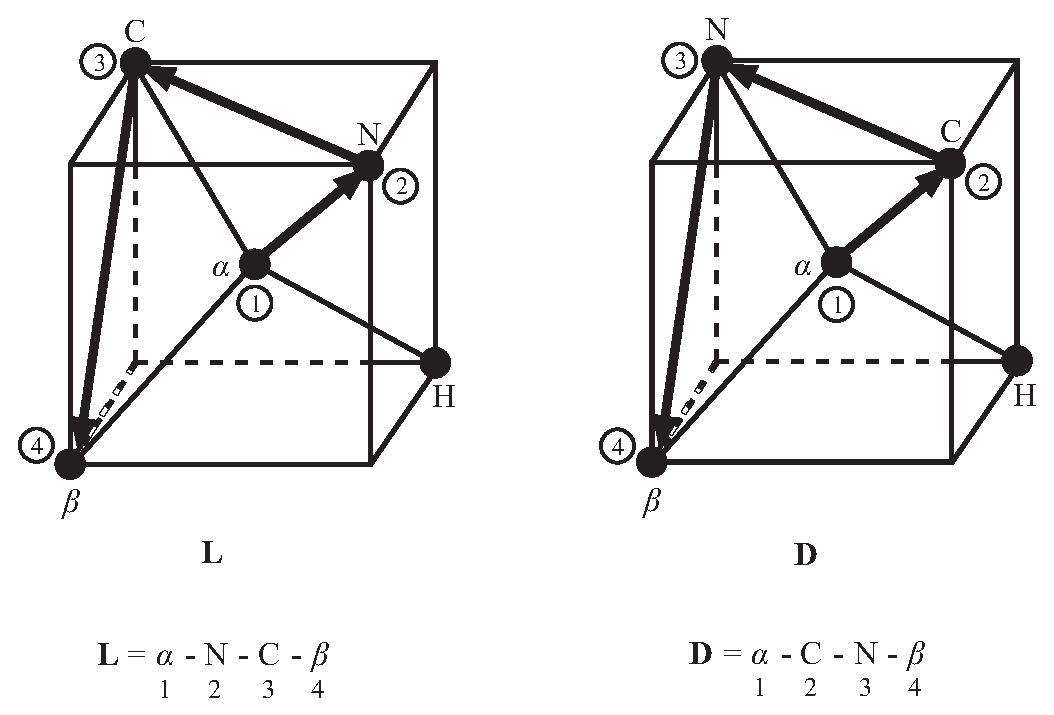
\includegraphics[height=9.5cm]{isomers.eps}}
\caption{The L and D enantiomers and defining vectors}
%\vskip 1ex
\end{center}
\end{figure}

In \D improper dihedral forces\index{potential!improper dihedral}
are handled by the routine {\sc dihedrals\_forces}.

\subsection{Torsional Restraints}

In \D the torsional restraints, in which the dihedral angle as defined
by a quadruplet of atoms, is maintained around some preset value $\phi_{0}$
is handled as a special case of dihedral potential.
As a consequence angle restraints may be applied only between atoms
in the same molecule.  Unlike with application of the ``pure'' dihedral
potentials, the electrostatic\index{potential!electrostatics} and
van der Waals\index{potential!van der Waals} interactions between
the pair of atoms are still evaluated when distance restraints are
applied.  All the potential forms of the previous section are
available as torsional restraints, although they have different key
words:

\begin{enumerate}
\item Cosine potential:  ({\bf -cos})
\item Harmonic:  ({\bf -hrm})
\item Harmonic cosine:  ({\bf -hcs})
\item Triple cosine:  ({\bf -cs3})
\item Ryckaert-Bellemans \cite{ryckaert-75a} with fixed constants
a-f: ({\bf -rck})
\item Fluorinated Ryckaert-Bellemans \cite{schmidt-96a} with fixed
constants a-h:  ({\bf -rbf})
\item OPLS torsion potential:  ({\bf -opl})
\item Tabulated potential:  ({\bf -tab}).  The potential is defined numerically in TABDIH (see Section~\ref{bonded-tables} and Section~\ref{intra-tables}).
\end{enumerate}

In \D torsional restraints\index{torsional restraints} are handled by
the routine {\sc dihedrals\_forces}.

\subsection{Inversion Angle Potentials}
\label{inversion-potentials}

\begin{figure}[htbp]
\begin{center}
\vskip 1ex
\centerline{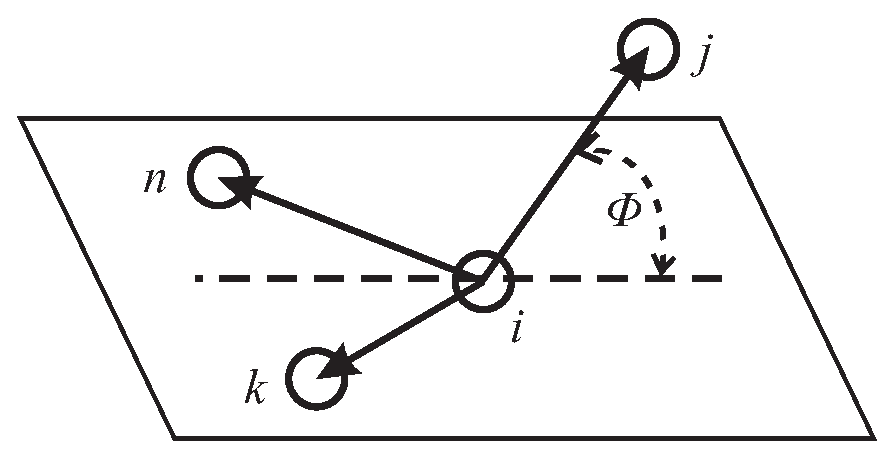
\includegraphics[height=4.9cm]{inversion.eps}}
\caption{The inversion angle and associated vectors}
%\vskip 1ex
\end{center}
\end{figure}

The inversion angle potentials\index{potential!inversion} describe
the interaction arising from a particular geometry of three atoms
around a central atom.  The best known example of this is the
arrangement of hydrogen atoms around nitrogen in ammonia to form a
trigonal pyramid.  The hydrogens can `flip' like an inverting
umbrella to an alternative structure, which in this case is
identical, but in principle causes a change in chirality.  The
force restraining the ammonia to one structure can be described as
an inversion potential\index{potential!inversion} (though it is
usually augmented by valence\index{potential!valence angle} angle
potentials also).  The inversion angle is defined in the figure
above - {\bf note that the inversion\index{potential!inversion}
angle potential is a sum of the three possible
inversion\index{potential!inversion} angle terms}.  It resembles a
dihedral\index{potential!dihedral} potential in that it requires
the specification of four atomic positions.

The potential functions available in \D are as follows:
\begin{enumerate}
\item Harmonic:  ({\bf harm})
\begin{equation}
U(\phi_{ijkn}) = {k \over 2}~(\phi_{ijkn} - \phi_{0})^{2}
\end{equation}
\item Harmonic cosine:  ({\bf hcos})
\begin{equation}
U(\phi_{ijkn}) = {k \over 2}~(\cos(\phi_{ijkn}) - \cos(\phi_{0}))^{2}
\end{equation}
\item Planar potential:  ({\bf plan})
\begin{equation}
U(\phi_{ijkn}) = A~\left[ 1 - \cos(\phi_{ijkn}) \right]
\end{equation}
\item Extended planar potential:  ({\bf xpln})
\begin{equation}
U(\phi_{ijkn}) = {k \over 2}~\left[ 1 - \cos(m~\phi_{ijkn} - \phi_{0}) \right]
\end{equation}
\item Tabulated potential:  ({\bf tab}).  The potential is defined numerically in TABINV (see Section~\ref{bonded-tables} and Section~\ref{intra-tables}).
\end{enumerate}
In these formulae $\phi_{ijkn}$ is the
inversion\index{potential!inversion} angle defined by
\begin{equation}
\phi_{ijkn}=\cos^{-1} \left\{ \frac{\vek{r}_{ij}\cdot\vek{w}_{kn}}{r_{ij}w_{kn}} \right\}~~,
\end{equation}
with
\begin{equation}
\vek{w}_{kn}=(\vek{r}_{ij}\cdot\vek{\hat{u}}_{kn})\vek{\hat{u}}_{kn}+
(\vek{r}_{ij}\cdot\vek{\hat{v}}_{kn})\vek{\hat{v}}_{kn}
\end{equation}
and the unit vectors
\begin{eqnarray}
\vek{\hat{u}}_{kn}&=&(\vek{\hat{r}}_{ik}+\vek{\hat{r}}_{in})/
|\vek{\hat{r}}_{ik}+\vek{\hat{r}}_{in}| \nonumber  \\
\vek{\hat{v}}_{kn}&=&(\vek{\hat{r}}_{ik}-\vek{\hat{r}}_{in})/
|\vek{\hat{r}}_{ik}-\vek{\hat{r}}_{in}|~~.
\end{eqnarray}
As usual, $\vek{r}_{ij}=\vek{r}_{j}-\vek{r}_{i}$ {\em etc.} and
the hat $\vek{\hat{r}}$ indicates a {\em unit} vector in the
direction of $\vek{r}$.  The total
inversion\index{potential!inversion} potential requires the
calculation of three such angles, the formula being derived from
the above using the cyclic permutation of the indices $j
\rightarrow k \rightarrow n \rightarrow j$ {\em etc}.

Equivalently, the angle $\phi_{ijkn}$ may be written as
\begin{equation}
\phi_{ijkn} = \cos^{-1} \left\{ \frac{ [
(\vek{r}_{ij}\cdot\vek{\hat{u}}_{kn})^{2} +
(\vek{r}_{ij}\cdot\vek{\hat{v}}_{kn})^{2}
]^{1/2}}{r_{ij}} \right\}~~.
\end{equation}

Formally, the force on an atom arising from the
inversion\index{potential!inversion} potential is given by
\begin{equation}
f_{\ell}^{\alpha} = -\frac{\partial}{\partial
r_{\ell}^{\alpha}}U(\phi_{ijkn})~~,
\end{equation}
with $\ell$ being one of $i,j,k,n$ and $\alpha$ one of $x,y,z$.
This may be expanded into
\begin{eqnarray}
-\frac{\partial}{\partial r_{\ell}^{\alpha}}U(\phi_{ijkn})&=&
\left\{ \frac{1}{\sin(\phi_{ijkn})} \right\}
\frac{\partial}{\partial \phi_{ijkn}}U(\phi_{ijkn})\times \nonumber \\
& & \frac{\partial}{\partial r_{\ell}^{\alpha}} \left\{
\frac{[(\vek{r}_{ij}\cdot\vek{\hat{u}}_{kn})^{2}
+(\vek{r}_{ij}\cdot\vek{\hat{v}}_{kn})^{2}]^{1/2}} {r_{ij}}
\right\}~~.
\end{eqnarray}
Following through, the (extremely tedious!) differentiation gives
the result:
\begin{eqnarray}
f_{\ell}^{\alpha} &=&
\left\{\frac{1}{\sin(\phi_{ijkn})}\right\}
\frac{\partial}{\partial \phi_{ijkn}}U(\phi_{ijkn})\times \\
& &
\left\{-(\delta_{\ell j}-\delta_{\ell i})\frac{\cos(\phi_{ijkn})}
{r_{ij}^{2}}r_{ij}^{\alpha} +\frac{1}{r_{ij}w_{kn}}\left [
(\delta_{\ell j}-\delta_{\ell i})
\{(\vek{r}_{ij}\cdot\vek{\hat{u}}_{kn})\hat{u}_{kn}^{\alpha}+
(\vek{r}_{ij}\cdot\vek{\hat{v}}_{kn})\hat{v}_{kn}^{\alpha}\}
\phantom{\left\{\frac{a_{a}^{a}}{a_{a}^{a}}\right\}}
\right. \right. \nonumber \\
& & + (\delta_{\ell k}-\delta_{\ell i})
\frac{\vek{r}_{ij}\cdot\vek{\hat{u}}_{kn}}{u_{kn}r_{ik}}\left \{
r_{ij}^{\alpha}-(\vek{r}_{ij}\cdot\vek{\hat{u}}_{kn})\hat{u}_{kn}^{\alpha}
-(\vek{r}_{ij}\cdot\vek{r}_{ik}-(\vek{r}_{ij}\cdot\vek{\hat{u}}_{kn})
(\vek{r}_{ik}\cdot\vek{\hat{u}}_{kn}))\frac{r_{ik}^{\alpha}}{r_{ik}^{2}}
\right \} \nonumber \\
& & + (\delta_{\ell k}-\delta_{\ell i})
\frac{\vek{r}_{ij}\cdot\vek{\hat{v}}_{kn}}{v_{kn}r_{ik}}\left \{
r_{ij}^{\alpha}-(\vek{r}_{ij}\cdot\vek{\hat{v}}_{kn})\hat{v}_{kn}^{\alpha}
-(\vek{r}_{ij}\cdot\vek{r}_{ik}-(\vek{r}_{ij}\cdot\vek{\hat{v}}_{kn})
(\vek{r}_{ik}\cdot\vek{\hat{v}}_{kn}))\frac{r_{ik}^{\alpha}}{r_{ik}^{2}}
\right \} \nonumber \\
& &+ (\delta_{\ell n}-\delta_{\ell i})
\frac{\vek{r}_{ij}\cdot\vek{\hat{u}}_{kn}}{u_{kn}r_{in}}\left \{
r_{ij}^{\alpha}-(\vek{r}_{ij}\cdot\vek{\hat{u}}_{kn})\hat{u}_{kn}^{\alpha}
-(\vek{r}_{ij}\cdot\vek{r}_{in}-(\vek{r}_{ij}\cdot\vek{\hat{u}}_{kn})
(\vek{r}_{in}\cdot\vek{\hat{u}}_{kn}))\frac{r_{in}^{\alpha}}{r_{in}^{2}}
\right \} \nonumber \\
& & \left . \left .- (\delta_{\ell n}-\delta_{\ell i})
\frac{\vek{r}_{ij}\cdot\vek{\hat{v}}_{kn}}{v_{kn}r_{in}}\left \{
r_{ij}^{\alpha}-(\vek{r}_{ij}\cdot\vek{\hat{v}}_{kn})\hat{v}_{kn}^{\alpha}
-(\vek{r}_{ij}\cdot\vek{r}_{in}-(\vek{r}_{ij}\cdot\vek{\hat{v}}_{kn})
(\vek{r}_{in}\cdot\vek{\hat{v}}_{kn}))\frac{r_{in}^{\alpha}}{r_{in}^{2}}
\right \} \right ] \right \}~~. \nonumber
\end{eqnarray}
This general formula applies to all atoms $\ell=i,j,k,n$.  It must
be remembered however, that these formulae apply to just one of
the three contributing terms (i.e. one angle $\phi$) of the full
inversion\index{potential!inversion} potential: specifically the
inversion\index{potential!inversion} angle pertaining to the
out-of-plane vector $\vek{r}_{ij}$~.  The contributions arising
from the other vectors $\vek{r}_{ik}$ and $\vek{r}_{in}$ are
obtained by the cyclic permutation of the indices in the manner
described above.  All these force contributions must be added to
the final atomic forces.

Formally, the contribution to be added to the
atomic virial is given by
\begin{equation}
{\cal W} = -\sum_{i=1}^{4}\vek{r}_{i} \cdot \vek{f}_{i}~~.
\end{equation}
However, it is possible to show by thermodynamic arguments ({\em
cf} \cite{smith-93c},) or simply from the fact that the sum of
forces on atoms j,k and n is equal and opposite to the force on
atom i, that the inversion potential
makes\index{potential!inversion} {\em no} contribution to the
atomic virial.

If the force components $f_{\ell}^{\alpha}$ for atoms $\ell=i,j,k,n$ are
calculated using the above formulae, it is easily seen that
the contribution to be added to the atomic stress tensor\index{stress tensor} is given by
\begin{equation}
\sigma^{\alpha \beta} = r_{ij}^{\alpha} f_{j}^{\beta} +
r_{ik}^{\alpha} f_{k}^{\beta}+r_{in}^{\alpha}f_{n}^{\beta}~~.
\end{equation}
The sum of the diagonal elements of the stress tensor\index{stress tensor} is zero (since
the virial is zero) and the matrix is symmetric.

In \D inversion\index{potential!inversion} forces are handled by
the routine {\sc inversions\_forces}.

\subsection{The Calcite Four-Body Potential}
\label{calcite}

\begin{figure}[htbp]
\begin{center}
\vskip 1ex
\centerline{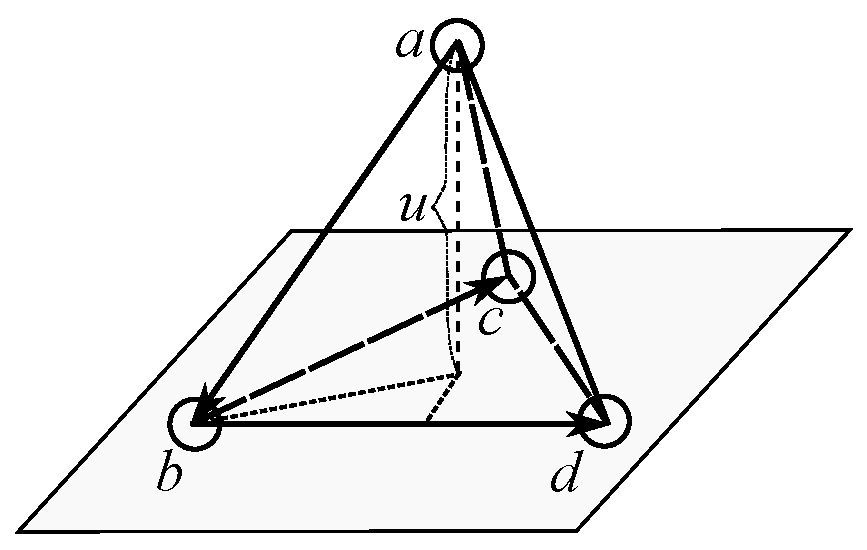
\includegraphics[height=6.9cm]{calcite.eps}}
\caption{The vectors of the calcite potential}
\label{calcfig}
%\vskip 1ex
\end{center}
\end{figure}

\index{potential!calcite} This potential \cite{rohl-03a,raiteri-10a} is designed to
help maintain the planar structure of the carbonate anion $[CO_{3}]^{2-}$ in a
similar manner to the planar inversion potential described above.  However,
it is {\em not} an angular potential.  It is dependent on the perpendicular
displacement ($u$) of an atom $a$ from a plane defined by three other atoms
$b$, $c$, and $d$ (see Figure~\ref{calcfig}) and has the form:
\begin{equation}
U_{abcd}(u)=Au^{2}+Bu^{4}~~, \label{calcite1}
\end{equation}
where the displacement $u$ is given by
\begin{equation}
u=\frac{\vek{r}_{ab}\cdot\vek{r}_{bc}\times\vek{r}_{bd}}{|\vek{r}_{bc}\times\vek{r}_{bd}|}~~. \label{calcite2}
\end{equation}
Vectors $\vek{r}_{ab}$,$\vek{r}_{ac}$ and $\vek{r}_{ad}$ define bonds between
the central atom $a$ and the peripheral atoms $b$, $c$ and $d$.  Vectors
$\vek{r}_{bc}$ and $\vek{r}_{bd}$ define the plane and are related to the bond
vectors by
\begin{eqnarray}
\vek{r}_{bc}&=&\vek{r}_{ac}-\vek{r}_{ab} \nonumber \\
\vek{r}_{bd}&=&\vek{r}_{ad}-\vek{r}_{ab}~~.
\end{eqnarray}
In what follows it is convenient to define the vector product appearing in
both the numerator and denominator of equation~(\ref{calcite2}) as the vector
$\vek{w}_{cd}$ {\em vis.}
\begin{equation}
\vek{w}_{cd}=\vek{r}_{bc}\times\vek{r}_{bd}~~.
\end{equation}
We also define the quantity $\gamma(u)$ as
\begin{equation}
\gamma(u)=-(2Au+4Bu^{3})~~.
\end{equation}
The forces on the individual atoms due to the calcite potential are
then given by
\begin{eqnarray}
\vek{f}_{a}&=&-\gamma(u)~\hat{\vek{w}}_{cd} \nonumber \\
\vek{f}_{c}&=&\phantom{+}\vek{r}_{bd}\times(\vek{r}_{ab}-u\hat{\vek{w}}_{cd})~\gamma(u)/w_{cd} \nonumber \\
\vek{f}_{d}&=&-\vek{r}_{bc}\times(\vek{r}_{ab}- u\hat{\vek{w}}_{cd})~\gamma(u)/w_{cd} \\
\vek{f}_{b}&=&-(\vek{f}_{a}+\vek{f}_{c}+\vek{f}_{d})~~,\nonumber
\end{eqnarray}
where $w_{cd}=|\vek{w}_{cd}|$ and $\hat{\vek{w}}_{cd}=\vek{w}_{cd}/w_{cd}$.
The virial contribution $\psi_{abcd}(u)$ is given by
\begin{equation}
\psi_{abcd}(u)=2Au^{2}+4Bu^{4}
\end{equation}
and the stress tensor contribution $\sigma_{abcd}^{\alpha\beta}(u)$ by
\begin{equation}
\sigma_{abcd}^{\alpha\beta}(u)=\frac{u~\gamma(u)}{w_{cd}^{2}}~w_{cd}^{\alpha}~w_{cd}^{\beta}~~.
\end{equation}

In \D the calcite\index{potential!calcite} forces are handled by the routine
{\sc inversions\_forces}, which is a convenient {\em intramolecular} four-body
force routine. However, it is manifestly {\em not} an inversion potential as such.

\subsection{Inversional Restraints}

In \D the inversional restraints, in which the inversion angle, as defined
by a quadruplet of atoms, is maintained around some preset value $\phi_{0}$,
is handled as a special case of  inversion potential.
As a consequence angle restraints may be applied only between atoms
in the same molecule.  Unlike with application of the ``pure'' dihedral
potentials, the electrostatic\index{potential!electrostatics} and
van der Waals\index{potential!van der Waals} interactions between
the pair of atoms are still evaluated when distance restraints are
applied.  All the potential forms of the previous section are
available as torsional restraints, although they have different key
words:

\begin{enumerate}
\item Harmonic:  ({\bf -hrm})
\item Harmonic cosine:  ({\bf -hcs})
\item Planar potential:  ({\bf -pln})
\item Extended planar potential:  ({\bf -xpl})
\item Tabulated potential:  ({\bf -tab}).  The potential is defined numerically in TABINV (see Section~\ref{bonded-tables} and Section~\ref{intra-tables}).
\end{enumerate}

In \D inversional restraints\index{inversional restraints} are handled by
the routine {\sc inversions\_forces}.

\subsection{Tethering Forces}

\D also allows atomic sites to be tethered\index{potential!tether}
to a fixed point in space, $\vec{r_{0}}$, taken as their position
at the beginning of the simulation (t~=~0).  This is also known as
position restraining.  The specification, which comes as part of
the molecular description, requires a tether potential type and
the associated interaction parameters.

{\bf Note}, firstly, that application of tethering potentials means that
the momentum will no longer be a conserved quantity of the
simulation.  Secondly, in constant pressure simulations, where the
MD cell changes size or shape, the tethers' reference positions
are scaled with the cell vectors.

The tethering potential functions available in \D are as follows:
\begin{enumerate}
\item Harmonic:  ({\bf harm})
\begin{equation}
U(r_{ij}) = \frac{1}{2}k(r_{i0})^{2}
\end{equation}
\item Restrained harmonic:  ({\bf rhrm})
\begin{equation}
U(r_{ij}) = \left\{ \begin{array} {l@{\quad:\quad}l}
\frac{1}{2}k(r_{i0})^{2} & |r_{i0}| \le r_{c} \\
\frac{1}{2}kr_{c}^{2} + kr_{c}(r_{i0}-r_{c}) & |r_{i0}| > r_{c}
\end{array} \right.
\end{equation}
\item Quartic potential:  ({\bf quar})
\begin{equation}
U(r_{ij}) =
\frac{k}{2}(r_{i0})^{2}+\frac{k'}{3}(r_{i0})^{3}+\frac{k''}{4}(r_{i0})^{4}
\end{equation}
\end{enumerate}
as in each case $r_{io}$ is the distance between the atom
positions at moment $t~=~t1$ and $t~=~0$.

The force on the atom $i$ arising from a tether potential
potential\index{potential!tether} is obtained using the general
formula:
\begin{equation}
\vek{f}_{i} = -\frac{1}{{r}_{i0}}\left[ \frac{\partial }{\partial
r_{i0}}U(r_{i0})\right]\vek{r}_{i0}~~.
\end{equation}

The contribution to be added to the atomic virial is given by
\begin{equation}
{\cal W} = \vek{r}_{i0} \cdot \vek{f}_{i}~~.
\end{equation}

The contribution to be added to the atomic stress tensor is given
by
\begin{equation}
\sigma^{\alpha \beta} = -r_{i0}^{\alpha} f_{i}^{\beta}~~,
\end{equation}
where $\alpha$ and $\beta$ indicate the $x,y,z$ components.  The
atomic stress tensor\index{stress tensor} derived in this way is
symmetric.

In \D tether forces are handled by the routine {\sc tethers\_forces}.

\section{The Intermolecular Potential Functions}

In this section we outline the two-body,
metal\index{potential!metal}, Tersoff\index{potential!Tersoff},
three-body\index{potential!three-body} and
four-body\index{potential!four-body} potential functions in \D.
An important distinction between these and
intramolecular\index{potential!intramolecular} (bond) forces in \D is
that they are specified by {\em atom types} rather than atom indices.

\subsection{Short Ranged (van der Waals) Potentials}
\label{vdw}

The short ranged pair forces available in \D are as
follows:

\begin{enumerate}
\item 12-6 potential:  ({\bf 12-6})
\begin{equation}
U(r_{ij}) =
\left(\frac{A}{r_{ij}^{12}}\right)-\left(\frac{B}{r_{ij}^{6}}\right)
\end{equation}
\item Lennard-Jones potential:  ({\bf lj})
\begin{equation}
U(r_{ij}) = 4\epsilon\left[\left
(\frac{\sigma}{r_{ij}}\right)^{12}-\left(\frac{\sigma}{r_{ij}}\right)^{6}\right]
\end{equation}
\item Lennard-Jones cohesive potential \cite{barrat-99a}:  ({\bf ljc})
\begin{equation}
U(r_{ij}) = 4\epsilon\left[\left
(\frac{\sigma}{r_{ij}}\right)^{12}-c_{ij}\left(\frac{\sigma}{r_{ij}}\right)^{6}\right]
\end{equation}
This potential has an extra constant to tune the attractive part of the
potential serving to describe the different cohesiveness between different
fluids and surfaces in engineering flows models.
\item n-m potential (aka Mie) \cite{mie-03a,clarke-86a}:  ({\bf nm})
\begin{equation}
U(r_{ij}) = \frac{E_{o}}{(n-m)}\left[m\left
(\frac{r_{o}}{r_{ij}}\right)^{n}-n\left(\frac{r_{o}}{r_{ij}}\right)^{m}\right]
\end{equation}
\item Buckingham potential:  ({\bf buck})
\begin{equation}
U(r_{ij}) =
A~\exp\left(-\frac{r_{ij}}{\rho}\right)-\frac{C}{r_{ij}^{6}}
\end{equation}
\item Born-Huggins-Meyer potential:  ({\bf bhm})
\begin{equation}
U(r_{ij}) =
A~\exp[B(\sigma-r_{ij})]-\frac{C}{r_{ij}^{6}}-\frac{D}{r_{ij}^{8}}
\end{equation}
\item Hydrogen-bond (12-10) potential:  ({\bf hbnd})
\begin{equation}
U(r_{ij}) =
\left(\frac{A}{r_{ij}^{12}}\right)-\left(\frac{B}{r_{ij}^{10}}\right)
\end{equation}
\item Shifted force n-m potential (aka Mie) \cite{mie-03a,clarke-86a}:  ({\bf snm})
\begin{eqnarray}
U(r_{ij})&=&\frac{\alpha E_{o}}{(n-m)}\left [
m\beta^{n}\left \{ \left (\frac{r_{o}}{r_{ij}}\right )^{n}-
\left(\frac{1}{\gamma}\right)^{n}\right \}-
n\beta^{m}\left \{ \left (\frac{r_{o}}{r_{ij}}\right )^{m}-
\left(\frac{1}{\gamma}\right)^{m}\right \} \right ]~+~\phantom{xxxx} \nonumber \\
& & \frac{nm\alpha E_{o}}{(n-m)} \left ( \frac{r_{ij}-\gamma r_{o}}{\gamma r_{o}}
\right )\left\{\left(\frac{\beta}{\gamma}\right
)^{n}-\left(\frac{\beta}{\gamma}\right )^{m}\right \}~~,
\end{eqnarray}
with
\begin{eqnarray}
\alpha&=&\frac{(n-m)}{[n\beta^{m}(1+(m/\gamma-m-1)/\gamma^{m})-
m\beta^{n}(1+(n/\gamma-n-1)/\gamma^{n})]} \nonumber \\
\beta &=& \gamma\left( \frac{\gamma^{m+1}-1}{\gamma^{n+1}-1}
\right)^{\frac{1}{n-m}} \\
\gamma &=& \frac{r_{\rm cut}}{r_{o}}~~. \nonumber
\end{eqnarray}
This peculiar form has the advantage over the standard shifted n-m
potential in that both $E_{o}$ and $r_{0}$ (well depth and location of
minimum) retain their original values after the shifting process.
\item Morse potential:  ({\bf mors})
\begin{equation}
U(r_{ij}) = E_{o}~[\{1-\exp(-k(r_{ij}-r_{o}))\}^{2}-1]
\end{equation}
\item Shifted Weeks-Chandler-Andersen (WCA) potential \cite{weeks-71a}:  ({\bf wca})
\begin{equation}
U(r_{ij}) = \left\{ \begin{array} {l@{\quad:\quad}l}
4\epsilon\left[\left(\frac{\sigma}{r_{ij}-\Delta}\right)^{12}-\left(\frac{\sigma}{r_{ij}-\Delta}\right)^{6}\right]
+\epsilon & r_{ij} < 2^{1 \over 6}~\sigma + \Delta \\
0 & r_{ij} \ge 2^{1 \over 6}~\sigma + \Delta \end{array} \right. \label{wca}
\end{equation}
The WCA potential is the Lennard-Jones potential truncated at the
position of the minimum and shifted to eliminate discontinuity
(includes the effect of excluded volume).  It is usually used in
combination with the FENE, equation~(\ref{FENE}), bond potential.  This
implementation allows for a radius shift of up to half a $\sigma$
($|\Delta| \le 0.5~\sigma$) with a default of zero
($\Delta_{default} = 0$).
\item Standard DPD potential:  ({\bf dpd})
\begin{equation}
U(r_{ij}) = \left\{ \begin{array} {l@{\quad:\quad}l}
\frac{A}{2}~r_{c}~\left(1-\frac{r_{ij}}{r_{c}}\right)^{2} & r_{ij} < r_{c} \\
0 & r_{ij} \ge r_{c} \end{array} \right.
\end{equation}
It takes the Groot-Warren \cite{groot-97a} form giving a soft and purely repulsive interaction.
\item 14-7 pair potential \cite{ponder-10a}:  ({\bf 14-7})
\begin{equation}
U(r_{ij}) = \epsilon\left(\frac{1.07}{(r_{ij}/r_{o})+0.07}\right)^{7}\left(\frac{1.12}{(r_{ij}/r_{o})^{7}+0.12}-2\right)
\end{equation}
\item Morse modified \cite{pedone2006}: ({\bf mstw})
  \begin{equation}
    U\left(r_{ij}\right) = E_{0}~\{\left[1-\exp\left(-k\left(r_{ij}-r_{0}\right)\right)\right]^{2}-1\}+\frac{c}{r_{ij}^{12}}
  \end{equation}
\item Rydberg: ({\bf ryd})  
  \begin{equation}
    U\left(r_{ij}\right) = \left(a+br_{ij}\right)\exp\left(-r_{ij}/\rho\right)
  \end{equation} 
\item Ziegler-Biersack-Littmark (ZBL): \cite{ziegler1985} ({\bf zbl} )
  \begin{equation}
    \begin{split}
      U(r_{ij}) =& \frac{Z_1Z_2e^2}{4\pi\varepsilon_0\varepsilon_r}\sum_{i=1}^{4}b_i \exp\left(-c_ir/a\right) \\
               a=&\frac{0.88534a_B}{Z_1^{0.23}+Z_2^{0.23}}\\
               b=&[0.18175,0.50986,0.28022,0.02817]\\
               c=&[3.1998,0.94229,0.40290,0.20162] \\
               a_B =& 0.52917721067~\textrm{\AA}
    \end{split}
  \end{equation}
\item ZBL mixed with Morse, \cite{trachenko2003}: ({\bf zbls})
  \begin{equation}
    U\left(r_{ij}\right) = f\left(r_{ij}\right)U_{ZBL}\left(r_{ij}\right)+\left(1-f\left(r_{ij}\right)\right)U_{morse}\left(r_{ij}\right)
  \end{equation}
  with $f\left(r\right)$ defined by
  \begin{equation*}
     f\left(r\right) = \left\{
       \begin{array}{ll}
         1-e^{-\left(r_m-r\right)/\xi}/2 & r<r_m \\
         e^{-\left(r-r_m\right)/\xi}/2 & r\geq r_m\\
       \end{array}
       \right.
  \end{equation*}

\item ZBL mixed with Buckingham, \cite{trachenko2003}: ({\bf zblb}) 
  \begin{equation}
    U\left(r_{ij}\right) = f\left(r_{ij}\right)U_{ZBL}\left(r_{ij}\right)+\left(1-f\left(r_{ij}\right)\right)U_{buckingham}\left(r_{ij}\right)
  \end{equation}
  with $f\left(r\right)$ defined by
  \begin{equation*}
     f\left(r\right) = \left\{
       \begin{array}{ll}
         1-e^{-\left(r_m-r\right)/\xi}/2 & r<r_m \\
         e^{-\left(r-r_m\right)/\xi}/2 & r\geq r_m\\
       \end{array}
       \right.
  \end{equation*}
 
\item Tabulation:  ({\bf tab}).  The potential is defined
numerically only.
\end{enumerate}

The parameters defining these potentials are supplied to \D at run
time (see the description of the FIELD file in Section~\ref{field-file}).
Each atom type in the system is specified by a unique eight-character
label defined by the user.  The pair potential is then defined internally
by the combination of two atom labels.

It is worth noting that some potentials are implemented in an extended
form from their original reference specification.  Often this is done
by replacing the $r$ argument by $r-r_{o}$ to define a surface
softness/hardness width/radius.

As well as the numerical parameters defining the potentials, \D
should also be provided with a cutoff radius, $r_{\rm vdw}$, which
sets a range limit on the computation of the interactions.  It is
worth noting that some interaction come with a hard-wired cutoff in
their parameter sets!  Thus any provided cutoff radius, $r_{\rm vdw}$,
will be reset if it is not equal or larger that the largest of these all.
Together with the parameters, the cutoff is used by the subroutine
{\sc vdw\_generate} to construct an interpolation array {\tt vvdw} for
the potential function over the range 0 to $r_{\rm vdw}$.  A second
array {\tt gvdw} is also calculated, which is related to the
potential via the formula:
\begin{equation}
G(r_{ij}) = -r_{ij}\frac{\partial}{\partial r_{ij}}U(r_{ij})~~,
\end{equation}
and is used in the calculation of the forces.  Both arrays are
tabulated in units of energy.  The use of interpolation arrays,
rather than the explicit formulae, makes the routines for
calculating the potential energy and atomic forces very general, and
enables the use of user defined pair potential functions.  \D also
allows the user to read in the interpolation arrays directly from a
file (implemented in the {\sc vdw\_table\_read} routine) and the
TABLE file (Section~\ref{table-file}). This is particularly useful
if the pair potential function has no simple analytical description
(e.g. spline potentials).

The force on an atom $j$ derived from one of these potentials is
formally calculated with the standard formula:
\begin{equation}
\vek{f}_{j} = -\frac{1}{r_{ij}}\left[\frac{\partial}{\partial
r_{ij}}U(r_{ij})\right]\vek{r}_{ij}~~,
\end{equation}
where $\vek{r}_{ij} = \vek{r}_{j}-\vek{r}_{i}$~.  The force on
atom $i$ is the negative of this.

The contribution to be added to the atomic virial (for each pair
interaction) is
\begin{equation}
{\cal W} = -\vek{r}_{ij} \cdot \vek{f}_{j}~~.
\end{equation}

The contribution to be added to the atomic stress tensor\index{stress tensor} is
given by
\begin{equation}
\sigma^{\alpha \beta} = r_{ij}^{\alpha}f_{j}^{\beta}~~,
\end{equation}
where $\alpha$ and $\beta$ indicate the $x,y,z$ components.  The
atomic stress tensor\index{stress tensor} derived from the pair
forces is symmetric.

Since the calculation of pair potentials assumes a spherical
cutoff ($r_{\rm vdw}$) it is necessary to apply a {\em long-ranged
correction}\index{long-ranged corrections!van der Waals} to the
system potential energy and virial.  Explicit formulae are needed
for each case and are derived as follows.  For two atom types $a$
and $b$, the correction for the potential energy is calculated via
the integral
\begin{equation}
U_{corr}^{ab} = 2\pi
\frac{N_{a}N_{b}}{V}\int_{r_{\rm vdw}}^{\infty}g_{ab}(r)U_{ab}(r)r^{2}dr~~,
\end{equation}
where $N_{a},N_{b}$ are the numbers of atoms of types $a$ and $b$
in the system, $V$ is the system volume and $g_{ab}(r)$ and
$U_{ab}(r)$ are the appropriate pair correlation function and pair
potential respectively.  It is usual to assume $g_{ab}(r)=1$ for
$r>r_{\rm vdw}$~.  \D sometimes makes the additional assumption that
the repulsive part of the short ranged potential is negligible
beyond $r_{\rm vdw}$~.

The correction for the system virial is
\begin{equation}
{\cal W}_{corr}^{ab} = -2\pi \frac{N_{a}N_{b}}{V}
\int_{r_{\rm vdw}}^{\infty}g_{ab}(r) \frac{\partial}{\partial
r}U_{ab}(r)r^{3}dr~~,
\end{equation}
where the same approximations are applied.

{\bf Note} that these formulae are based on the assumption that the
system is reasonably isotropic beyond the cutoff.  It is worth noting
that the 14-7 pair potential's corrections to system energy and virial
are solved numerically.

In \D the short ranged forces are calculated by the subroutine
{\sc vdw\_forces}.  The long-ranged corrections are calculated by
routine {\sc vdw\_lrc}.  The calculation makes use of the
Verlet\index{algorithm!Verlet} neighbour list (see above).

\subsubsection*{Notes on mixing rules for short-ranged interactions}

\D allows a short cut for mixing some of the explicitly specified
pair interactions for single species of the same type so that
cross-species interactions are generated if unspecified.  This is
only possible for the {\bf 12-6, lj, dpd, 14-7, wca \& ljc} types.
The mixing is derived from the Lennard-Jones style characteristic
paramteres for energy ($\epsilon$) and distance ($\sigma$ or $r_{0}$)
terms.  The available types of mixing within \D are borrowed from
\cite{al-matar-04a}. The rules' names and formulae are as follows:
\begin{enumerate}
\item Lorentz-Berthelot
\begin{equation}
\epsilon_{ij} = \sqrt{\epsilon_{i}~\epsilon_{j}}~~;~~\sigma_{ij} = \frac{\sigma_{i}+\sigma_{j}}{2}
\end{equation}
\item Fender-Halsey
\begin{equation}
\epsilon_{ij} = 2 \frac{\epsilon_{i}~\epsilon_{j}}{\epsilon_{i}+\epsilon_{j}}~~;~~\sigma_{ij} = \frac{\sigma_{i}+\sigma_{j}}{2}
\end{equation}
\item Hogervorst (good hope)
\begin{equation}
\epsilon_{ij} = \sqrt{\epsilon_{i}~\epsilon_{j}}~~;~~\sigma_{ij} = \sqrt{\sigma_{i}~\sigma_{j}}
\end{equation}
\item Halgren HHG
\begin{equation}
\epsilon_{ij} = 4 \frac{\epsilon_{i}~\epsilon_{j}}{\left(\epsilon_{i}^{1/2}+\epsilon_{j}^{1/2}\right)^{2}}~~;~~\sigma_{ij} = \frac{\sigma_{i}^{3}+\sigma_{j}^{3}}{\sigma_{i}^{2}+\sigma_{j}^{2}}
\end{equation}
\item Waldman-Hagler
\begin{equation}
\epsilon_{ij} = 2 \sqrt{\epsilon_{i}~\epsilon_{j}} \frac{(\sigma_{i}~\sigma_{j})^{3}}{\sigma_{i}^{6}+\sigma_{j}^{6}}~~;~~\sigma_{ij} = \left(\frac{\sigma_{i}^{6}+\sigma_{j}^{6}}{2}\right)^{\frac{1}{6}}
\end{equation}
\item Tang-Toennies
\begin{equation}
\epsilon_{ij} \sigma_{ij}^{6} = \sqrt{\epsilon_{i} \sigma_{i}^{6}~\epsilon_{j} \sigma_{j}^{6}}~~;~~\epsilon_{ij} \sigma_{ij}^{12}=\left[\frac{\left(\epsilon_{i} \sigma_{i}^{12}\right)^{13}+\left(\epsilon_{j} \sigma_{j}^{12}\right)^{13}}{2}\right]^{13}
\end{equation}
\item Functional
\begin{equation}
\epsilon_{ij} = \frac{3~\sqrt{\epsilon_{i}~\epsilon_{j}}~(\sigma_{i}~\sigma_{j})^{3}}
{\sum\limits_{L=0}^{2}{\left[\frac{\left(\sigma_{i}^{3}+\sigma_{j}^{3}\right)^{2}}{4~(\sigma_{i}~\sigma_{i})^{L}}\right]^{\frac{6}{6-2L}}}}~~;~~\sigma_{ij}=\frac{1}{3}\sum\limits_{L=0}^{2}{\left[\frac{\left(\sigma_{i}^{3}+\sigma_{j}^{3}\right)^{2}}{4~(\sigma_{i}~\sigma_{i})^{L}}\right]^{\frac{1}{6-2L}}}
\end{equation}
\end{enumerate}
It is woth noting that the $i$ and $j$ symbols in the equations
for mixing denote atom types (species) and the indices for the
same species interaction parameters are contracted to a single
species index for simplicity.

\subsection{Metal Potentials}
\label{metal}

The metal potentials in \D follow two similar but distinct formalisms.
The first of these is the embedded atom model (EAM)
\cite{baskes-84a,baskes-86a} and the second is the Finnis-Sinclair
model (FS) \cite{finnis-84a}.  Both are density dependent potentials
derived from density functional theory (DFT) and describe the bonding
of a metal atom ultimately in terms of the local electronic density.
They are suitable for calculating the properties of metals
\index{potential!metal} and metal alloys.  The extended EAM (EEAM)
\cite{hepburn-08a,lau-07a} is a generalisation of the EAM formalism
which can include both EAM and FS type of mixing rules (see below).

It is worth noting that the same formalism applies to the many-body
perturbation component of the actinide oxide potentials as in
\cite{cooper-14a}.  Thus their many-body component description is
included in this Section.

For single component metals the two main approaches, FS and EAM, are the same.
{\bf However}, they are subtly different in the way they are extended to
handle alloys (see below).  It follows that EAM and FS class potentials
cannot be mixed in a single simulation.  Furthermore, even for FS
class potentials possessing different analytical forms there is no
agreed procedure for mixing the parameters.  Mixing EAM and EEAM
potentials is only possible if the EAM ones are generalised to EEAM
form (see below).  The user is, therefore, strongly advised to be
consistent in the choice of potential when modelling alloys.

The general form of the EAM and FS types of potentials is \cite{friedel-52a}
\begin{equation}
U_{metal} = {1 \over 2} \sum_{i=1}^{N} \sum_{j \ne i}^{N} V_{ij}(r_{ij}) +
\sum_{i=1}^{N} F(\rho_{i})~~, \label{um}
\end{equation}
where $F(\rho_{i})$ is a functional describing the energy of embedding
an atom in the bulk density, $\rho_{i}$, which is defined as
\begin{equation}
\rho_{i} = \sum_{j=1, j \ne i}^{N} \rho_{ij}(r_{ij})~~. \label{umd}
\end{equation}
It should be noted that the density is determined by the coordination
number of the atom defined by {\em pairs} of atoms.  This makes the
metal potential dependent on the local density (environmental).
$V_{ij}(r_{ij})$ is a pair potential incorporating repulsive
electrostatic and overlap interactions.  $N$ is the number of
interacting particles in the MD box.

In \D EAM and thus EEAM can be further generalised to include two-band
(2B) densities \cite{ackland-03a,ollson-05a}, for $s$- and $d$-bands,
\begin{equation}
F(\rho_{i})=F^{s}(\rho^{s}_{i})+F^{d}(\rho^{d}_{i})~~, \label{2b}
\end{equation}
where
\begin{equation}
\rho^{q}_{i} = \sum_{j=1, j \ne i}^{N} \rho^{q}_{ij}(r_{ij})~,~~q=s,d~~, \label{2umd}
\end{equation}
instead of just the one, $s$, as in equations~(\ref{um}) and (\ref{umd}).
These will be referred in the following text as 2BEAM and 2BEEAM.
Mixing 2BEAM and EAM and alternatively 2BEEAM and EEAM potentials
is only possible if the single band ones are generalised to 2B forms.
The user is, again, reminded to be consistent in the choice of
potential when modelling alloys.

The types of metal potentials available in \D are as follows:
\begin{enumerate}
\item EAM potential:  ({\bf eam})\index{potential!EAM}
There are no explicit mathematical expressions for EAM potentials, so
this potential type is read exclusively in the form of interpolation
arrays from the TABEAM table file (as implemented in the {\sc
metal\_table\_read} routine - Section~\ref{tabeam-file}.)  The rules
for combining the potentials from different metals to handle alloys
are different from the FS class of potentials (see below).
\item EEAM potential ({\bf eeam})\index{potential!EEAM}
Similar to EAM above, it is given in the form of interpolation arrays
from the TABEAM file, but the rules for combining the potentials from
different metals are different from both EAM and FS classes (see below).
\item 2BEAM potential ({\bf 2beam})\index{potential!2BEAM}
Similar to EEAM for the $s$ density terms and to EAM for the $d$ ones.
It is and given in the form of interpolation arrays from the TABEAM file,
but the rules for combining the potentials from different metals are
different from both EAM, EEAM and FS classes (see below).
\item 2BEEAM potential ({\bf 2beeam})\index{potential!2BEAM}
Similar to EEAM for both $s$ and $d$ density terms. It is and given in
the form of interpolation arrays from the TABEAM file, but the rules for
combining the potentials from different metals are
different from both EAM, EEAM, 2BEAM and FS classes (see below).
\item Finnis-Sinclair potential \cite{finnis-84a}:  ({\bf fnsc})
Finnis-Sinclair potential is explicitly analytical.  It has the following form:
\begin{eqnarray}
V_{ij}(r_{ij}) &=& \left\{ \begin{array} {l@{\quad:\quad}l}
(r_{ij}-c)^{2} (c_{0}+c_{1}r_{ij}+c_{2}r_{ij}^{2}) & r_{ij} < c \\
0 & r_{ij} > c
\end{array} \right. \nonumber \\
\rho_{ij}(r_{ij}) &=& \left\{ \begin{array} {l@{\quad:\quad}l}
(r_{ij}-d)^{2} + \beta \displaystyle \frac{(r_{ij}-d)^{3}}{d} & r_{ij} < d \\
0 & r_{ij} > d
\end{array} \right. \\
F(\rho_{i}) &=& -A \sqrt{\rho_{i}}~~, \nonumber
\end{eqnarray}
with parameters: $c_{0}$, $c_{1}$, $c_{2}$, $c$, $A$, $d$, $\beta$,
both $c$ and $d$ are cutoffs.  Since first being proposed a number of
alternative analytical forms have been proposed, some of which are
described below.  The rules for combining different metal potentials to
model alloys are different from the EAM potentials (see below).
\item Extended Finnis-Sinclair potential \cite{dai-06a}:  ({\bf exfs})
It has the following form:
\begin{eqnarray}
V_{ij}(r_{ij}) &=& \left\{ \begin{array} {l@{\quad:\quad}l}
(r_{ij}-c)^{2} (c_{0}+c_{1}r_{ij}+c_{2}r_{ij}^{2}+c_{3}r_{ij}^{3}+c_{4}r_{ij}^{4}) & r_{ij} < c \\
0 & r_{ij} > c
\end{array} \right. \nonumber \\
\rho_{ij}(r_{ij}) &=& \left\{ \begin{array} {l@{\quad:\quad}l}
(r_{ij}-d)^{2} + B^{2} (r_{ij}-d)^{4} & r_{ij} < d \\
0 & r_{ij} > d
\end{array} \right. \\
F(\rho_{i}) &=& -A \sqrt{\rho_{i}}~~, \nonumber
\end{eqnarray}
with parameters: $c_{0}$, $c_{1}$, $c_{2}$, $c_{3}$, $c_{4}$, $c$, $A$, $d$, $B$,
both $c$ and $d$ are cutoffs.
\item Sutton-Chen potential \cite{sutton-90a,sutton-91a,todd-93a}:
({\bf stch})
The Sutton Chen potential is an analytical potential in the FS
class.  It has the form:
\begin{eqnarray}
V_{ij}(r_{ij}) &=& \epsilon \left( \frac{a}{r_{ij}} \right)^{n} \nonumber \\
\rho_{ij}(r_{ij}) &=& \left( \frac{a}{r_{ij}} \right)^{m} \\
F(\rho_{i}) &=& -c \epsilon \sqrt{\rho_{i}}~~, \nonumber
\end{eqnarray}
with parameters: $\epsilon$, $a$, $n$, $m$, $c$.  {\bf Note} that
the parameter $c$ for the mixed potential in multi-component allys
is irrelevant as outlined in \cite{sutton-91a}!
\item Gupta potential \cite{cleri-93a}:  ({\bf gupt})
The Gupta potential is another analytical potential in the FS
class.  It has the form:
\begin{eqnarray}
V_{ij}(r_{ij}) &=& 2 A \exp \left(-p \frac{r_{ij}-r_{0}}{r_{0}}\right) \nonumber \\
\rho_{ij}(r_{ij}) &=& \exp \left(-2 q_{ij} \frac{r_{ij}-r_{0}}{r_{0}}\right) \\
F(\rho_{i}) &=& -B \sqrt{\rho_{i}}~~, \nonumber
\end{eqnarray}
with parameters: $A$, $r_{0}$, $p$, $B$, $q_{ij}$.
\item Many body perturbation component potential \cite{cooper-14a}:  ({\bf mbpc})
This component is another analytical potential in the FS class which
two body part may be defined by a matching van der Waals potential in
the vdw section of the FIELD file.  It has the form:
\begin{eqnarray}
V_{ij}(r_{ij}) &=& 0 \nonumber \\
\rho_{ij}(r_{ij}) &=& \left(\frac{a}{r_{ij}^{m}}\right) \frac{1}{2}\left[1+{\rm erf}\left(\alpha(r_{ij}-r_{\rm o})\right)\right] \\
F(\rho_{i}) &=& -\epsilon \sqrt{\rho_{i}}~~, \nonumber
\end{eqnarray}
with parameters: $\epsilon$, $a$, $m$, $\alpha$ and $r_{\rm o}$.

{\bf Note} that the parameters $\alpha$ and $r_{\rm o}$ must be the same for all
defined potentials of this type.  \D will set $\alpha={\rm Max}(0,\alpha_{pq})$
and $r_{\rm o}={\rm Max}(0,r_{{\rm o}\_pq})$ for all defined interactions of
this type between species $p$ and $q$.  If after this any is left undefined,
i.e. zero, the undefined entities will be set to their defaults: $\alpha=20$
and $r_{\rm o}={\rm Min}(1.5,0.2~r_{\rm cut})$.
\end{enumerate}

All of these metal potentials can be decomposed into pair
contributions and thus fit within the general tabulation scheme of \D,
where they are treated as pair interactions (though note that the
metal cutoff, $r_{\rm met}$ has nothing to do with short ranged cutoff,
$r_{\rm vdw}$).  \D calculates this potential in two stages: the first
calculates the local density, $\rho_{i}$, for each atom; and the
second calculates the potential energy and forces.  Interpolation
arrays, {\tt vmet}, {\tt gmet} and {\tt fmet} ({\sc metal\_generate},
{\sc metal\_table\_read}) are used in both these stages in the same
spirit as in the van der Waals interaction calculations.

The total force $\vek{f}_{k}^{tot}$ on an atom $k$ derived from this
potential is calculated in the standard way:
\begin{equation}
\vek{f}_{k}^{tot} = -\vek{\nabla}_{k} U_{metal}~~.
\end{equation}
We rewrite the EAM/FS potential, equation~(\ref{um}), as
\begin{eqnarray}
U_{metal} &=& U_{1} + U_{2} \nonumber \\
U_{1} &=& {1 \over 2} \sum_{i=1}^{N} \sum_{j \ne i}^{N} V_{ij}(r_{ij}) \\
U_{2} &=& \sum_{i=1}^{N} F(\rho_{i})~~, \nonumber
\end{eqnarray}
where $\vek{r}_{ij} = \vek{r}_{j}-\vek{r}_{i}$~.
The force on atom $k$ is the sum of the derivatives of $U_{1}$
and $U_{2}$ with respect to $\vek{r_{k}}$, which is recognisable as
a sum of pair forces:
\begin{eqnarray}
-\frac{\partial U_{1}}{\partial \vek{r_{k}}} &=& -{1 \over 2} \sum_{i=1}^{N} \sum_{j \ne i}^{N}
\frac{\partial V_{ij}(r_{ij})}{\partial r_{ij}} \frac{\partial r_{ij}}{\partial \vek{r_{k}}} =
\sum_{j=1,j \ne k}^{N} \frac{\partial V_{kj}(r_{kj})}{\partial r_{kj}} \frac{\vek{r_{kj}}}{r_{kj}} \nonumber \\
-\frac{\partial U_{2}}{\partial \vek{r_{k}}} &=& -\sum_{i=1}^{N} \frac{\partial F}{\partial \rho_{i}}
\sum_{j \ne i}^{N} \frac{\partial \rho_{ij}(r_{ij})}{\partial r_{ij}} \frac{\partial r_{ij}}{\partial \vek{r_{k}}} \\
&=& -\sum_{i=1,i \ne k}^{N} \frac{\partial F}{\partial \rho_{i}} \frac{\partial \rho_{ik}(r_{ik})}{\partial r_{ik}}
\frac{\partial r_{ik}}{\partial \vek{r_{k}}} - \sum_{j=1,j \ne k}^{N} \frac{\partial F}{\partial \rho_{k}}
\frac{\partial \rho_{kj}(r_{kj})}{\partial r_{kj}} \frac{\partial r_{kj}}{\partial \vek{r_{k}}} \nonumber \\
&=& \sum_{j=1,j \ne k}^{N} \left( \frac{\partial F}{\partial \rho_{k}} + \frac{\partial F}{\partial \rho_{j}} \right)
\frac{\partial \rho_{kj}(r_{kj})}{\partial r_{kj}} \frac{\vek{r_{kj}}}{r_{kj}}~~. \nonumber
\end{eqnarray}
\begin{enumerate}
\item EAM force \\
The same as shown above.  However, it is worth noting that the
generation of the force arrays from tabulated data (implemented
in the {\sc metal\_table\_derivatives} routine) is done using a
five point interpolation procedure.
\item EEAM force \\
Information the same as that for EAM.
\item 2BEAM force \\
Information the same as that for EAM.  However, as there is
a second embedding contribution from the extra band complexity:
$U_{2}=U^{s}_{2}+U^{d}_{2}$~!
\item 2BEEAM force \\
Information the same as that for EAM.  However, as there is
a second embedding contribution from the extra band complexity:
$U_{2}=U^{s}_{2}+U^{d}_{2}$~!
\item Finnis-Sinclair force
\begin{eqnarray}
-\frac{\partial U_{1}}{\partial \vek{r_{k}}} &=& \sum_{j=1,j \ne k}^{N} \left\{
2 (r_{kj}-c) (c_{0}+c_{1}r_{kj}+c_{2}r_{kj}^{2}) +
(r_{kj}-c)^{2} (c_{1}+2c_{2}r_{kj}) \right\} \frac{\vek{r_{kj}}}{r_{kj}} \nonumber \\
-\frac{\partial U_{2}}{\partial \vek{r_{k}}} &=& -\sum_{j=1,j \ne k}^{N}
{A \over 2} \left( {1 \over \sqrt{\rho_{k}}} + {1 \over \sqrt{\rho_{j}}} \right)
\left\{ 2(r_{kj}-d) + 3 \beta \frac{(r_{kj}-d)^{2}}{d} \right\} \frac{\vek{r_{kj}}}{r_{kj}}~~.
\end{eqnarray}
\item Extended Finnis-Sinclair force
\begin{eqnarray}
-\frac{\partial U_{1}}{\partial \vek{r_{k}}} &=& \sum_{j=1,j \ne k}^{N} \left\{
2 (r_{kj}-c) (c_{0}+c_{1}r_{kj}+c_{2}r_{kj}^{2}+c_{3}r_{kj}^{3}+c_{4}r_{kj}^{4}) + \right. \nonumber \\
& & \phantom{xxxxxxx} \left. (r_{kj}-c)^{2} (c_{1}+2c_{2}r_{kj}+3c_{3}r_{kj}^{2}+4c_{4}r_{kj}^{3}) \right\}
\frac{\vek{r_{kj}}}{r_{kj}} \\
-\frac{\partial U_{2}}{\partial \vek{r_{k}}} &=& -\sum_{j=1,j \ne k}^{N}
{A \over 2} \left( {1 \over \sqrt{\rho_{k}}} + {1 \over \sqrt{\rho_{j}}} \right)
\left\{ 2(r_{kj}-d) + 4 B^{2} (r_{kj}-d)^{3}\right\} \frac{\vek{r_{kj}}}{r_{kj}}~~. \nonumber
\end{eqnarray}
\item Sutton-Chen force
\begin{eqnarray}
-\frac{\partial U_{1}}{\partial \vek{r_{k}}} &=& -\sum_{j=1,j \ne k}^{N} n \epsilon
\left( \frac{a}{r_{kj}} \right)^{n} \frac{\vek{r_{kj}}}{r_{kj}} \nonumber \\
-\frac{\partial U_{2}}{\partial \vek{r_{k}}} &=& \sum_{j=1,j \ne k}^{N} \frac{m c \epsilon}{2}
\left( {1 \over \sqrt{\rho_{k}}} + {1 \over \sqrt{\rho_{j}}} \right)
\left( \frac{a}{r_{kj}} \right)^{m} \frac{\vek{r_{kj}}}{r_{kj}}~~.
\end{eqnarray}
\item Gupta force
\begin{eqnarray}
-\frac{\partial U_{1}}{\partial \vek{r_{k}}} &=& -\sum_{j=1,j \ne k}^{N} \frac{2 A p}{r_{0}}
\exp \left( -p \frac{r_{kj}-r_{0}}{r_{0}} \right) \frac{\vek{r_{kj}}}{r_{kj}} \nonumber \\
-\frac{\partial U_{2}}{\partial \vek{r_{k}}} &=& \sum_{j=1,j \ne k}^{N} \frac{B q_{kj}}{r_{0}}
\left( {1 \over \sqrt{\rho_{k}}} + {1 \over \sqrt{\rho_{j}}} \right)
\exp \left( -2 q_{kj} \frac{r_{kj}-r_{0}}{r_{0}} \right) \frac{\vek{r_{kj}}}{r_{kj}}~~.
\end{eqnarray}
\item Many body perturbation component potential force
\begin{eqnarray}
-\frac{\partial U_{1}}{\partial \vek{r_{k}}} &=& 0 \nonumber \\
-\frac{\partial U_{2}}{\partial \vek{r_{k}}} &=& \sum_{j=1,j \ne k}^{N} \frac{m \epsilon}{2}
\left( {1 \over \sqrt{\rho_{k}}} + {1 \over \sqrt{\rho_{j}}} \right)
\frac{a}{r_{kj}^{m}} \frac{\vek{r_{kj}}}{r_{kj}}~~.
\end{eqnarray}
\end{enumerate}

With the metal forces thus defined the contribution to be added to the
atomic virial {\em from each atom pair} is then
\begin{equation}
{\cal W} = -\vek{r}_{ij} \cdot \vek{f}_{j}~~,
\end{equation}
which equates to:
\begin{eqnarray}
\Psi &=& 3 V \frac{\partial U}{\partial V} \nonumber \\
\Psi &=& {3 \over 2} V \sum_{i=1}^{N} \sum_{j \ne i}^{N}
\frac{\partial V_{ij}(r_{ij})}{\partial r_{ij}} \frac{\partial r_{ij}}{\partial V} +
3 V \sum_{i=1}^{N} \frac{\partial F(\rho_{i})}{\partial \rho_{i}} \frac{\partial \rho_{i}}{\partial V}
= \Psi_{1} + \Psi_{2} \nonumber \\
& & \frac{\partial r_{ij}}{\partial V} = \frac{\partial V^{1/3}s_{ij}}{\partial V} =
{1 \over 3} V^{-2/3}s_{ij} = \frac{r_{ij}}{3 V} \nonumber \\
\Psi_{1} &=& {1 \over 2} \sum_{i=1}^{N} \sum_{j \ne i}^{N} \frac{\partial V_{ij}(r_{ij})}{\partial r_{ij}} r_{ij} \\
& & \frac{\partial \rho_{i}}{\partial V} = \frac{\partial }{\partial V} \sum_{j=1, j \ne i}^{N} \rho_{ij}(r_{ij}) =
\sum_{j=1, j \ne i}^{N} \frac{\partial \rho_{ij}(r_{ij})}{\partial r_{ij}} \frac{\partial r_{ij}}{\partial V} =
\frac{1}{3 V} \sum_{j=1, j \ne i}^{N} \frac{\partial \rho_{ij}(r_{ij})}{\partial r_{ij}} r_{ij} \nonumber \\
\Psi_{2} &=& {1 \over 2} \sum_{i=1}^{N} \sum_{j \ne i}^{N} \left( \frac{\partial F(\rho_{i})}{\partial \rho_{i}} +
\frac{\partial F(\rho_{j})}{\partial \rho_{j}} \right) \frac{\partial \rho_{ij}(r_{ij})}{\partial r_{ij}} r_{ij}~~. \nonumber
\end{eqnarray}
\begin{enumerate}
\item EAM virial \\
The same as above.
\item EEAM virial \\
The same as above.
\item 2BEAM virial \\
The same as above but with a second embedding contribution from the extra band complexity:
$\Psi_{2}=\Psi^{s}_{2}+\Psi^{d}_{2}$~!
\item 2BEEAM virial \\
The same as above but with a second embedding contribution from the extra band complexity:
$\Psi_{2}=\Psi^{s}_{2}+\Psi^{d}_{2}$~!
\item Finnis-Sinclair virial
\begin{eqnarray}
\Psi_{1} &=& {1 \over 2} \sum_{i=1}^{N} \sum_{j \ne i}^{N}
\left\{ 2 (r_{ij}-c) (c_{0}+c_{1}r_{ij}+c_{2}r_{ij}^{2}) +
(r_{ij}-c)^{2} (c_{1}+2c_{2}r_{ij}) \right\} r_{ij} \nonumber \\
\Psi_{2} &=& {1 \over 2} \sum_{i=1}^{N} \sum_{j \ne i}^{N}
{A \over 2} \left( {1 \over \sqrt{\rho_{k}}} + {1 \over \sqrt{\rho_{j}}} \right)
\left\{ 2(r_{ij}-d) + 3 \beta \frac{(r_{ij}-d)^{2}}{d} \right\} r_{ij}a~~.
\end{eqnarray}
\item Extended Finnis-Sinclair virial
\begin{eqnarray}
\Psi_{1} &=& {1 \over 2} \sum_{i=1}^{N} \sum_{j \ne i}^{N}
\left\{ 2 (r_{ij}-c) (c_{0}+c_{1}r_{ij}+c_{2}r_{ij}^{2}+c_{3}r_{ij}^{3}+c_{4}r_{ij}^{4}) + \right. \nonumber \\
& & \phantom{xxxxxxxx} \left. (r_{ij}-c)^{2} (c_{1}+2c_{2}r_{ij}+3c_{3}r_{ij}^{2}+4c_{4}r_{ij}i^{3}) \right\} r_{ij} \\
\Psi_{2} &=& {1 \over 2} \sum_{i=1}^{N} \sum_{j \ne i}^{N}
{A \over 2} \left( {1 \over \sqrt{\rho_{k}}} + {1 \over \sqrt{\rho_{j}}} \right)
\left\{ 2(r_{ij}-d) + 4 B^{2} (r_{ij}-d)^{3} \right\} r_{ij}a~~. \nonumber
\end{eqnarray}
\item Sutton-Chen virial
\begin{eqnarray}
\Psi_{1} &=& -{1 \over 2} \sum_{i=1}^{N} \sum_{j \ne i}^{N} n \epsilon \left( \frac{a}{r_{ij}} \right)^{n} \nonumber \\
\Psi_{2} &=& {1 \over 2} \sum_{i=1}^{N} \sum_{j \ne i}^{N} \frac{m c \epsilon}{2} \left( \frac{\partial F(\rho_{i})}{\partial \rho_{i}} +
\frac{\partial F(\rho_{j})}{\partial \rho_{j}} \right) \left( \frac{a}{r_{ij}} \right)^{m}~~.
\end{eqnarray}
\item Gupta virial
\begin{eqnarray}
\Psi_{1} &=& -\sum_{i=1}^{N} \sum_{j \ne i}^{N}
\frac{A p}{r_{0}} \exp \left( -p \frac{r_{ij}-r_{0}}{r_{0}} \right) r_{ij} \nonumber \\
\Psi_{2} &=& {1 \over 2} \sum_{i=1}^{N} \sum_{j \ne i}^{N} \frac{B q_{ij}}{r_{0}}
\left( {1 \over \sqrt{\rho_{k}}} + {1 \over \sqrt{\rho_{j}}} \right)
\exp \left( -2 q_{ij} \frac{r_{ij}-r_{0}}{r_{0}} \right) r_{ij}~~.
\end{eqnarray}
\item Many body perturbation component virial
\begin{eqnarray}
\Psi_{1} &=& 0 \nonumber \\
\Psi_{2} &=& {1 \over 2} \sum_{i=1}^{N} \sum_{j \ne i}^{N} \frac{m \epsilon}{2} \left( \frac{\partial F(\rho_{i})}{\partial \rho_{i}} +
\frac{\partial F(\rho_{j})}{\partial \rho_{j}} \right) \frac{a}{r_{ij}^{m}}~~.
\end{eqnarray}
\end{enumerate}

The contribution to be added to the atomic stress tensor\index{stress tensor} is
given by
\begin{equation}
\sigma^{\alpha \beta} = r_{ij}^{\alpha} f_{j}^{\beta}~~,
\end{equation}
where $\alpha$ and $\beta$ indicate the $x,y,z$ components.  The
atomic stress tensor is symmetric.

The long-ranged correction\index{long-ranged corrections!metal}
for the \D metal potential is in two parts.  Firstly, by analogy
with the short ranged potentials, the correction to the
local density is
\begin{eqnarray}
\rho_{i} &=& \sum_{j=1, j \ne i}^{\infty} \rho_{ij}(r_{ij}) \nonumber \\
\rho_{i} &=& \sum_{j=1, j \ne i}^{r_{ij}<r_{\rm met}} \rho_{ij}(r_{ij}) +
\sum_{j=1, j \ne i}^{r_{ij} \ge r_{\rm met}} \rho_{ij}(r_{ij}) =
\rho_{i}^{o} + \delta \rho_{i} \\
\delta \rho_{i} &=& 4 \pi \bar{\rho} \int_{r_{\rm met}}^{\infty} \rho_{ij}(r) dr~~, \nonumber
\end{eqnarray}
where $\rho_{i}^{o}$ is the uncorrected local density and
$\bar{\rho}$ is the {\em mean particle density}.  Evaluating the
integral part of the above equation yields:
\begin{enumerate}
\item EAM density correction \\
No long-ranged corrections apply beyond $r_{\rm met}$.
\item EEAM density correction \\
No long-ranged corrections apply beyond $r_{\rm met}$.
\item 2BEAM density correction \\
No long-ranged corrections apply beyond $r_{\rm met}$.
\item 2BEAM density correction \\
No long-ranged corrections apply beyond $r_{\rm met}$.
\item Finnis-Sinclair density correction \\
No long-ranged corrections apply beyond cutoffs $c$ and $d$.
\item Extended Finnis-Sinclair density correction \\
No long-ranged corrections apply beyond cutoffs $c$ and $d$.
\item Sutton-Chen density correction
\begin{eqnarray}
\delta \rho_{i} = \frac{4 \pi \bar{\rho} a^{3}}{(m-3)}
\left( \frac{a}{r_{\rm met}} \right)^{m-3}~~.
\end{eqnarray}
\item Gupta density correction
\begin{eqnarray}
\delta \rho_{i} = \frac{2 \pi \bar{\rho} r_{0}}{q_{ij}}
\left[ r_{\rm met}^{2} + 2 r_{\rm met} \left(\frac{r_{0}}{q_{ij}}\right) +
2 \left(\frac{r_{0}}{q_{ij}}\right)^{2} \right]
\exp \left( -2 q_{ij} \frac{r_{\rm met}-r_{0}}{r_{0}}\right)~~.
\end{eqnarray}
\item Many body perturbation component density correction
\begin{eqnarray}
\delta \rho_{i} = \frac{4 \pi \bar{\rho}}{(m-3)}
\frac{a}{r_{\rm met}^{m-3}}~~.
\end{eqnarray}
\end{enumerate}
The density correction is applied immediately after the local
density is calculated.  The pair term correction is obtained by
analogy with the short ranged potentials and is
\begin{eqnarray}
U_{1} &=& {1 \over 2} \sum_{i=1}^{N} \sum_{j \ne i}^{\infty} V_{ij}(r_{ij}) \nonumber \\
U_{1} &=& {1 \over 2} \sum_{i=1}^{N} \sum_{j \ne i}^{r_{ij}<r_{\rm met}} V_{ij}(r_{ij}) +
{1 \over 2} \sum_{i=1}^{N} \sum_{j \ne i}^{r_{ij} \ge r_{\rm met}} V_{ij}(r_{ij}) =
U_{1}^{o} + \delta U_{1} \nonumber \\
\delta U_{1} &=& 2 \pi N \bar{\rho} \int_{r_{\rm met}}^{\infty} V_{ij}(r) r^{2} dr \nonumber \\
U_{2} &=& \sum_{i=1}^{N} F(\rho_{i}^{0} + \delta \rho_{i}) \\
U_{2} &=& \sum_{i=1}^{N} F(\rho_{i}^{0}) +
\sum_{i=1}^{N} \frac{\partial F(\rho_{i})_{0}}{\partial \rho_{i}} \delta \rho_{i} =
U_{2}^{0} + \delta U_{2} \nonumber \\
\delta U_{2} &=& 4 \pi \bar{\rho} \sum_{i=1}^{N} \frac{\partial F(\rho_{i})_{0}}{\partial \rho_{i}}
\int_{r_{\rm met}}^{\infty} \rho_{ij}(r) r^{2} dr~~. \nonumber
\end{eqnarray}
{\bf Note}: that $\delta U{2}$ is not required if
$\rho_{i}$ has already been corrected.  Evaluating the
integral part of the above equations yields:
\begin{enumerate}
\item EAM energy correction \\
No long-ranged corrections apply beyond $r_{\rm met}$.
\item EEAM energy correction \\
No long-ranged corrections apply beyond $r_{\rm met}$.
\item 2BEAM energy correction \\
No long-ranged corrections apply beyond $r_{\rm met}$.
\item 2BEEAM energy correction \\
No long-ranged corrections apply beyond $r_{\rm met}$.
\item Finnis-Sinclair energy correction \\
No long-ranged corrections apply beyond cutoffs $c$ and $d$.
\item Extended Finnis-Sinclair energy correction \\
No long-ranged corrections apply beyond cutoffs $c$ and $d$.
\item Sutton-Chen energy correction
\begin{eqnarray}
\delta U_{1} &=& \frac{2 \pi N \bar{\rho} \epsilon a^{3}}{(n-3)}
\left( \frac{a}{r_{\rm met}} \right)^{n-3} \nonumber \\
\delta U_{2} &=& -\frac{4 \pi \bar{\rho} a^{3}}{(m-3)} \left( \frac{a}{r_{\rm met}} \right)^{m-3}
\left< \frac{N c \epsilon}{2\sqrt{\rho_{i}^{0}}} \right>~~.
\end{eqnarray}
\item Gupta energy correction
\begin{eqnarray}
\delta U_{1} &=& \frac{4 \pi N \bar{\rho} A r_{0}}{p}
\left[ r_{\rm met}^{2} + 2 r_{\rm met} \left(\frac{r_{0}}{p}\right) +
2 \left(\frac{r_{0}}{p}\right)^{2} \right] \times \nonumber \\
& & \exp \left( -p \frac{r_{\rm met}-r_{0}}{r_{0}}\right) \nonumber \\
\delta U_{2} &=& -\frac{2 \pi \bar{\rho} r_{0}}{q_{ij}}
\left[ r_{\rm met}^{2} + 2 r_{\rm met} \left(\frac{r_{0}}{q_{ij}}\right) +
2 \left(\frac{r_{0}}{q_{ij}}\right)^{2} \right] \times \\
& & \exp \left( -2 q_{ij} \frac{r_{\rm met}-r_{0}}{r_{0}}\right)
\left< \frac{N B}{2\sqrt{\rho_{i}^{0}}} \right>~~. \nonumber
\end{eqnarray}
\item Many body perturbation component energy correction
\begin{eqnarray}
\delta U_{1} &=& 0 \nonumber \\
\delta U_{2} &=& -\frac{4 \pi \bar{\rho}}{(m-3)} \frac{a}{r_{\rm met}^{m-3}}
\left< \frac{N \epsilon}{2\sqrt{\rho_{i}^{0}}} \right>~~.
\end{eqnarray}
\end{enumerate}
To estimate the virial correction we assume the corrected local
densities are constants (i.e. independent of distance - at least
beyond the range $r_{\rm met}$).  This allows the virial correction to
be computed by the methods used in the short ranged potentials:
\begin{eqnarray}
\Psi_{1} &=& {1 \over 2} \sum_{i=1}^{N} \sum_{j \ne i}^{\infty}
\frac{\partial V_{ij}(r_{ij})}{\partial r_{ij}} r_{ij} \nonumber \\
\Psi_{1} &=& {1 \over 2} \sum_{i=1}^{N} \sum_{j \ne i}^{r_{ij}<r_{\rm met}}
\frac{\partial V_{ij}(r_{ij})}{\partial r_{ij}} r_{ij} +
{1 \over 2} \sum_{i=1}^{N} \sum_{j \ne i}^{r_{ij} \ge r_{\rm met}}
\frac{\partial V_{ij}(r_{ij})}{\partial r_{ij}} r_{ij} = \Psi_{1}^{0} + \delta \Psi_{1} \nonumber \\
\delta \Psi_{1} &=& 2 \pi N \bar{\rho} \int_{r_{\rm met}}^{\infty}
\frac{\partial V_{ij}(r)}{\partial r_{ij}} r^{3} dr \nonumber \\
\Psi_{2} &=& \sum_{i=1}^{N} \frac{\partial F(\rho_{i})}{\partial \rho_{i}}
\sum_{j \ne i}^{\infty} \frac{\partial \rho_{ij}(r_{ij})}{\partial r_{ij}} r_{ij} \\
\Psi_{2} &=& \sum_{i=1}^{N} \frac{\partial F(\rho_{i})}{\partial \rho_{i}}
\sum_{j \ne i}^{r_{ij}<r_{\rm met}} \frac{\partial \rho_{ij}(r_{ij})}{\partial r_{ij}} r_{ij} +
\sum_{i=1}^{N} \frac{\partial F(\rho_{i})}{\partial \rho_{i}}
\sum_{j \ne i}^{r_{ij} \ge r_{\rm met}} \frac{\partial \rho_{ij}(r_{ij})}{\partial r_{ij}} r_{ij} = \Psi_{2}^{0} + \delta \Psi_{2} \nonumber \\
\delta \Psi_{2} &=& 4 \pi \bar{\rho} \sum_{i=1}^{N} \frac{\partial F(\rho_{i})}{\partial \rho_{i}}
\int_{r_{\rm met}}^{\infty} \frac{\partial \rho_{ij}(r)}{\partial r} r^{3} dr~~. \nonumber
\end{eqnarray}
Evaluating the integral part of the above equations yields:
\begin{enumerate}
\item EAM virial correction \\
No long-ranged corrections apply beyond $r_{\rm met}$.
\item EEAM virial correction \\
No long-ranged corrections apply beyond $r_{\rm met}$.
\item 2BEAM virial correction \\
No long-ranged corrections apply beyond $r_{\rm met}$.
\item 2BEEAM virial correction \\
No long-ranged corrections apply beyond $r_{\rm met}$.
\item Finnis-Sinclair virial correction \\
No long-ranged corrections apply beyond cutoffs $c$ and $d$.
\item Extended Finnis-Sinclair virial correction \\
No long-ranged corrections apply beyond cutoffs $c$ and $d$.
\item Sutton-Chen virial correction
\begin{eqnarray}
\delta \Psi_{1} &=& -n \frac{2 \pi N \bar{\rho} \epsilon a^{3}}{(n-3)}
\left( \frac{a}{r_{\rm met}} \right)^{n-3} \nonumber \\
\delta \Psi_{2} &=& m \frac{4 \pi \bar{\rho} a^{3}}{(m-3)} \left( \frac{a}{r_{\rm met}} \right)^{m-3}
\left< \frac{N c \epsilon}{2\sqrt{\rho_{i}^{0}}} \right>~~.
\end{eqnarray}
\item Gupta virial correction
\begin{eqnarray}
\delta \Psi_{1} &=& -\frac{p}{r_{0}} \frac{4 \pi N \bar{\rho} A r_{0}}{p}
\left[ r_{\rm met}^{3} + 3 r_{\rm met}^{2} \left(\frac{r_{0}}{p}\right) +
6 r_{\rm met} \left(\frac{r_{0}}{p}\right)^{2} + 6 \left(\frac{r_{0}}{p}\right)^{3} \right] \times \nonumber \\
& & \exp \left( -p \frac{r_{\rm met}-r_{0}}{r_{0}}\right) \nonumber \\
\delta \Psi_{2} &=& \frac{q_{ij}}{r_{0}} \frac{2 \pi \bar{\rho} r_{0}}{q_{ij}}
\left[ r_{\rm met}^{3} + 3 r_{\rm met}^{2} \left(\frac{r_{0}}{q_{ij}}\right) +
6 r_{\rm met} \left(\frac{r_{0}}{q_{ij}}\right)^{2} + 6 \left(\frac{r_{0}}{q_{ij}}\right)^{3} \right] \times \\
& & \exp \left( -2 q_{ij} \frac{r_{\rm met}-r_{0}}{r_{0}}\right)
\left< \frac{N B}{2\sqrt{\rho_{i}^{0}}} \right>~~. \nonumber
\end{eqnarray}
\item Many body perturbation component virial correction
\begin{eqnarray}
\delta \Psi_{1} &=& 0 \nonumber \\
\delta \Psi_{2} &=& m \frac{4 \pi \bar{\rho}}{(m-3)} \frac{a}{r_{\rm met}^{m-3}}
\left< \frac{N \epsilon}{2\sqrt{\rho_{i}^{0}}} \right>~~.
\end{eqnarray}
\end{enumerate}

In the energy and virial corrections we have used the approximation:
\begin{equation}
\sum_{i}^{N}\rho_{i}^{-1/2} = \frac{N}{<\rho_{i}^{1/2}>}~~,
\end{equation}
where $<\rho_{i}^{1/2}>$ is regarded as a constant of the system.

In \D the metal forces are handled by the routine {\sc
metal\_forces}.  The local density is calculated by the routines
{\sc metal\_ld\_collect\_eam}, {\sc metal\_ld\_collect\_fst},
{\sc metal\_ld\_compute}, {\sc metal\_ld\_set\_halo} and
{\sc metal\_ld\_export}.  The long-ranged corrections are calculated by
{\sc metal\_lrc}.  Reading and generation of EAM table data from TABEAM
is handled by {\sc metal\_table\_read} and {\sc metal\_table\_derivatives}.

\subsubsection*{Notes on the Treatment of Alloys}

The distinction to be made between EAM and FS potentials with regard to
alloys concerns the mixing rules for unlike interactions.  Starting with
equations~(\ref{um}) and (\ref{umd}), it is clear that we require mixing
rules for terms $V_{ij}(r_{ij})$ and $\rho_{ij}(r_{ij})$ when atoms $i$
and $j$ are of different kinds.  Thus two different metals $A$ and $B$ we
can distinguish 4 possible variants of each:
\[V^{AA}_{ij}(r_{ij}),~V^{BB}_{ij}(r_{ij}),~V^{AB}_{ij}(r_{ij}),
~V^{BA}_{ij}(r_{ij})\]
and
\[\rho^{AA}_{ij}(r_{ij}),~\rho^{BB}_{ij}(r_{ij}),~\rho^{AB}_{ij}(r_{ij}),
~\rho^{BA}_{ij}(r_{ij})~~.\]
These forms recognise that the contribution of a type $A$ atom to
the potential of a type $B$ atom may be different from the
contribution of a type $B$ atom to the potential of a type $A$ atom.
In both EAM \cite{johnson-89a} and FS \cite{sutton-91a} cases it
turns out that
\begin{equation}
V^{BA}_{ij}(r_{ij})=V^{BA}_{ij}(r_{ij})~~,
\end{equation}
though the mixing rules are different in each case ({\bf beware!}).
This has the following implications to densities of mixtures
for different potential frameworks:
\begin{itemize}
\item EAM case - it is required that \cite{johnson-89a}:
\begin{eqnarray}
\rho^{AB}_{ij}(r_{ij})&=&\rho^{BB}_{ij}(r_{ij}) \nonumber \\
\rho^{BA}_{ij}(r_{ij})&=&\rho^{AA}_{ij}(r_{ij})~~,
\end{eqnarray}
which means that an atom of type $A$ contributes the same density to
the environment of an atom of type $B$ as it does to an atom of type
$A$, and {\em vice versa}.
\item EEAM case - all densities can be different \cite{hepburn-08a,lau-07a}:
\begin{equation}
\rho^{AA}_{ij}(r_{ij}) \neq \rho^{BB}_{ij}(r_{ij}) \neq \rho^{AB}_{ij}(r_{ij}) \neq
\rho^{BA}_{ij}(r_{ij})~~!
\end{equation}
\item 2BEAM case - similarly to the EAM case it is required that:
\begin{eqnarray}
{\rho^{d}_{ij}}^{AB}(r_{ij})&=&{\rho^{d}_{ij}}^{BB}(r_{ij}) \nonumber \\
{\rho^{d}_{ij}}^{BA}(r_{ij})&=&{\rho^{d}_{ij}}^{AA}(r_{ij})~~,
\end{eqnarray}
for the $d$-band densities, whereas for the $s$-band ones:
\begin{equation}
{\rho^{s}_{ij}}^{BA}(r_{ij}) = {\rho^{s}_{ij}}^{AB}(r_{ij})~~,
\end{equation}
which means that an atom of type $A$ contributes the same $s$ density to
the environment of an atom of type $B$ as an atom of type $B$ to an
environment of an atom of type $A$.  However, in general:
\begin{equation}
{\rho^{s}_{ij}}^{AA}(r_{ij}) \neq {\rho^{s}_{ij}}^{BB}(r_{ij}) \neq {\rho^{s}_{ij}}^{AB}(r_{ij})~~. \\
\end{equation}
\item 2BEEAM case - similarly to the EEAM case all $s$ and $d$
densities can be different:
\begin{eqnarray}
{\rho^{s}_{ij}}^{AA}(r_{ij}) \neq {\rho^{s}_{ij}}^{BB}(r_{ij}) \neq
{\rho^{s}_{ij}}^{AB}(r_{ij}) \neq {\rho^{s}_{ij}}^{BA}(r_{ij}) \nonumber \\
{\rho^{d}_{ij}}^{AA}(r_{ij}) \neq {\rho^{d}_{ij}}^{BB}(r_{ij}) \neq
{\rho^{d}_{ij}}^{AB}(r_{ij}) \neq {\rho^{d}_{ij}}^{BA}(r_{ij}) ~~.
\end{eqnarray}
\item FS case - here a different rule applies \cite{sutton-91a}:
\begin{equation}
\rho^{AB}_{ij}(r_{ij})=(\rho^{AA}_{ij}(r_{ij})~\rho^{BB}_{ij}(r_{ij}))^{1/2}
\end{equation}
so that atoms of type $A$ and $B$ contribute the same densities to
each other, but not to atoms of the same type.
\end{itemize}

The above rules have the following consequences to the
specifications of these potentials in the \D FIELD file for an
alloy composed of $n$ different metal atom types both the EAM types
and FS types of potentials require the specification of $n(n+1)/2$
pair functions $V^{AB}_{ij}(r_{ij})$.  However, the its only the simple
EAM type together with all the FS types that require only $n$ density
functions $\rho^{AA}_{ij}(r_{ij})$, whereas the EEAM class requires all
the cross functions $\rho^{AB}_{ij}(r_{ij})$ possible or $n^{2}$ in total!
In addition to the $n(n+1)/2$ pair functions and $n$ or $n^{2}$ density
functions both the EAM and EEAM potentials require further specification
of $n$ functional forms of the density dependence (i.e. the embedding
function $F(\rho_{i})$ in equation~(\ref{um})).  The matter is further complicated
when the 2BEAM type of potential is used with the extra specification of
$n$ embedding functions and $n(n+1)/2$ density functions for the $s$-band.
Similarly, in the 2BEEAM an extra $n$ embedding functions and $n^{2}$
density functions for the $s$-band are required.

It is worth noting that in the 2BEAM and 2BEEAM the $s$-band contribution
is usually only for the alloy component, so that local concentrations of
a single element revert to the standard EAM or EEAM!  In such case, the
densities functions must be zeroed in the \D TABEAM file.

For EAM, EEAM, 2BEAM and 2BEEAM potentials all the functions are supplied
in tabular form via the table file TABEAM (see section~\ref{tabeam-file})
to which \D is redirected by the FIELD file data.  The FS potentials are
defined via the necessary parameters in the FIELD file.

\subsection{Tersoff Potentials}
\label{tersoff}

The Tersoff\index{potential!Tersoff} \cite{tersoff-89a} potential is
is a bond-order potential, developed to be used in multi-component
covalent systems by an effective coupling of two-body and higher
many-body correlations into one model.  The central idea is that in
real systems, the strength of each bond depends on the local
environment, i.e. an atom with many neighbors forms weaker bonds
than an atom with few neighbors.  Effectively, it is a pair potential
the strength of which depends on the environment.  At the present there
are two versions of this potential available in \D: {\bf ters} and
{\bf kihs}.  In these particular implementations {\bf ters} has 11
atomic and 2 bi-atomic parameters whereas {\bf kihs} \cite{kumagai-07a}
has 16 atomic parameters.  The energy is modelled as a sum of pair-like
interactions, where the coefficient of the attractive term in the
pair-like potential (which plays the role of a bond order) depends on
the local environment giving a many-body potential.

The form of the Tersoff potential is:  ({\bf ters})
\begin{equation}
U_{ij} = f_{C}(r_{ij})~[f_{R}(r_{ij}) - \gamma_{ij}~f_{A}(r_{ij})]~~,
\end{equation}
where $f_{R}$ and $f_{A}$ are the repulsive and attractive pair
potential respectively:
\begin{equation}
f_{R}(r_{ij}) = A_{ij}~\exp(- a_{ij}~r_{ij})~~,~~
f_{A}(r_{ij}) = B_{ij}~\exp(- b_{ij}~r_{ij})
\end{equation}
and $f_{C}$ is a smooth cutoff function with parameters $R$ and $S$
so chosen that to include the first-neighbor shell:
\begin{itemize}
\item {\bf ters}:
\begin{equation}
f_{C}(r_{ij}) = \left\{ \begin{array} {l@{\quad:\quad}l}
1 & r_{ij} < R_{ij} \\
\frac{1}{2} + \frac{1}{2} \cos \left[\pi~\frac{r_{ij}-R_{ij}}{S_{ij}-R_{ij}}\right]
& R_{ij} < r_{ij} < S_{ij} \\
0 & r_{ij} > S_{ij}
\end{array} \right.
\end{equation}
\item {\bf kihs} - here $f_{C}$ is modified to a have continuous second-order
differential:
\begin{equation}
f_{C}(r_{ij}) = \left\{ \begin{array} {l@{\quad:\quad}l}
1 & r_{ij} < R_{ij} \\
\frac{1}{2} + \frac{9}{16} \cos \left[\pi~\frac{r_{ij}-R_{ij}}{S_{ij}-R_{ij}}\right]
- \frac{1}{16} \cos \left[3 \pi~\frac{r_{ij}-R_{ij}}{S_{ij}-R_{ij}}\right]
& R_{ij} < r_{ij} < S_{ij} \\
0 & r_{ij} > S_{ij}~~.
\end{array} \right.
\end{equation}
\end{itemize}
$\gamma_{ij}$ expresses a dependence that can accentuate or diminish
the attractive force relative to the repulsive force, according to
the local environment, such that:
\begin{itemize}
\item {\bf ters}:
\begin{eqnarray}
\gamma_{ij} &=& \chi_{ij}~(1 + {\beta_{i}}^{\eta_{i}}~{\cal{L}}_{ij}^{\eta_{i}})^{-\frac{1}{2\eta_{i}}} \nonumber \\
{\cal{L}}_{ij} &=& \sum_{k \neq i,j} f_{C}(r_{ik})~\omega_{ik}~g(\theta_{ijk}) \\
g(\theta_{ijk}) &=& 1 + \frac{c_{i}^{2}}{d_{i}^{2}} - \frac{c_{i}^{2}}{d_{i}^{2} + (h_{i} - \cos\theta_{ijk})^{2}} \nonumber
\end{eqnarray}
\item {\bf kihs}:
\begin{eqnarray}
\gamma_{ij} &=& (1 + {\cal{L}}_{ij}^{\eta_{i}})^{-\delta_{i}} \nonumber \\
{\cal{L}}_{ij} &=& \sum_{k \neq i,j} f_{C}(r_{ik})~g(\theta_{ijk})~
\overbrace{\exp \left[\alpha_{i} (r_{ij}-r_{ik})^{\beta_{i}}\right]}^{\omega_{ik}} \nonumber \\
g(\theta_{ijk}) &=& c_{1i} + {g}_{o}(\theta_{ijk})~{g}_{a}(\theta_{ijk}) \\
{g}_{o}(\theta_{ijk}) &=& \frac{c_{2i}~(h_{i} - \cos\theta_{ijk})^{2}}
{c_{3i} + (h_{i} - \cos\theta_{ijk})^{2}} \nonumber \\
{g}_{a}(\theta_{ijk}) &=& 1 + {c_{4i}~\exp \left[-c_{5i}~(h_{i} - \cos\theta_{ijk})^{2}\right]}~~, \nonumber
\end{eqnarray}
\end{itemize}
where the term ${\cal{L}}_{ij}$ defines the effective coordination
number of atom $i$ i.e. the number of nearest neighbors, taking into
account the relative distance of the two neighbors, $i$ and $k$,
$r_{ij}-r_{ik}$, and the bond angle, $\theta_{ijk}$, between them
with respect to the central atom $i$.  The function $g(\theta)$ has
a minimum for $h_{i}=\cos(\theta_{ijk})$, the parameter $d_{i}$ in
{\bf ters} and $c_{3i}$ in {\bf kihs} determines how sharp the dependence
on angle is, whereas the rest express the strength of the angular effect.
Further mixed parameters are defined as:
\begin{eqnarray}
a_{ij} = (a_{i} + a_{j})/2&,&~b_{ij} = (b_{i} + b_{j})/2 \nonumber \\
A_{ij} = (A_{i} A_{j})^{1/2}&,&~B_{ij} = (B_{i} B_{j})^{1/2} \\
R_{ij} = (R_{i} R_{j})^{1/2}&,&~S_{ij} = (S_{i} S_{j})^{1/2}~~.
\nonumber
\end{eqnarray}
Singly subscripted parameters, such as $a_{i}$ and $\eta_{i}$,
depend only on the type of atom.

For {\bf ters} the chemistry between different atom types is locked in
the two sets bi-atomic parameters $\chi_{ij}$ and $\omega_{ij}$:
\begin{eqnarray}
\chi_{ii}~=~1&,&~\chi_{ij}~=~\chi_{ji} \nonumber \\
\omega_{ii}~=~1&,&~\omega_{ij}~=~\omega_{ji}~~,
\end{eqnarray}
which define only one independent parameter each per pair of atom
types.  The $\chi$ parameter is used to strengthen or weaken the
heteropolar bonds, relative to the value obtained by simple
interpolation.  The $\omega$ parameter is used to permit greater
flexibility when dealing with more drastically different types of
atoms.

The force on an atom $\ell$ derived from this potential is
formally calculated with the formula:
\begin{equation}
f_{\ell}^{\alpha} = -\frac{\partial}{\partial r_{\ell}^{\alpha}}
E_{\tt tersoff} = \frac{1}{2} \sum_{i}\sum_{j \neq i}
-\frac{\partial}{\partial r_{\ell}^{\alpha}} U_{ij}~~,
\end{equation}
with atomic label $\ell$ being one of $i,j,k$ and $\alpha$
indicating the $x,y,z$ component.  The derivative after the
summation is worked out as
\begin{equation}
-\frac{\partial U_{ij}}{\partial r_{\ell}^{\alpha}} =
-\frac{\partial}{\partial r_{\ell}^{\alpha}} f_{C}(r_{ij}) f_{R}(r_{ij}) +
 \gamma_{ij} \frac{\partial}{\partial r_{\ell}^{\alpha}} f_{C}(r_{ij}) f_{A}(r_{ij}) +
 f_{C}(r_{ij}) f_{A}(r_{ij}) \frac{\partial}{\partial r_{\ell}^{\alpha}} \gamma_{ij}~~,
\end{equation}
with the contributions from the first two terms being:
\begin{eqnarray}
-\frac{\partial}{\partial r_{\ell}^{\alpha}} f_{C}(r_{ij}) f_{R}(r_{ij})&=&
-\left\{ f_{C}(r_{ij}) \frac{\partial}{\partial r_{ij}} f_{R}(r_{ij}) +
f_{R}(r_{ij}) \frac{\partial}{\partial r_{ij}} f_{C}(r_{ij}) \right\} \times \nonumber \\
& & ~~\left\{ \delta_{j \ell} \frac{r_{i \ell}^{\alpha}}{r_{i \ell}} -
\delta_{i \ell} \frac{r_{\ell j}^{\alpha}}{r_{\ell j}} \right\}
\end{eqnarray}
\begin{eqnarray}
\gamma_{ij} \frac{\partial}{\partial r_{\ell}^{\alpha}} f_{C}(r_{ij}) f_{A}(r_{ij})&=&
\gamma_{ij} \left\{ f_{C}(r_{ij}) \frac{\partial}{\partial r_{ij}} f_{A}(r_{ij}) +
f_{A}(r_{ij}) \frac{\partial}{\partial r_{ij}} f_{C}(r_{ij}) \right\} \times \nonumber \\
& & ~~~\left\{ \delta_{j \ell} \frac{r_{i \ell}^{\alpha}}{r_{i \ell}} -
\delta_{i \ell} \frac{r_{\ell j}^{\alpha}}{r_{\ell j}} \right\}~~,
\end{eqnarray}
and from the third (angular) term:
\begin{itemize}
\item {\bf ters}:
\begin{eqnarray}
f_{C}(r_{ij}) f_{A}(r_{ij}) \frac{\partial}{\partial r_{\ell}^{\alpha}} \gamma_{ij}&=&
f_{C}(r_{ij}) f_{A}(r_{ij})~\chi_{ij}~~\times ~~~~~~~~~~~~~~~~~~~~~~~~~~ \nonumber \\
& & \left( -\frac{1}{2} \right) \left( 1 + {\beta_{i}}^{\eta_{i}}~{\cal{L}}_{ij}^{\eta_{i}}
\right)^{-\frac{1}{2 \eta_{i}} - 1} {\beta_{i}}^{\eta_{i}}~{\cal{L}}_{ij}^{\eta_{i}-1}
\frac{\partial}{\partial r_{\ell}^{\alpha}} {\cal{L}}_{ij}~~,
\end{eqnarray}
where
\begin{equation}
\frac{\partial}{\partial r_{\ell}^{\alpha}} {\cal{L}}_{ij} =
\frac{\partial}{\partial r_{\ell}^{\alpha}} \sum_{k \neq i,j}
\omega_{ik}~f_{C}(r_{ik})~g(\theta_{ijk})~~.  \nonumber
\end{equation}
The angular term can have three different contributions depending
on the index of the particle participating in the interaction:
\begin{eqnarray}
\ell~=~i~&:&~\frac{\partial}{\partial r_{i}^{\alpha}} {\cal{L}}_{ij} = \sum_{k \neq i,j} \omega_{ik}
\left[ g(\theta_{ijk}) \frac{\partial}{\partial r_{i}^{\alpha}} f_{C}(r_{ik}) +
f_{C}(r_{ik}) \frac{\partial}{\partial r_{i}^{\alpha}} g(\theta_{ijk}) \right] \nonumber \\
\ell~=~j~&:&~\frac{\partial}{\partial r_{j}^{\alpha}} {\cal{L}}_{ij} = \sum_{k \neq i,j} \omega_{ik}
~f_{C}(r_{ik}) \frac{\partial}{\partial r_{j}^{\alpha}} g(\theta_{ijk}) \\
\ell~\neq~i,j~&:&~\frac{\partial}{\partial r_{\ell}^{\alpha}} {\cal{L}}_{ij} = \omega_{i \ell}
\left[ g(\theta_{ij \ell}) \frac{\partial}{\partial r_{\ell}^{\alpha}} f_{C}(r_{i \ell}) +
f_{C}(r_{i \ell}) \frac{\partial}{\partial r_{\ell}^{\alpha}} g(\theta_{ij \ell}) \right]~~, \nonumber
\end{eqnarray}
\item {\bf kihs}:
\begin{eqnarray}
f_{C}(r_{ij}) f_{A}(r_{ij}) \frac{\partial}{\partial r_{\ell}^{\alpha}} \gamma_{ij}&=&
f_{C}(r_{ij}) f_{A}(r_{ij})~\times ~~~~~~~~~~~~~~~~~~~~~~~~~~~~~~~~~ \nonumber \\
& & \left(-\delta_{i}~\eta_{i}\right) \left( 1 + {\cal{L}}_{ij}^{\eta_{i}}\right)^{-\delta_{i} - 1}
{\cal{L}}_{ij}^{\eta_{i}-1} \frac{\partial}{\partial r_{\ell}^{\alpha}} {\cal{L}}_{ij}~~,
\end{eqnarray}
where
\begin{equation}
\frac{\partial}{\partial r_{\ell}^{\alpha}} {\cal{L}}_{ij} =
\frac{\partial}{\partial r_{\ell}^{\alpha}} \sum_{k \neq i,j}
\omega_{ik}(r_{ij},r_{ik})~f_{C}(r_{ik})~g(\theta_{ijk})~~.  \nonumber
\end{equation}
It is worth noting that the derivative of $\omega_{ik}$:
\begin{equation}
\frac{\partial}{\partial r_{\ell}^{\alpha}} \omega_{ik} =
\alpha_{i}~\beta_{i}~(r_{ij}-r_{ik})^{\beta_{i}-1}~\omega_{ik}~
\left\{ (\delta_{\ell j}-\delta_{\ell i}) \frac{r_{ij}^{\alpha}}{r_{ij}}-
(\delta_{\ell k}-\delta_{\ell i}) \frac{r_{ik}^{\alpha}}{r_{ik}} \right\}~~,
\end{equation}
now has three different contributions depending on the index of the
particle participating in the interaction!  Hence the angular term's
derivative is more elaborate to express than the one in the {\bf ters} case.
\end{itemize}

The derivative of $g(\theta_{ijk})$ is worked out in the following
manner:
\begin{equation}
\frac{\partial}{\partial r_{\ell}^{\alpha}} g(\theta_{ijk}) =
\frac{\partial g(\theta_{ijk})}{\partial \theta_{ijk}}~
\frac{-1}{\sin \theta_{ijk}}~\frac{\partial}{\partial r_{\ell}^{\alpha}}
\left\{ \frac{\vek{r}_{ij} \cdot \vek{r}_{ik}} {r_{ij}~r_{ik}} \right\}~~,
\end{equation}
where
\begin{eqnarray}
\frac{\partial g(\theta_{ijk})}{\partial \theta_{ijk}}&=&
\frac{2~c_{i}^{2}(h_{i} - \cos \theta_{ijk})~\sin \theta_{ijk}}
{[d_{i}^{2} + (h_{i} - \cos \theta_{ijk})^{2}]^{2}} \\
\frac{\partial}{\partial r_{\ell}^{\alpha}}
\left\{\frac{\vek{r}_{ij}\cdot\vek{r}_{ik}}{r_{ij}r_{ik}}\right\}&=&
(\delta_{\ell j}-\delta_{\ell i})\frac{r_{ik}^{\alpha}}{r_{ij}r_{ik}} +
(\delta_{\ell k}-\delta_{\ell i})\frac{r_{ij}^{\alpha}}{r_{ij}r_{ik}} - \nonumber \\
& & \cos(\theta_{jik}) \left\{(\delta_{\ell j}-\delta_{\ell i})\frac{r_{ij}^{\alpha}}{r_{ij}^{2}}+
(\delta_{\ell k}-\delta_{\ell i})\frac{r_{ik}^{\alpha}}{r_{ik}^{2}}\right\}~~.
\end{eqnarray}

The contribution to be added to the atomic virial can be derived
as
\begin{eqnarray}
{\cal W} & = & 3V \frac{\partial E_{\tt tersoff}}{\partial V} =
\frac{3~V}{2} \sum_{i} \sum_{j \neq i} \frac{\partial U_{ij}}{\partial V} = \sum_{i} \vek{r_{i}} \cdot \vek{f_{i}} \\
&=& \frac{1}{2}\sum_{i} \sum_{j \neq i} -\left( \vek{r_{ij}} \cdot \vek{f_{ij}} + \vek{r_{ik}} \cdot \vek{f_{ik}} \right) = \frac{1}{2}\sum_{i} \sum_{j \neq i} \left(\frac{\partial U_{ij}}{\partial r_{ij}} \cdot \vek{r_{ij}} + \frac{\partial U_{ik}}{\partial r_{ik}} \cdot \vek{r_{ik}}\right) \nonumber
\end{eqnarray}
\begin{itemize}
\item {\bf ters}:
\begin{eqnarray}
{\cal W} &=& \frac{1}{2} \sum_{i} \sum_{j \neq i} \left\{ \left[
\frac{\partial}{\partial r_{ij}} f_{C}(r_{ij}) f_{R}(r_{ij}) -
\gamma_{ij} \frac{\partial}{\partial r_{ij}} f_{C}(r_{ij}) f_{A}(r_{ij}) \right] r_{ij} - \phantom{xxxxxxxxxxxxxxx} \right. \nonumber \\
& & \phantom{xxxxxxxx} \left( -\frac{1}{2} \right) f_{C}(r_{ij}) f_{A}(r_{ij})~\chi_{ij}
\left( 1 + {\beta_{i}}^{\eta_{i}}~{\cal{L}}_{ij}^{\eta_{i}} \right)^{-\frac{1}{2 \eta_{i}} - 1}
{\beta_{i}}^{\eta_{i}}~{\cal{L}}_{ij}^{\eta_{i}-1} \times \\
& & \phantom{xxxxxxxx} \left. \sum_{k \neq i,j} \omega_{ik}~g(\theta_{ijk}) \left[
\frac{\partial}{\partial r_{ik}} f_{C}(r_{ik}) \right] r_{ik} \right\}~~,
\nonumber
\end{eqnarray}
\item {\bf hiks}:
\begin{eqnarray}
{\cal W} &=& \frac{1}{2} \sum_{i} \sum_{j \neq i} \left\{ \left[
\frac{\partial}{\partial r_{ij}} f_{C}(r_{ij}) f_{R}(r_{ij}) -
\gamma_{ij} \frac{\partial}{\partial r_{ij}} f_{C}(r_{ij}) f_{A}(r_{ij}) \right] r_{ij} - \phantom{xxxxxxxxxxxxxxx} \right. \nonumber \\
& & \phantom{xxxxxxxx} \left(-\delta_{i}~\eta_{i}\right) f_{C}(r_{ij}) f_{A}(r_{ij})~\chi_{ij}
\left( 1 + {\cal{L}}_{ij}^{\eta_{i}} \right)^{-\delta_{i} - 1} {\cal{L}}_{ij}^{\eta_{i}-1} \times \\
& & \phantom{xxxxxxxx} \left. \sum_{k \neq i,j} \omega_{ik} \left[r_{ik}~g(\theta_{ijk})\frac{\partial}{\partial r_{ik}} f_{C}(r_{ik}) +
\alpha_{i}~\beta_{i}~(r_{ij}-r_{ik})^{\beta_{i}}f_{C}(r_{ik}) \right] \right\}~~.
\nonumber
\end{eqnarray}
\end{itemize}

The contribution to be added to the atomic stress
tensor\index{stress tensor} is given by
\begin{equation}
\sigma^{\alpha \beta} = -r_{i}^{\alpha} f_{i}^{\beta}~~,
\end{equation}
where $\alpha$ and $\beta$ indicate the $x,y,z$ components.  The
stress tensor\index{stress tensor} is symmetric.

Interpolation arrays, {\tt vter} and {\tt gter} (set up in
{\sc tersoff\_generate}) - similar to those in van der Waals
interactions (Section~\ref{vdw}), are used in the calculation
of the Tersoff forces, virial and stress.

The Tersoff\index{potential!Tersoff} potentials are very short
ranged, typically of order $3$~\AA.  This property, plus the fact
that Tersoff\index{potential!Tersoff} potentials (two- and
three-body contributions) scale as $N^{3}$, where $N$ is the number
of particles, makes it essential that these terms are calculated by
the link-cell method \cite{eastwood-80a}.

\D applies no long-ranged corrections to the
Tersoff\index{potential!Tersoff} potentials.  In \D Tersoff forces
are handled by the routine {\sc tersoff\_forces}.

\subsection{Three-Body Potentials}
\label{three-body}

The three-body\index{potential!three-body} potentials in \D are
mostly valence angle\index{potential!valence angle} forms.  (They
are primarily included to permit simulation of amorphous materials
e.g. silicate glasses.)  However, these have been extended to
include the Dreiding\index{force field!Dreiding} \cite{mayo-90a}
hydrogen bond.  The potential forms available are as follows:
\begin{enumerate}
\item Harmonic:  ({\bf harm})
\begin{equation}
U(\theta_{jik}) = {k \over 2} (\theta_{jik} - \theta_{0})^{2}
\end{equation}
\item Truncated harmonic:  ({\bf thrm})
\begin{equation}
U(\theta_{jik}) = {k \over 2} (\theta_{jik} - \theta_{0})^{2}
\exp[-(r_{ij}^{8} + r_{ik}^{8}) / \rho^{8}]
\end{equation}
\item Screened Harmonic:  ({\bf shrm})
\begin{equation}
 U(\theta_{jik}) = {k \over 2} (\theta_{jik} - \theta_{0})^{2}
\exp[-(r_{ij} / \rho_{1} + r_{ik} / \rho_{2})]
\end{equation}
\item Screened Vessal \cite{vessal-94a}:  ({\bf bvs1})
\begin{eqnarray}
U(\theta_{jik}) &=& {k \over 8(\theta_{jik}-\pi)^{2}} \left\{ \left[
(\theta_{0} -\pi)^{2} -(\theta_{jik}-\pi)^{2} \right]^{2} \right\} \times \nonumber \\
& & \exp[-(r_{ij} / \rho_1 + r_{ik} / \rho_2)]
\end{eqnarray}
\item Truncated Vessal \cite{smith-95a}:  ({\bf bvs2})
\begin{eqnarray}
U(\theta_{jik})&=& k~\big[ \theta_{jik}^a (\theta_{jik}-\theta_0)^{2}
(\theta_{jik}+\theta_{0}-2\pi)^{2} - \nonumber \\
 & & {a \over 2} \pi^{a-1} (\theta_{jik}-\theta_{0})^{2}(\pi -
\theta_{0})^{3}\big]~\exp[-(r_{ij}^{8} + r_{ik}^{8}) / \rho^{8}]
\end{eqnarray}
\item Dreiding\index{force field!Dreiding} hydrogen bond \cite{mayo-90a}:  ({\bf hbnd})
\begin{equation}
U(\theta_{jik}) =
D_{hb}~\cos^{4}(\theta_{jik})~[5(R_{hb}/r_{jk})^{12}-6(R_{hb}/r_{jk})^{10}]
\end{equation}
\end{enumerate}
{\bf Note} that for the hydrogen bond\index{potential!chemical bond}, the
hydrogen atom {\em must} be the central atom.  Several of these
functions are identical to those appearing in the {\em
intra-}molecular valence\index{potential!valence angle} angle
descriptions above.  There are significant differences in
implementation however, arising from the fact that the
three-body\index{potential!three-body} potentials are regarded as
{\em inter-}molecular.  Firstly, the atoms involved are defined by
atom types, not specific indices.  Secondly, there are {\em no}
excluded atoms arising from the
three-body\index{potential!three-body} terms.  (The inclusion of
other potentials, for example pair potentials, may in fact be
essential to maintain the structure of the system.)

The three-body\index{potential!three-body} potentials are very
short ranged, typically of order $3$~\AA.  This property, plus the
fact that three-body\index{potential!three-body} potentials scale
as $N^{4}$, where $N$ is the number of particles, makes it
essential that these terms are calculated by the link-cell method
\cite{eastwood-80a}.

The calculation of the forces, virial and stress
tensor\index{stress tensor} as described in the section valence
angle\index{potential!valence angle} potentials above.

\D applies no long-ranged corrections to the
three-body\index{potential!three-body} potentials.  The
three-body\index{potential!three-body} forces are calculated by
the routine {\sc three\_body\_forces}.

\subsection{Four-Body Potentials}
\label{four-body}

The four-body\index{potential!four-body} potentials in \D are
entirely inversion\index{potential!inversion} angle forms,
primarily included to permit simulation of amorphous materials
(particularly borate glasses).  The potential forms available in
\D are as follows:
\begin{enumerate}
\item Harmonic:  ({\bf harm})
\begin{equation}
U(\phi_{ijkn}) = {k \over 2}~(\phi_{ijkn} - \phi_{0})^{2}
\end{equation}
\item Harmonic cosine:  ({\bf hcos})
\begin{equation}
U(\phi_{ijkn}) = {k \over 2}~(\cos(\phi_{ijkn}) - \cos(\phi_{0}))^{2}
\end{equation}
\item Planar potential:  ({\bf plan})
\begin{equation}
U(\phi_{ijkn}) = A~[ 1 - \cos(\phi_{ijkn})]
\end{equation}
\end{enumerate}
These functions are identical to those appearing in the {\em
intra-}molecular\index{potential!intramolecular} inversion angle
descriptions above.  There are significant differences in
implementation however, arising from the fact that the
four-body\index{potential!four-body} potentials are regarded as
{\em inter-}molecular.  Firstly, the atoms involved are defined by
atom types, not specific indices.  Secondly, there are {\em no}
excluded atoms arising from the
four-body\index{potential!four-body} terms.  (The inclusion of
other potentials, for example pair potentials, may in fact be
essential to maintain the structure of the system.)

The four-body\index{potential!four-body} potentials are very short
ranged, typically of order $3~$\AA.  This property, plus the fact
that four-body\index{potential!four-body} potentials scale as
$N^{4}$, where $N$ is the number of particles, makes it essential
that these terms are calculated by the link-cell method
\cite{eastwood-80a}.

The calculation of the forces, virial and stress
tensor\index{stress tensor} described in the section on inversion
angle\index{potential!inversion} potentials above.

\D applies no long-ranged corrections to the four
body\index{potential!four-body} potentials.  The
four-body\index{potential!four-body} forces are calculated by the
routine {\sc four\_body\_forces}.

\section{Long Ranged Electrostatic (coulombic) Potentials\index{potential!electrostatics}}
\label{coulomb}

\D incorporates several techniques for dealing with long-ranged
electrostatic potentials\index{potential!electrostatics}\footnote{Unlike the
other elements of the force field, the electrostatic forces are
NOT specified in the input FIELD file, but by setting appropriate
directives in the CONTROL file.  See Section~\ref{control-file}.}.
These are as follows:
\begin{enumerate}
\item Direct Coulomb sum
\item Force-shifted Coulomb sum
\item Coulomb sum with distance dependent dielectric
\item Reaction field
\item Smoothed Particle Mesh Ewald (SPME)
\end{enumerate}
All of these can be used in conjunction with the shell
model\index{polarisation!shell model} technique used to
account for ions polarisation.

The SPME technique is restricted to periodic systems only. (Users
must exercise care when using pseudo-periodic boundary
conditions\index{boundary conditions}.)  The other techniques can
be used with either periodic or non-periodic systems safely,
although in the case of the direct Coulomb sum\index{direct
Coulomb sum} there are likely to be problems with convergence.

\D will correctly handle the electrostatics of both molecular and
atomic species.  However, it is assumed that the system is
electrically neutral.  A warning message is printed if the system
is found to be charged, but otherwise the simulation proceeds as
normal.

{\bf Note} that \D does not use the basic Ewald method, which is an
option in \C, on account of it being too slow for large
scale systems.  The SPME method is the standard Ewald method in \D.

\subsection{Default (Point Charges) Electrostatics}

\subsubsection{Direct Coulomb Sum\index{direct Coulomb sum}}

Use of the direct Coulomb sum\index{direct Coulomb sum} is
sometimes necessary for accurate simulation of isolated
(non-periodic) systems.  It is {\em not} recommended for periodic
systems.

The interaction potential for two charged ions is
\begin{equation}
U(r_{ij}) = \frac{1}{4\pi\epsilon_{0}\epsilon}\frac{q_{i}q_{j}}{r_{ij}}~~,
\end{equation}
with $q_{\ell}$ the charge on an atom labelled $\ell$, and
$r_{ij}$ the magnitude of the separation vector
$\vek{r}_{ij}=\vek{r}_{j}-\vek{r}_{i}$~.

The force on an atom $j$ derived from this force is
\begin{equation}
\vek{f}_{j} = \frac{1}{4\pi\epsilon_{0}\epsilon} \frac{q_{i}q_{j}}{r_{ij}^{3}} \vek{r}_{ij}~~,
\end{equation}
with the force on atom $i$ the negative of this.

The contribution to the atomic virial is
\begin{equation}
{\cal W} = -\frac{1}{4\pi\epsilon_{0}\epsilon} \frac{q_{i}q_{j}}{r_{ij}}~~,
\end{equation}
which is simply the negative of the potential term.

The contribution to be added to the atomic stress tensor\index{stress tensor} is
\begin{equation}
\sigma^{\alpha \beta} = r_{ij}^{\alpha} f_{j}^{\beta}~~,
\end{equation}
where $\alpha,\beta$ are $x,y,z$ components.  The atomic
stress\index{stress tensor} tensor is symmetric.

In \D these forces are handled by the subroutine {\sc
coul\_cp\_forces}.

\subsubsection{Force-Shifted Coulomb Sum\index{force-shifted Coulomb sum}}

This form of the Coulomb sum has the advantage that it drastically
reduces the range of electrostatic interactions, without giving
rise to a violent step in the potential energy at the cutoff.  Its
main use is for preliminary preparation of systems and it is not
recommended for realistic models.

The form of the simple truncated and shifted potential function is
\begin{equation}
U(r_{ij}) = \frac{q_{i}q_{j}}{4\pi\epsilon_{0}\epsilon}
\left\{\frac{1}{r_{ij}} - \frac{1}{r_{\rm cut}}\right\}~~,
\end{equation}
with $q_{\ell}$ the charge on an atom labelled $\ell$, $r_{\rm cut}$
the cutoff radius and $r_{ij}$ the magnitude of the separation
vector $\vek{r}_{ij}=\vek{r}_{j}-\vek{r}_{i}$~.

A further refinement of this approach is to truncate the $1/r$
potential at $r_{\rm cut}$ and add a linear term to the potential
in order to make both the energy and the force zero at the cutoff.
This removes the heating effects that arise from the discontinuity
in the forces at the cutoff in the simple truncated and shifted
potential (the formula above).  (The physics of this potential,
however, is little better.  It is only recommended for very crude
structure optimizations.)

The force-shifted potential is thus
\begin{equation}
U(r_{ij}) = {q_{i} q_{j} \over 4\pi\epsilon_{0}\epsilon}
\left[ \left\{\frac{1}{r_{ij}}+\frac{1}{r_{\rm cut}^{2}}~r_{ij}\right\} -
\left\{\frac{1}{r_{\rm cut}}+\frac{1}{r_{\rm cut}^{2}}~r_{\rm cut}\right\} \right]
= {q_{i} q_{j} \over 4\pi\epsilon_{0}\epsilon}
\left[ \frac{1}{r_{ij}} + \frac{r_{ij}}{r_{\rm cut}^{2}} - \frac{2}{r_{\rm cut}} \right]~~,
\end{equation}
with the force on an atom $j$ given by
\begin{equation}
\vek{f}_{j} = \frac{q_{i}q_{j}}{4\pi\epsilon_{0}\epsilon}
\left[ \frac{1} {r_{ij}^{3}} - \frac{1}{r_{ij}r_{\rm cut}^{2}} \right] \vek{r}_{ij}~~,
\end{equation}
with the force on atom $i$ the negative of this.

The force-shifted Coulomb potential can be elegantly extended to
emulate long-range ordering by including distance depending damping
function ${\rm erfc}(\alpha~r_{ij})$ (identical to that seen in the
real-space portion of the Ewald sum) and thus mirror the effective
charge screening \cite{fennell-06a} as shown below
\begin{eqnarray}
U(r_{ij}) = {q_{i} q_{j} \over 4\pi\epsilon_{0}\epsilon} \left[
\left\{ \frac{{\rm erfc}(\alpha~r_{ij})}{r_{ij}} + \left(\frac{{\rm erfc}(\alpha~r_{\rm cut})}{r_{\rm cut}^{2}}+
\frac{2\alpha}{\sqrt{\pi}}~\frac{\exp(-\alpha^{2}~r_{\rm cut}^{2})}{r_{\rm cut}}\right)~r_{ij}\right\} - \phantom{xx} \right. \nonumber \\
\left. \left\{ \frac{{\rm erfc}(\alpha~r_{\rm cut})}{r_{\rm cut}} + \left(\frac{{\rm erfc}(\alpha~r_{\rm cut})}{r_{\rm cut}^{2}}+
\frac{2\alpha}{\sqrt{\pi}}~\frac{\exp(-\alpha^{2}~r_{\rm cut}^{2})}{r_{\rm cut}}\right)~r_{\rm cut}\right\} \right]~~,
\end{eqnarray}
with the force on an atom $j$ given by
\begin{eqnarray}
\vek{f}_{j} = {q_{i} q_{j} \over 4\pi\epsilon_{0}\epsilon} \left[ \left( \frac{{\rm erfc}(\alpha~r_{ij})}{r_{ij}^{2}} +
\frac{2\alpha}{\sqrt{\pi}}~\frac{\exp(-\alpha^{2}~r_{ij}^{2})}{r_{ij}} \right) - \phantom{xxxxx} \right. \nonumber \\
\left. \left( \frac{{\rm erfc}(\alpha~r_{\rm cut})}{r_{\rm cut}^{2}} +
\frac{2\alpha}{\sqrt{\pi}}~\frac{\exp(-\alpha^{2}~r_{\rm cut}^{2})}{r_{\rm cut}} \right) \right]~\frac{\vek{r}_{ij}}{r_{ij}}~~,
\end{eqnarray}
with the force on atom $i$ the negative of this.

It is worth noting that, as discussed in \cite{fennell-06a} and
references therein, this is only an approximation of the Ewald
sum and its accuracy and effectiveness become better when the
cutoff is large ($>$ 10 preferably 12 \AA).

The contribution to the atomic virial is
\begin{equation}
{\cal W} = -\vek{r}_{ij} \cdot \vek{f}_{j}~~,
\end{equation}
which is {\em not} the negative of the potential term in this case.

The contribution to be added to the atomic stress
tensor\index{stress tensor} is given by
\begin{equation}
\sigma^{\alpha \beta} = r_{ij}^{\alpha} f_{j}^{\beta}~~,
\end{equation}
where $\alpha,\beta$ are $x,y,z$ components.  The atomic stress
tensor\index{stress tensor} is symmetric.

In \D these forces are handled by the routine {\sc coul\_fscp\_forces}.

\subsubsection{Coulomb Sum with Distance Dependent Dielectric\index{distance dependant dielectric}}

This potential attempts to address the difficulties of applying
the direct Coulomb sum\index{direct Coulomb sum}, without the
brutal truncation of the previous case.  It hinges on the
assumption that the electrostatic forces are effectively
`screened' in real systems - an effect which is approximated by
introducing a dielectric term that increases with distance.

The interatomic potential for two charged ions is
\begin{equation}
U(r_{ij}) = \frac{1}{4\pi\epsilon_{0}\epsilon(r_{ij})} \frac{q_{i}q_{j}}{r_{ij}}~~,
\end{equation}
with $q_{\ell}$ the charge on an atom labelled $\ell$, and
$r_{ij}$ the magnitude of the separation vector
$\vek{r}_{ij}=\vek{r}_{j}-\vek{r}_{i}$~.  $\epsilon(r)$ is the
distance dependent dielectric\index{distance dependant dielectric}
function.  In \D it is assumed that this function has the form
\begin{equation}
\epsilon(r)~=~\epsilon~r~~,
\end{equation}
where $\epsilon$ is a constant.  Inclusion of this term
effectively accelerates the rate of convergence of the Coulomb
sum.

The force on an atom $j$ derived from this potential is
\begin{equation}
\vek{f}_{j} = \frac{1}{2\pi\epsilon_{0}\epsilon} \frac{q_{i}q_{j}}{r_{ij}^{4}} \vek{r}_{ij}~~,
\end{equation}
with the force on atom $i$ the negative of this.

The contribution to the atomic virial is
\begin{equation}
{\cal W} = -\vek{r}_{ij} \cdot \vek{f}_{j}~~,
\end{equation}
which is $-2$ times the potential term.

The contribution to be added to the atomic stress
tensor\index{stress tensor} is given by
\begin{equation}
\sigma^{\alpha \beta} = r_{ij}^{\alpha} f_{j}^{\beta}~~,
\end{equation}
where $\alpha,\beta$ are $x,y,z$ components.  The atomic stress
tensor\index{stress tensor} is symmetric.

In \D these forces are handled by the routine {\sc
coul\_dddp\_forces}.

\subsubsection{Reaction Field\index{reaction field}}

In the reaction field\index{reaction field} method it is assumed
that any given molecule is surrounded by a spherical cavity of
finite radius within which the electrostatic interactions are
calculated explicitly.  Outside the cavity the system is treated
as a dielectric\index{distance dependant dielectric} continuum.
The occurrence of any net dipole within the cavity induces a
polarisation in the dielectric, which in turn interacts with the
given molecule.  The model allows the replacement of the infinite
Coulomb sum by a finite sum plus the reaction field.

The reaction field model coded into \D is the implementation of
Neumann based on charge-charge interactions \cite{neumann-85a}.
In this model, the total coulombic potential is given by
\begin{equation}
U_{c} = \frac{1}{4\pi\epsilon_{0}\epsilon} \sum_{j<n} q_{j}q_{n} \left[
\frac{1}{r_{nj}} + \frac{B_{0}r_{nj}^{2}}{2 R_{c}^{3}} \right]~~,
\end{equation}
where the second term on the right is the reaction field
correction to the explicit sum, with $R_{c}$ the radius of the
cavity.  The constant $B_{0}$ is defined as
\begin{equation}
B_{0} = \frac{2(\epsilon_{1}-1)}{(2\epsilon_{1}+1)}~~,
\end{equation}
with $\epsilon_{1}$ the dielectric constant outside the cavity.
The effective pair potential is therefore
\begin{equation}
U(r_{ij}) = \frac{1}{4\pi\epsilon_{0}\epsilon} q_{i}q_{j} \left[
\frac{1}{r_{ij}} + \frac{B_{0}r_{ij}^{2}}{2 R_{c}^{3}} \right]~~.
\end{equation}
This expression unfortunately leads to large fluctuations in the
system coulombic energy, due to the large `step' in the function
at the cavity boundary.  In \D this is countered by subtracting
the value of the potential at the cavity boundary from each pair
contribution.  The term subtracted is
\begin{equation}
\frac{1}{4\pi\epsilon_{0}\epsilon} \frac{q_{i}q_{j}}{R_{c}} \left[
1+\frac{B_{0}}{2} \right]~~.
\end{equation}

The effective pair force on an atom $j$ arising from another atom
$n$ within the cavity is given by
\begin{equation}
\vek{f}_{j}=\frac{q_{i}q_{j}}{4\pi\epsilon_{0}\epsilon}\left[
\frac{1}{r_{ij}^{3}}-\frac{B_{0}}{R_{c}^{3}}\right] \vek{r}_{ij}~~.
\end{equation}

In \D the reaction field is optionally extended to emulate
long-range ordering in a force-shifted manner by countering
the reaction term and using a distance depending damping
function ${\rm erfc}(\alpha~r_{ij})$ (identical to that seen in
the real-space portion of the Ewald sum) and thus mirror the
effective charge screening \cite{fennell-06a}:
\begin{eqnarray}
U(r_{ij}) = {q_{i} q_{j} \over 4\pi\epsilon_{0}\epsilon} \left[
\left\{ \frac{{\rm erfc}(\alpha~r_{ij})}{r_{ij}} + \left(\frac{{\rm erfc}(\alpha~r_{\rm cut})}{r_{\rm cut}^{2}}+
\frac{2\alpha}{\sqrt{\pi}}~\frac{\exp(-\alpha^{2}~r_{\rm cut}^{2})}{r_{\rm cut}}\right)~r_{ij}\right\} - \phantom{xxxxxxxxxxxxxxx} \right. \\
\left. \phantom{xxxxxxxxxxxx} \left\{ \frac{{\rm erfc}(\alpha~r_{\rm cut})}{r_{\rm cut}} + \left(\frac{{\rm erfc}(\alpha~r_{\rm cut})}{r_{\rm cut}^{2}}+
\frac{2\alpha}{\sqrt{\pi}}~\frac{\exp(-\alpha^{2}~r_{\rm cut}^{2})}{r_{\rm cut}}\right)~r_{\rm cut}\right\} +
\frac{B_{0}(r_{ij}^{2}-r_{\rm cut}^{2})}{2 r_{\rm cut}^{3}} \right]~~, \nonumber
\end{eqnarray}
with the force on an atom $j$ given by
\begin{eqnarray}
\vek{f}_{j} = {q_{i} q_{j} \over 4\pi\epsilon_{0}\epsilon} \left[ \left( \frac{{\rm erfc}(\alpha~r_{ij})}{r_{ij}^{2}} +
\frac{2\alpha}{\sqrt{\pi}}~\frac{\exp(-\alpha^{2}~r_{ij}^{2})}{r_{ij}} \right) - \phantom{xxxxxxxxxxx} \right. \\
\left. \left( \frac{{\rm erfc}(\alpha~r_{\rm cut})}{r_{\rm cut}^{2}} +
\frac{2\alpha}{\sqrt{\pi}}~\frac{\exp(-\alpha^{2}~r_{\rm cut}^{2})}{r_{\rm cut}} \right) -
\frac{B_{0}r_{ij}}{r_{\rm cut}^{3}} \right]~\frac{\vek{r}_{ij}}{r_{ij}}~~, \nonumber
\end{eqnarray}
with the force on atom $i$ the negative of this.

It is worth noting that, as discussed in \cite{fennell-06a} and
references therein, this is only an approximation of the Ewald
sum and its accuracy and effectiveness become better when the
cutoff is large ($>$ 10 preferably 12 \AA).

The contribution of each effective pair interaction to the atomic
virial is
\begin{equation}
{\cal W} = -\vek{r}_{ij} \cdot \vek{f}_{j}
\end{equation}
and the contribution to the atomic stress tensor\index{stress
tensor} is
\begin{equation}
\sigma^{\alpha \beta} = r_{ij}^{\alpha} f_{j}^{\beta}~~,
\end{equation}
where $\alpha,\beta$ are $x,y,z$ components.  The atomic stress
tensor\index{stress tensor} is symmetric.

In \D the reaction field\index{reaction field} is handled by the
subroutine {\sc coul\_rfp\_forces}.

\subsubsection{Smoothed Particle Mesh Ewald}
\label{SPME}

The Ewald sum\index{Ewald!summation} \cite{allen-89a} is the best
technique for calculating electrostatic interactions in a periodic
(or pseudo-periodic) system.

The basic model for a neutral periodic system is a system of
charged point ions mutually interacting via the Coulomb potential.
The Ewald method makes two amendments to this simple model.
Firstly, each ion is effectively neutralised (at long-ranged) by the
superposition of a spherical Gaussian\index{constraints!Gaussian}
cloud of opposite charge centred on the ion.  The combined
assembly of point ions and Gaussian\index{constraints!Gaussian}
charges becomes the {\em Real Space} part of the Ewald
sum\index{Ewald!summation}, which is now short ranged and
treatable by the methods described above
(Chapter~\ref{force-field})\footnote{Strictly speaking, the real space sum
ranges over all periodic images of the simulation cell, but in the
\D implementation, the parameters are chosen to restrict the sum
to the simulation cell and its nearest neighbours, i.e.~the {\em
minimum images} of the cell contents.}.  The second modification
is to superimpose a second set of Gaussian charges, this time with
the same charges as the original point ions and again centred on
the point ions (so nullifying the effect of the first set of
Gaussians).  The potential due to these
Gaussians\index{constraints!Gaussian} is obtained from Poisson's
equation and is solved as a Fourier series in {\em Reciprocal
Space}.  The complete Ewald\index{Ewald!summation} sum requires an
additional correction, known as the self energy correction, which
arises from a Gaussian\index{constraints!Gaussian} acting on its
own site, and is constant.  Ewald's method, therefore, replaces a
potentially infinite sum in real space by two finite sums: one in
real space and one in reciprocal space; and the self energy
correction.

For molecular systems, as opposed to systems comprised simply of
point ions, additional modifications \\ \noindent {\sc ewald\_excl\_forces}
are necessary to correct for the excluded (intra-molecular)
coulombic interactions.  In the real space sum these are simply
omitted.  In reciprocal space however, the effects of individual
Gaussian\index{constraints!Gaussian} charges cannot easily be
extracted, and the correction is made in real space.  It amounts
to removing terms corresponding to the potential energy of an ion
$\ell$ due to the Gaussian\index{constraints!Gaussian} charge on a
neighbouring charge $m$ (or {\em vice versa}).  This correction
appears in the term noting a summation over $molecules$ in the
full Ewald\index{Ewald!summation} formula below.

The same considerations and modifications {\sc ewald\_frzn\_forces}
are taken into account for frozen atoms, which mutual coulombic
interaction must also be excluded.  This correction appears in the
term noting a summation over $F^{*}$ (all frozen-frozen pairs in the
MD cell) in the full Ewald\index{Ewald!summation} formula below.

Note the distinction between the {\em error function} {\bf erf} and
the more usual {\em complementary error function} {\bf erfc} found
in the real space sums below.

The total electrostatic energy is given by the following formula:
\begin{eqnarray}
U_{c}&=&\frac{1}{2V_{o} \epsilon_{0}\epsilon} \sum_{\vek{k} \neq
\vek{0}}^{\vek{\infty}} \frac{\exp(-k^{2}/4\alpha^{2})}{k^{2}}
\left|\sum_{j}^{N} q_{j}\exp(-i\vek{k}\cdot\vek{r}_{j})\right|^{2} -
\frac{1}{4\pi\epsilon_{0}\epsilon} \frac{\alpha}{\sqrt{\pi}}
\sum_{j}^{N} q_{j}^2 + \nonumber \\
& & \frac{1}{4\pi\epsilon_{0}\epsilon} \sum_{n<j}^{N^{*}} \frac{q_{j}q_{n}}
{r_{nj}} {\rm erfc}(\alpha r_{nj}) - \frac{1}{4\pi\epsilon_{0}\epsilon}
\sum_{molecules} \sum_{\ell\le m}^{M^{*}} q_{\ell}q_{m} \left\{ \delta_{\ell m}
\frac{\alpha}{\sqrt{\pi}} + \frac{{\rm erf}(\alpha r_{\ell m})}{r_{\ell
m}^{1-\delta_{\ell m}}} \right\} - \phantom{xxxxxxx} \\
& & \frac{1}{4\pi\epsilon_{0}\epsilon} \sum_{\ell\le m}^{F^{*}}
q_{\ell}q_{m} \left\{ \delta_{\ell m} \frac{\alpha}{\sqrt{\pi}} +
\frac{{\rm erf}(\alpha r_{\ell m})}{r_{\ell m}^{1-\delta_{\ell m}}}
\right\} - \frac{1}{4\pi\epsilon_{0}\epsilon} \frac{\pi}{2V_{o} \alpha^{2}}
\left\{ \sum_{j}^{N} q_{j} \right\}^{2}~~, \nonumber
\end{eqnarray}
where $N$ is the number of ions in the system and $N^{*}$ the same
number discounting any excluded (intramolecular and frozen)
interactions.  $M^{*}$ represents the number of excluded atoms in
a given molecule.  $F^{*}$ represents the number of frozen atoms
in the MD cell.  $V_{o}$ is the simulation cell volume and
$\vek{k}$ is a reciprocal lattice vector defined by
\begin{equation}
\vek{k} = \ell \vek{u} + m \vek{v} + n \vek{w} \label{k-vector}~~,
\end{equation}
where $\ell,m,n$ are integers and $\vek{u},\vek{v},\vek{w}$ are
the {\em reciprocal space} basis vectors.  Both $V_{o}$ and
$\vek{u},\vek{v},\vek{w}$ are derived from the vectors
($\vek{a},\vek{b},\vek{c}$) defining the simulation cell.  Thus
\begin{equation}
V_{o} = |\vek{a} \cdot \vek{b} \times \vek{c}|
\end{equation}
and
\begin{eqnarray}
\vek{u} &=& 2 \pi \frac{\vek{b} \times \vek{c}}{\vek{a} \cdot \vek{b} \times \vek{c}} \nonumber \\
\vek{v} &=& 2 \pi \frac{\vek{c} \times \vek{a}}{\vek{a} \cdot \vek{b} \times\vek{c}} \\
\vek{w} &=& 2 \pi \frac{\vek{a} \times \vek{b}}{\vek{a} \cdot \vek{b} \times \vek{c}}~~. \nonumber
\end{eqnarray}
With these definitions, the Ewald formula above is applicable to
general periodic systems.  The last term in the Ewald formula above
is the Fuchs correction \cite{fuchs-35a} for electrically
non-neutral MD cells which prevents the build-up of a charged
background and the introduction of extra pressure due to it.

In practice the convergence of the Ewald sum is controlled by
three variables: the real space cutoff $r_{\rm cut}$; the convergence
parameter $\alpha$ and the largest reciprocal space vector
$\vek{k}_{max}$ used in the reciprocal space sum.  These are
discussed more fully in Section~\ref{ewald-precision}.  \D can
provide estimates if requested (see CONTROL file description
\ref{control-file}).

As its name implies the Smoothed Particle Mesh Ewald (SPME)
\index{Ewald!SPME} method is a modification of the standard Ewald
method.  \D implements the SPME method of Essmann {\em et al.}
\cite{essmann-95a}.  Formally, this method is capable of treating
van der Waals forces also, but in \D it is confined to
electrostatic forces only.  The main difference from the standard
Ewald method is in its treatment of the reciprocal space
terms.  By means of an interpolation procedure involving (complex)
B-splines, the sum in reciprocal space is represented on a three
dimensional rectangular grid.  In this form the Fast Fourier
Transform (FFT) may be used to perform the primary mathematical
operation, which is a 3D convolution.  The efficiency of these
procedures greatly reduces the cost of the reciprocal space sum
when the range of $\vek{k}$ vectors is large.  The method
(briefly) is as follows (for full details see \cite{essmann-95a}):

\begin{enumerate}
\item Interpolation of the $\exp(-i~\vek{k}\cdot\vek{r}_{j})$ terms
(given here for one dimension):
\begin{equation}
\exp(2\pi i~u_{j} k/L) \approx b(k) \sum_{\ell=-\infty}^{\infty}
M_{n}(u_{j}-\ell)~\exp(2\pi i~k\ell/K)~~,
\end{equation}
in which $k$ is the integer index of the $\vek{k}$ vector in a
principal direction, $K$ is the total number of grid points in the
same direction and $u_{j}$ is the fractional coordinate of ion $j$
scaled by a factor $K$ (i.e. $u_{j}=K s_{j}^{x}$)~.  {\bf Note} that
the definition of the B-splines implies a dependence on the integer
$K$, which limits the formally infinite sum over $\ell$.  The
coefficients $M_{n}(u)$ are B-splines of order $n$ and the factor
$b(k)$ is a constant computable from the formula:
\begin{equation}
b(k) = \exp(2\pi i~(n-1)k/K) \left[ \sum_{\ell=0}^{n-2}
M_{n}(\ell+1)~\exp(2\pi i~k\ell/K) \right]^{-1}~.
\end{equation}
\item Approximation of the structure factor $S(\vek{k})$:
\begin{equation}
S(\vek{k}) \approx b_{1}(k_{1})~b_{2}(k_{2})~b_{3}(k_{3})~Q^{\dagger}(k_{1},k_{2},k_{3})~~,
\end{equation}
where $Q^{\dagger}(k_{1},k_{2},k_{3})$ is the discrete Fourier transform of
the {\em charge array} $Q(\ell_{1},\ell_{2},\ell_{3})$ defined as
\begin{eqnarray}
Q(\ell_{1},\ell_{2},\ell_{3})&=& \sum_{j=1}^{N}q_{j}
\sum_{n_{1},n_{2},n_{3}} M_{n}(u_{1j}-\ell_{1}-n_{1}L_{1})~\times~
M_{n}(u_{2j}-\ell_{2}-n_{2}L_{2})~\times~ \phantom{xxxx} \nonumber \\
& & \phantom{xxxxxxxxxx} M_{n}(u_{3j}-\ell_{3}-n_{3}L_{3})~~,
\end{eqnarray}
in which the sums over $n_{1,2,3}$ etc are required to capture
contributions from all relevant periodic cell images (which in
practice means the nearest images).
\item Approximating the reciprocal space energy $U_{recip}$:
\begin{equation}
U_{recip} = \frac{1}{2V_{o} \epsilon_{0}\epsilon} \sum_{k_{1},k_{2},k_{3}}
G^{\dagger}(k_{1},k_{2},k_{3})~Q(k_{1},k_{2},k_{3})~~,
\end{equation}
where $G^{\dagger}$ is the discrete Fourier transform of the
function
\begin{equation}
G(k_{1},k_{2},k_{3}) = \frac{\exp(-k^{2}/4\alpha^{2})}{k^{2}}~
B(k_{1},k_{2},k_{3})~(Q^{\dagger}(k_{1},k_{2},k_{3}))^{*}~~,
\end{equation}
in which $(Q^{\dagger}(k_{1},k_{2},k_{3}))^{*}$ is the complex
conjugate of $Q^{\dagger}(k_{1},k_{2},k_{3})$ and
\begin{equation}
B(k_{1},k_{2},k_{3}) = |b_{1}(k_{1})|^{2}~|b_{2}(k_{2})|^{2}~|b_{3}(k_{3})|^{2}~~.
\end{equation}
The function $G(k_{1},k_{2},k_{3})$ is thus a relatively simple
product of the Gaussian screening term appearing in the
conventional Ewald sum, the function $B(k_{1},k_{2},k_{3})$ and
the discrete Fourier transform of $Q(k_{1},k_{2},k_{3})$.
\item Calculating the atomic forces, which are given formally by:
\begin{equation}
f_{j}^{\alpha} = -\frac{\partial U_{recip}}{\partial
r_{j}^{\alpha}} = -\frac{1}{V_{o} \epsilon_{0}\epsilon}
\sum_{k_{1},k_{2},k_{3}} G^{\dagger}(k_{1},k_{2},k_{3})
~\frac{\partial Q(k_{1},k_{2},k_{3})}{\partial r_{j}^{\alpha}}~~.
\end{equation}
\end{enumerate}
Fortunately, due to the recursive properties of the B-splines, these
formulae are easily evaluated.

The virial and the stress tensor are calculated in the same manner as
for the conventional Ewald sum.

The \D subroutines required to calculate the SPME contributions
are:
\begin{enumerate}
\item {\sc spme\_container} containing
\begin{enumerate}
\item {\sc bspgen}, which calculates the B-splines
\item {\sc bspcoe}, which calculates B-spline coefficients
\item {\sc spl\_cexp}, which calculates the FFT and B-spline complex exponentials
\end{enumerate}
\item {\sc parallel\_fft} and {\sc gpfa\_module} (native \D subroutines
that respect the domain decomposition concept) which calculate the
3D complex fast Fourier transforms
\item {\sc ewald\_spme\_forces}, which calculates the reciprocal space contributions (uncorrected)
\item {\sc ewald\_real\_forces}, which calculates the real space contributions (corrected)
\item {\sc ewald\_excl\_forces}, which calculates the reciprocal space corrections
due to the coulombic exclusions in intramolecular interactions
\item {\sc ewald\_frzn\_forces}, which calculates the reciprocal space corrections
due to the exclusion interactions between frozen atoms
\item {\sc two\_body\_forces}, in which all of the above
subroutines are called sequentially and also the Fuchs correction
\cite{fuchs-35a} for electrically non-neutral MD cells is applied if
needed.
\end{enumerate}

\subsection{Multipolar Electrostatics\index{multipolar electrostatics}}
\label{mpoles}
{ %mpoles-begin
\input multipolar.tex
} %mpoles-end

\section{Polarisation Shell Models}
\index{polarisation!shell models}
\label{shell-models}

An atom or ion is polarisable\index{polarisation} if it develops a
dipole moment when placed in an electric field.  It is commonly
expressed by the equation
\begin{equation}
\frac{1}{4\pi\epsilon_{0}\epsilon} \vek{\mu} = \alpha \vek{E}~~,
\end{equation}
where $\vek{\mu}$ is the induced dipole and $\vek{E}$ is the
electric field.  The constant $\alpha$ is the polarisability.

In the {\em static} shell model, also called core-shell model or
known as the Drude model or Druder oscillator \cite{drude-00a,drude-00b},
a polarisable\index{polarisation!shell model} atom is represented by
a massive core (often called a nucleus) and a ``massless'' shell
(also known as a Druder particle), connected by a harmonic spring,
hereafter called the core-shell unit.  The core and shell carry
different electric charges, the sum of which equals the charge on
the original {\em rigid-ion} atom.  There is no electrostatic
interaction (i.e. self-interaction) between the core and shell of
the same atom.  Non-coulombic interactions arise from the shell alone.

The core-shell interaction is described by a harmonic spring
potential of the form:
\begin{equation}
U_{spring}(r_{ij})=\frac{1}{2}k_{2} r_{ij}^{2}~~,
\end{equation}
However, sometimes an anharmonic spring is used, described by a
quartic form:
\begin{equation}
U_{spring}(r_{ij})=\frac{1}{2}k_{2} r_{ij}^{2}+\frac{1}{4!}k_{4} r_{ij}^{4}.
\end{equation}
Normally, in practice, $k_{2}$ is much larger than $k_{4}$.

The effect of an external electric field, $\vek{E}$ is to
separate the core and shell by a distance
\begin{equation}
\vek{d} = q_{s} \vek{E}/k_{2}~~,
\end{equation}
giving rise to a {\em polarisation} dipole
\begin{equation}
\vek{\mu} = q_{s} \vek{d}~~.
\end{equation}
The condition of static equilibrium then gives the polarisability as:
\begin{equation}
\alpha = \frac{1}{4\pi\epsilon_{0}\epsilon} q_{s}^{2}/k_{2}~~, \label{druder}
\end{equation}
where $q_{s}$ is the shell charge and $k_{2}$ is the force
constant of the harmonic spring.

The calculation of the forces, virial and stress tensor\index{stress
tensor} in this model is based on that for a diatomic molecule
with charged atoms.  The part coming from the spring potential is
similar in spirit as for chemical bonds, equations~(\ref{bondf}-\ref{bonds}),
while the electrostatics is as described in the above section.
The relationship between the kinetic energy and the temperature is
different however, as the core-shell unit is permitted only three
translational degrees of freedom, and the degrees of freedom
corresponding to rotation and vibration of the unit are discounted
as if the kinetic energy of these is regarded as zero (equation~\ref{freedom}).

\subsection{CHARMM Shell Model Self-Induction}

The \href{https://www.charmm.org/}{CHARMM}\index{WWW} model for
self-induced polarisablility relies on the Druder formalism as
described above.  However, the CHARMM core-shell model interactions,
conventions and controls have further specificity \cite{mackerell-16a}
that is worth outlining in \D terms.

To enable the CHARMM core-shell model in \D, the user, {\em at the very
least}, needs to specify atomic polarisabilities (and, optionally, the
respective Thole dumping factors) for all cores in the MPOLES file
(see Section~\ref{mpoles-file}), make sure that reading MPOLES is
triggered by using the \underline{{\bf mult}ipolar~order~{\em n}}
directive in the FIELD file (see Section~\ref{field-file}), and use
the \underline{{\bf polar}isability {\em CHARMM} {\bf thole} {\em f}}
directive in CONTROL (see Section~\ref{control-file}).  {\bf Note that}
if no Thole dumping factors are specified in MPOLES as well as no global
Thole dumping factor is (optional) provided with the above directive
in CONTROL, then a default one of 1.3 is assumed for all inducible
particles!  Also, if no Thole dumping factors are specified in MPOLES
and a {\bf zero} global Thole dumping factor is (optional) provided
in CONTROL that will also invalidate the use of CHARMM scaled
electrostatics in the simulation although the option will help with
checking, verifying and setting CHARMM related defaults for shell
charges, core-shell spring force constants and atomic polarisations!

Equation~(\ref{druder}) governs the relation between the force constant,
$k_{2}$ (positive), the shell charge $q_{s}$, and the atomic polarisability,
$\alpha$ (positive).  Thus if one is missing, undefined or zero, it can be
recovered from the rest in \D.  CHARMM only allows for $q_{s}$ to be
recovered.  {\bf Note} that in \D if any $q_{s}$ is recovered, it has an
opposite sign to that of its corresponding $q_{c}$!  In the special case
when all Druders' force constants, $k_{2}$, are undefined or zero (in FIELD),
\D will resort to using the value of 1000~kcal~mol$^{-1}$\AA$^{-2}$ for all
core-shell units, as per CHARMM recommendations in \cite{mackerell-16a}.
In all other cases if two (or more) of these three quantities are undefined
or zero \D will terminate execution in a controlled manner, indicating the
exact nature of the problem.

CHARMM postulates a scaled intra-molecular self-induction between 1-2
and 1-3 intra-molecular neighbours.  Thus cross core-shell coulombic
interactions within {\em conventional} bonded interactions are not fully
excluded (dipole-dipole only, no charge−dipole).  They are scaled
(see below) for all possible 1-2 (chemical bonds or constraints) and
1-2-3 (chemical bond angles) qualifying neighbours.  For example, let
1-2-3-4 define a torsion angle, then all 1-2-3 and 2-3-4 core-shell
cross-interaction are considered.  {\bf Note} that this is not the case
for the 1-4 one, which is excluded in this scenario but it could still
be scaled via torsion 1-4 coulombic scaling!.  In \D's CHARMM context,
also, then all possible coulombic cross-interactions are considered
in the case of an inversion angle interaction.  It is worth {\bf stressing}
that in \D will further exclude (disregard as non-contributing) any
core-core bonded interactions if they are frozen or mapped onto a RB!

Let's demonstrate this for a conventional bond angle unit, 1-2-3, with
only members 1 and 2 being polarisable (having a core and a shell).  So,
the only CHARMM scaled intra-molecular coulombic interactions for this
scenario will be the four pairs $1_{core}$-$2_{core}$, $1_{core}$-$2_{shell}$,
$1_{shell}$-$2_{core}$ and $1_{shell}$-$2_{shell}$ (dipole-dipole
interactions only, the charge−dipole interactions are not considered!).
In the case when members 1 and 3 are frozen or in a RB configuration
then the pair $1_{core}$-$2_{core}$ will be disregarded from that list.

The CHARMM, self-induced intra-molecular (dipole-dipole) interactions
are scaled by a factor of
\begin{equation}
S(r_{ij}) = 1 -\left[ 1 + \frac{1}{2}
\frac{a_{i}+a_{j}}{(\alpha_{i}\alpha_{j})^{1/6}} r_{ij}\right]~
\exp\left(-\frac{a_{i}+a_{j}}{(\alpha_{i}\alpha_{j})^{1/6}} r_{ij}\right)~~,
\end{equation}
where $r_{ij}$ is the distance between atoms i and j, $\alpha_{i}$ and
$\alpha_{j}$ are the respective atomic polarisabilities, and $a_{i}$
and $a_{j}$ are the respective atomic (Thole) damping constants.  This
equation is equivalent to a smeared charge distribution described by
\begin{equation}
\rho = \frac{a^{3}}{8\pi}~\exp\left(-\frac{a}{(\alpha_{i}\alpha_{j})^{1/6}} r_{ij}\right)~~,
\end{equation}
with $a~=~a_{i}+a_{j}$, as originally proposed by Thole \cite{thole-81a}.

\subsection{Dynamical (Adiabatic Shells) Shell Model}

The dynamical shell model is a method of incorporating
polarisability into a molecular dynamics simulation.
The method used in \D is that devised by Fincham {\em et al}
\cite{fincham-93a} and is known as the adiabatic shell model.

In the adiabatic method, a fraction of the atomic mass is assigned
to the shell to permit a dynamical description.  The fraction of
mass, $x$, is chosen to ensure that the natural frequency of
vibration $\nu_{\tt core-shell}$ of the harmonic spring (which
depends on the reduced mass, i.e.
\begin{equation}
\nu_{\tt core-shell} = \frac{1}{2\pi} \left[ \frac{k_{2}}{x(1-x)m} \right]^{1/2}~,
\end{equation}
with $m$ the rigid ion atomic mass) is well above the frequency of
vibration of the whole atom in the bulk system.  Dynamically,
the core-shell unit resembles a diatomic molecule with a harmonic
bond\index{potential!chemical bond}, however, the high vibrational
frequency of the bond prevents effective exchange of kinetic
energy between the core-shell unit and the remaining system.
Therefore, from an initial condition in which the core-shell units
have negligible internal vibrational energy, the units will remain
close to this condition throughout the simulation.  This is
essential if the core-shell unit is to maintain a net
polarisation\index{polarisation}.  (In practice, there is a slow
leakage of kinetic energy into the core-shell units, but this
should should not amount to more than a few percent of the total
kinetic energy.  To determine safe shell masses in practice,
first a rigid ion simulation is performed in order to gather the
velocity autocorrelation functions, VAF, of the ions of interest
to polarise.  Each VAF is then Fast Fourier transformed to find
their highest frequency of interaction, $\nu_{\tt rigid-ion}$.  It
is, then, a safe choice to assign a shell mass, $x~m$, so that
$\nu_{\tt core-shell} \geq 3~\nu_{\tt rigid-ion}$.  The user must
make sure to assign the correct mass, $(1-x)~m$, to the core!)

\subsection{Relaxed (Massless Shells) Model}

The relaxed shell model is presented in \cite{lindan-93a}, where
shells have no mass and as such their motion is not governed
by the usual Newtonian equation, whereas their cores' motion is.
Because of that, shells respond instantaneously to the motion
of the cores: for any set of core positions, the positions of
the shells are such that the force on every shell is zero.  The
energy is thus a minimum with respect to the shell positions.
This represents the physical fact that the system is always in the
ground state with respect to the electronic degrees of freedom.

Relaxation of the shells is carried out at each time step and
involves a search in the multidimensional space of shell
configurations.  The search in \D is based on the powerful
conjugate-gradients technique \cite{shewchuk-94a} in an adaptation
as shown in \cite{lindan-93a}.  Each time step a few iterations
(10$\div$30) are needed to achieve convergence to zero net force.

\subsection{Breathing Shell Model Extension}

While for low-symmetry structures, the conventional, dipolar rigid
shell model (RSM) is sufficient to absorb most of the effects of
partial covalency/ionic polarisation, for some high-symmetry systems,
a breathing shell model (BSM) \cite{schroder-66a} is used as a refinement
to represent the contribution of higher-order charge deformations
(of oxide species).  This is done by the inclusion of non-central
ion interaction to account for a finite ion shell radius, $r_{i}^{o}$,
which is allowed to deform isotropically under its environment.
However, all short-range repulsion potentials, i.e. {\bf vdw}, a BSM ion
interacts by with its environment, must act upon the radius of the ion,
$U=U(r_{i}-r_{i}^{o})$, rather than the nuclear position, $U=U(r_{i})$!
A further constraining potential is then added to represent the self-energy
of the ion's breathing shell.  This most commonly uses the same shape as
the one of the harmonic bond, see Section~\ref{bond-potentials}:
\begin{equation}
U(r_{ij}) = \frac{1}{2} k (r_{ij}^{BSM}-r_{ij}^{o})^{2}~~,
\end{equation}
where $i$ and $j$ are the intramolecular index of the ion's core and
shell respectively.  Hence, to employ the BSM, the user needs to
specify an extra bonded interaction for each BSM'ed core-shell pair in
the relevant {\bf bonds} sections in the FIELD file for all molecules
that contain BSM ions.  It is worth noting that the BSM energy and virial
are thus part of the bonds' energy and virial and their calculation as
part of the bonds forces routine {\sc bonds\_forces}.

The most significant consequence of the introduction of the BSM is that,
by coupling the repulsive interactions via common shell radii, it creates
a many-body effect that is able to reproduce the Cauchy violation
($C_{44} \ne C_{12}$) for rock salt structured materials.

\subsection{Further Notes}

In \D the core-shell forces of the rigid shell model are handled
by the routine {\sc core\_shell\_forces}.  In case of the adiabatic
shell model the kinetic energy is calculated by {\sc core\_shell\_kinetic}
and temperature scaling applied by routine {\sc core\_shell\_quench}.
In case of the relaxed shell model shell are relaxed to zero force
by {\sc core\_shell\_relaxed}.

{\bf Note} that \D determines which shell model to use by scanning
shell weights provided the FIELD file (see Section~\ref{field-file}).
If all shells have zero weight the \D will choose the relaxed shell
model.  If no shell has zero weight then \D will choose the dynamical
one.  In case when some shells are massless and some are not \D will
terminate execution controllably and provide information about the
error and possible possible choices of action in the OUTPUT file
(see Section~\ref{output-file}).

{\bf Note} that all \D's shell models\index{polarisation!shell model}
can be used in conjunction with the methods for long-ranged forces
described above.  This also includes uses in the context of multipolar
electrostatics where self-induced polarisation is often a crucial part
of polarisable force-field models such as CHARMM, AMBER, AMOEBA.
Currently, there are the following restrictions within \D:
\begin{itemize}
\item shell particles are restricted to only bear a charge.
\item shell particles cannot be frozen, part of a rigid body
formation, constraint bonded, PMF constrained or tethered.
\item shell particles cannot have shells.
\item a core and shell unit cannot be in a relation via an
angle, dihedral or inversion type of interaction.  However, they
can be in a bond type of interactions (see the BSM section above).
\end{itemize}
It is worth noting that bonded interactions such as chemical bonds,
angles, dihedrals and inversions can be defined over any possible mixture
of core and shell members of different core-shell units!  For example,
in the solid state materials community it is common to define bonds
and angles over the shells as the shells represent the electronic
clouds between which the bonding occurs.  However, this is right the
opposite in the liquid, organic and bio-chemical communities, where
all bonding is between the nuclei (cores) and the shells are only
there to account purely for the polarisability.  As \D allows for
too much flexibility in the space of possible model definitions, it is
strongly advised that the modeller must exercise great care to define
the correct force-field model representation within \D input files!

\section{External Fields}
\label{external-field}

In addition to the molecular force field, \D allows the use of an
{\em external} force field\index{potential!external field}.  Examples of fields
available include:
\begin{enumerate}
\item Electric field:  ({\bf elec})
\begin{equation}
\vek{F_{i}} = \vek{F_{i}} + q_{i} \cdot \vek{E}
\end {equation}
\item Oscillating shear:  ({\bf oshr})
\begin{equation}
\vek{F}_{x} =A \cos(2n \pi \cdot z/L_{z})
\end{equation}
\item Continuous shear:  ({\bf shrx})
\begin{equation}
\vek{v}_{x} = \frac{1}{2} A \frac{|z|}{z}~~~~~:|z|>z_{0}
\end{equation}
\item Gravitational field:  ({\bf grav})
\begin{equation}
\vek{F_{i}} = \vek{F_{i}} + m_{i} \cdot \vek{G}
\end {equation}
\item Magnetic field:  ({\bf magn})
\begin{equation}
\vek{F_{i}} = \vek{F_{i}} + q_{i} \cdot (\vek{v_{i}} \times \vek{H})
\end {equation}
\item Containing sphere:  ({\bf sphr})
\begin{equation}
\vek{F}=A~(R_{0}-r)^{-n}~~~~~: r>R_{\rm cut}
\end{equation}
\item Repulsive wall:  ({\bf zbnd})
\begin{equation}
\vek{F}_{z}=A~(z_{o}-z)~~~~~: p \cdot z > p \cdot z_{o}
\end{equation}
\item X-Piston:  ({\bf xpis})
\begin{equation}
\vek{F}_{x} = \frac{m_{k}}{\sum_{k=i}^{j}m_{k}}
P \cdot \vek{\textrm{Area}}(\perp\textrm{X-}direction)~~~~~: \forall~k=i,..,j~~.
\end{equation}
\item Harmonic restraint zone in z-direction: ({\bf zres})
\begin{equation}
\vek{F}_{z} = \left\{ \begin{array} {l@{\quad:\quad}l}
A~(z_{com}-z_{max}) & z_{com} > z_{max} \\
A~(z_{min}-z_{com}) & z_{com} < z_{min}~~,
\end{array} \right.
\end{equation}
where $z_{com}$ is the chosen molecule centre of mass.
\item Harmonic restraint zone in z-direction $-$ (push out): ({\bf zrs$-$})
\begin{equation}
\vek{F}_{z} = \left\{ \begin{array} {l@{\quad:\quad}l}
A~(z-z_{max}) & z \ge (z_{max}+z_{min})/2 \\
A~(z_{min}-z) & z < (z_{max}+z_{min})/2
\end{array} \right.
\end{equation}
\item Harmonic restraint zone in z-direction + (pull in): ({\bf zrs+})
\begin{equation}
\vek{F}_{z} = \left\{ \begin{array} {l@{\quad:\quad}l}
A~(z-z_{max}) & z > z_{max} \\
A~(z_{min}-z) & z < z_{min}
\end{array} \right.
\end{equation}
\item Oscillating electric field:  ({\bf osel})
\begin{equation}
\vek{F_{i}} = \vek{F_{i}} + q_{i} \cdot \vek{E} \cdot \sin(2 \pi \omega t)~,
\end {equation}
where $t$ is the simulated time.
\item Umbrella sampling (harmonic restraint) \cite{torrie-77a,kastner-11a}:  ({\bf ushr})
\begin{equation}
U_{AB} = \frac{k}{2} (R_{AB}-R_{0})^{2}~,
\end {equation}
is an umbrella sampling harmonic restraint between the centres of masses of two molecules (non-overlapping clusters of particles), $A$ and $B$, with a force constant, $k$, and an equilibrium distance, $R_{0}$.
\end{enumerate}
It is recommended that the use of an external field should be
accompanied by a thermostat\index{thermostat} (this does not apply
to examples 6 and 7, since these are conservative fields).  The
``Oscillating shear'' and ``X-piston'' fields may only be used with
orthorhombic cell geometry (imcon=1,2) and ``Continuous shear'' field
with slab cell geometry (imcon=6).

In the case of the ``X-piston'' field it is strongly advised that the
number of piston particles is chosen to be very small in comparison
with the rest of the system ($< 5\%$) and that the piston contains
its own set of whole molecules (i.e. there are no molecules partially
mapped on the piston), which do not include any core-shell, CB, PMF
or RB units!  The field releases the system's centre of mass to move
unconstrained and gain momentum.  This makes any temperature control
options control the full kinetic energy of the system and thus the
only ensemble valid under this conditions and possible within \D at
the present is the micro-canonical (NVE)!

The user is advised to be careful with the parameters' units!  For more
insight, do examine Table~\ref{external-field-table} and the example at
equation~(\ref{external-field-units}) in Section~\ref{field-file}.

In \D external field forces\index{potential!external field} are
handled by the routines {\sc external\_field\_apply} and \\ \noindent
{\sc external\_field\_correct}.

\section{Treatment of Frozen Atoms, Rigid Body and Core-Shell Units}

Frozen atoms, core-shell units and rigid body units are treated in a
manner similar to that of the {\em \bf intra}-molecular interactions due to
their ``by site'' definition.

\D allows for atoms to be completely immobilized ({\em i.e.}
``frozen'' at a fixed point in the MD cell).  This is achieved by
setting all forces and velocities associated with that atom to
zero during each MD timestep.  Frozen atoms are signalled by
assigning an atom a non-zero value for the freeze parameter in the
FIELD file.  \D does not calculate contributions to the virial or
the stress tensor\index{stress tensor} arising from the
constraints required to freeze atomic positions.  Neither does it
calculate contributions from {\em intra}- and {\em inter}- molecular
interactions between frozen atoms.  As with the tethering\index{potential!tethered}
potential, the reference position of a frozen site is scaled with
the cell vectors in constant pressure simulations.  In the case of
frozen rigid bodies, their ``centre of mass'' is scaled with
the cell vectors in constant pressure simulations and the positions
of their constituent sites are then moved accordingly.

In \D the frozen atom option is handled by the subroutine {\sc freeze\_atoms}.

The rigid body dynamics (see Section~\ref{rigid}) is resolved by
solving the Eulerian equations of rotational motion\index{equations of motion!Euler}.
However, their statics includes calculation of the individual
contributions of each RB's centre of mass stress and virial
due to the action of the resolved forces on sites/atoms constituting it.
These contribute towards the total system stress and pressure.

As seen in Section~\ref{shell-models} core-shell units\index{polarisation!shell model}
are dealt with (i) kinetically by the adiabatic shell model or (ii)
statically by the dynamic shell model.  Both contribute to the total
system stress (pressure) but in different manner.  The former does
it via the kinetic stress (energy) and atomic stress (potential
energy) due to the core-shell spring.  The latter via atomic stress (potential
energy) due to the shells move to minimised configuration.

\section{Tabulation and interpolation in the treatment of intermolecular interactions}

By default \D tabulates in memory most of the intermolecular interactions
keeping values of the potential and the negative of its first derivative
times the distance (or virial) over an equidistant grid.  This is done
for reasons of speed as due to the large variety of potential forms, some
could be quite expensive to evaluate if run unoptimised.  The memory
tabulation could be overridden for non-tabulated interactions upon user
specified options such as {\bf metal direct} for metal interactions and
{\bf vdw direct} for van der Waals interactions.

When energy and force are calculated for tabulated interactions a 3-point
interpolation scheme of our own is used to interpolate the value for the
requested distance.

A 5-point interpolation is used for finding the numerical derivatives of
(2B)(E)EAM type potentials which are supplied in TABEAM by the user.  For
this a Lagrange formula is used, which can be found in any textbook on
numerical methods.

\section{Free Energy Capabilities via the PLUMED plugin}
\label{plumed}

\D supports a native integration with PLUMED - \href{http://www.plumed.org/}{http://www.plumed.org/}\index{WWW}.
PLUMED is an open source library for free energy calculations in
molecular systems which works together with some of the most popular
molecular dynamics engines.  Free energy calculations can be performed
as a function of many order parameters with a particular focus on
biological problems, using state of the art methods such as metadynamics,
umbrella sampling \cite{torrie-77a,kastner-11a} and Jarzynski-equation
based steered MD.  The software, written in C++, can be easily interfaced
with both FORTRAN and C/C++ codes.

Using PLUMED can be as simple as adding the keyword {\bf plumed} in
your CONTROL file. By default the input file for PLUMED is called PLUMED
and shall be placed in the same place as your other \D input files. Once
\D runs by default OUTPUT.PLUMED will be generated in addition to the
normal PLUMED and \D output files.  The default names of the files can
be changed by using {\bf input} and {\bf log} parameters with the
{\bf plumed} keyword (see Section~\ref{control-file}).

\emph{Note} that this feature should be considered as \textbf{\textit{young}} rather
than mature, so please report any bugs and provide feedback regarding its
improvements.

\emph{Note} that to use the PLUMED functionality within \D one must
further ensure that \D is cross-compiled with it.

\section{Open Knowledgebase of Interatomic Models - openKIM}
\label{kim}

\D force-field allows for full model interactions specification by using an
openKIM model - \\ \href{http://OpenKIM.org/}{http://OpenKIM.org/}\index{WWW}.
A KIM model contains all necessary interactions (bonded and non-bonded of
any kind) and their parameters for a specific model within a designated
container.  Thus a KIM model can be used as a force-field container when
made available to \D at run time (see the description of the FIELD file in
Section~\ref{field-file}) upon a specification within FIELD together with a
matching molecular description for the model system, also specified in FIELD.
Due to the history of the openKIM initiative and the constraints of the logic
of the \D FIELD file the designated place for a KIM model specification is
in the VDW section.  For guidance on testing, please refer to
{\sc README\_KIM.txt} in {\em source} and follow instructions within.

\emph{Note} that to use openKIM functionality within \D one must further ensure
that \D is cross-compiled with openKIM.
